%*******************************************************************************
%****************************** Third Chapter *********************************
%*******************************************************************************

\chapter{Inhomogeneous Electroluminescence in InGaN QW LEDs}

\ifpdf
    \graphicspath{{Chapter2/Figs/Raster/}{Chapter2/Figs/PDF/}{Chapter2/Figs/}}
\else
    \graphicspath{{Chapter2/Figs/Vector/}{Chapter2/Figs/}}
\fi


\section[Short title]{Background}

% Uncomment this line, when you have siunitx package loaded.
%The SI Units for dynamic viscosity is \si{\newton\second\per\metre\squared}.

$\mathrm{In_{x}Ga_{1-x}N}$/GaN QW structures are key structures in present day light emitting diodes in the visible wavelengths. Despite the growth of III-nitride LEDs into a gigantic market with a projected overall worth of 64 billion EUR by 2020, III-nitride alloys suffer from a plethora of material issues arising from heteroepitaxial growth on foreign substrates with large lattice mismatches \cite{Bennett2010b} such as the formation of defects, as mentioned in section \ref{section1.1.4}. As discussed in section \ref{section1.1.4}, whilst III-nitride optoelectronic devices appear relatively robust to dislocations relative to other III-V devices, threading dislocations can nonetheless be source of highly undesirable effects in diode structures.\\
Threading dislocations have been shown to result in inverted pyramidal defects at the surface of nitride epilayers, known as 'V defects'. The effect of these defects on LED performance is hotly debated in literature as they are expected by many to hinder LED performance, as previously discussed in section \ref{v-pit section}. However, it has been shown that narrower QWs along the sidewalls of V-defects serve to screen carriers from the non-radiative centres at TDs \cite{Hangleiter2005}.\\
In this study, a 'multi-microscopy' approach, whereby several microscopy techniques are utilised on the same features, is used to elucidate the origin of inhomogeneous EL in $\mathrm{In_{x}Ga_{1-x}N}$/GaN QW structures. The correlation of emissive and structural properties at the surface of the LED structures using several microscopy techniques has allowed for the detection of hexagonal defects at the centre of the inhomogeneities. Following this, structural and compositional information obtained using a combination of techniques is used to simulate and reproduce the inhomogeneous EL, thus elucidating the mechanism whereby hexagonal defects can cause inhomogeneous EL in LEDs.


\section{Sample Structure}
For this study, a QW InGaN LED structure with a nominal QW thicknesses of 4.5 nm was studied.The sample was grown at the Cambridge Centre for Gallium Nitride, with LED processing carried out at the University of Bath. The structure was grown on a low dislocation density \nomenclature[z-LDD]{LDD}{Low Dislocation Density} ($5 \times 10^{8}cm^{-2}$) GaN template on sapphire, and consists of a 2 $\mu m$ layer of unintentionally doped GaN followed by a 3 $\mu m$ silicon doped GaN layer. The active layer consists of a 5 period InGaN/GaN MQW region, with unintentionally doped GaN barriers (7.6 nm). An AlGaN electron blocking layer \nomenclature[z-EBL]{EBL}{Electron Blocking Layer} (20 nm) and a magnesium-doped GaN cap (117 nm) were grown following the active region. This is shown schematically in Fig. \ref{LEDstruct}:

\begin{figure}[!ht]
	\centering
	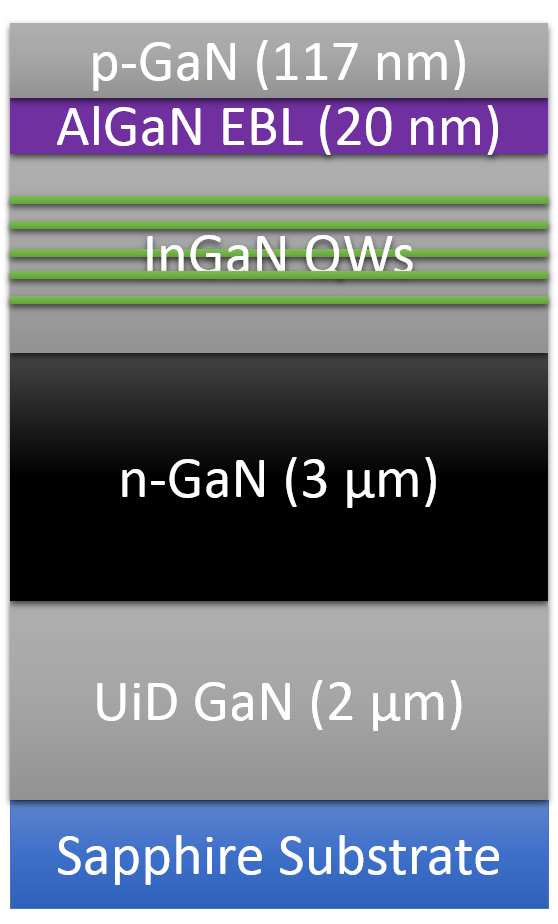
\includegraphics[width=0.4\textwidth]{Figs/Ch3/LEDstruct}
	\caption[h] {LED structure schematic.}
	\label{LEDstruct}
\end{figure}

\FloatBarrier 
The wafer was processed into $1 \times 1 mm^{2}$ side contacted LEDs with thin oxidized Ni/Au current spreading {\it p}-layer Ohmic contact. Ti/Al Ohmic contact stripes were deposited on the {\it n}-layer and the Ni/Au current spreading layer in an interdigitated geometry.\\
QW thickness for the sample was determined from X-ray diffraction \nomenclature[z-XRD]{XRD}{X-ray Diffraction} (XRD) using the method described by Vickers {\it et al.} \cite{Vickers2003}. The QWs were grown using the '2T' method, whereby the growth temperature is ramped up immediately following the InGaN growth under ammonia but without metalorganic fluxes. The barrier growth begins towards the end of the temperature ramp, this typically leads to loss of indium during the temperature ramp which can cause gross well-width fluctuations \cite{Laak2013} but a higher barrier growth temperature is preferable\cite{Oliver2013}. '2T' growth is shown schematically in Fig.\ref{2T}.

\begin{figure}[!ht]
	\centering
	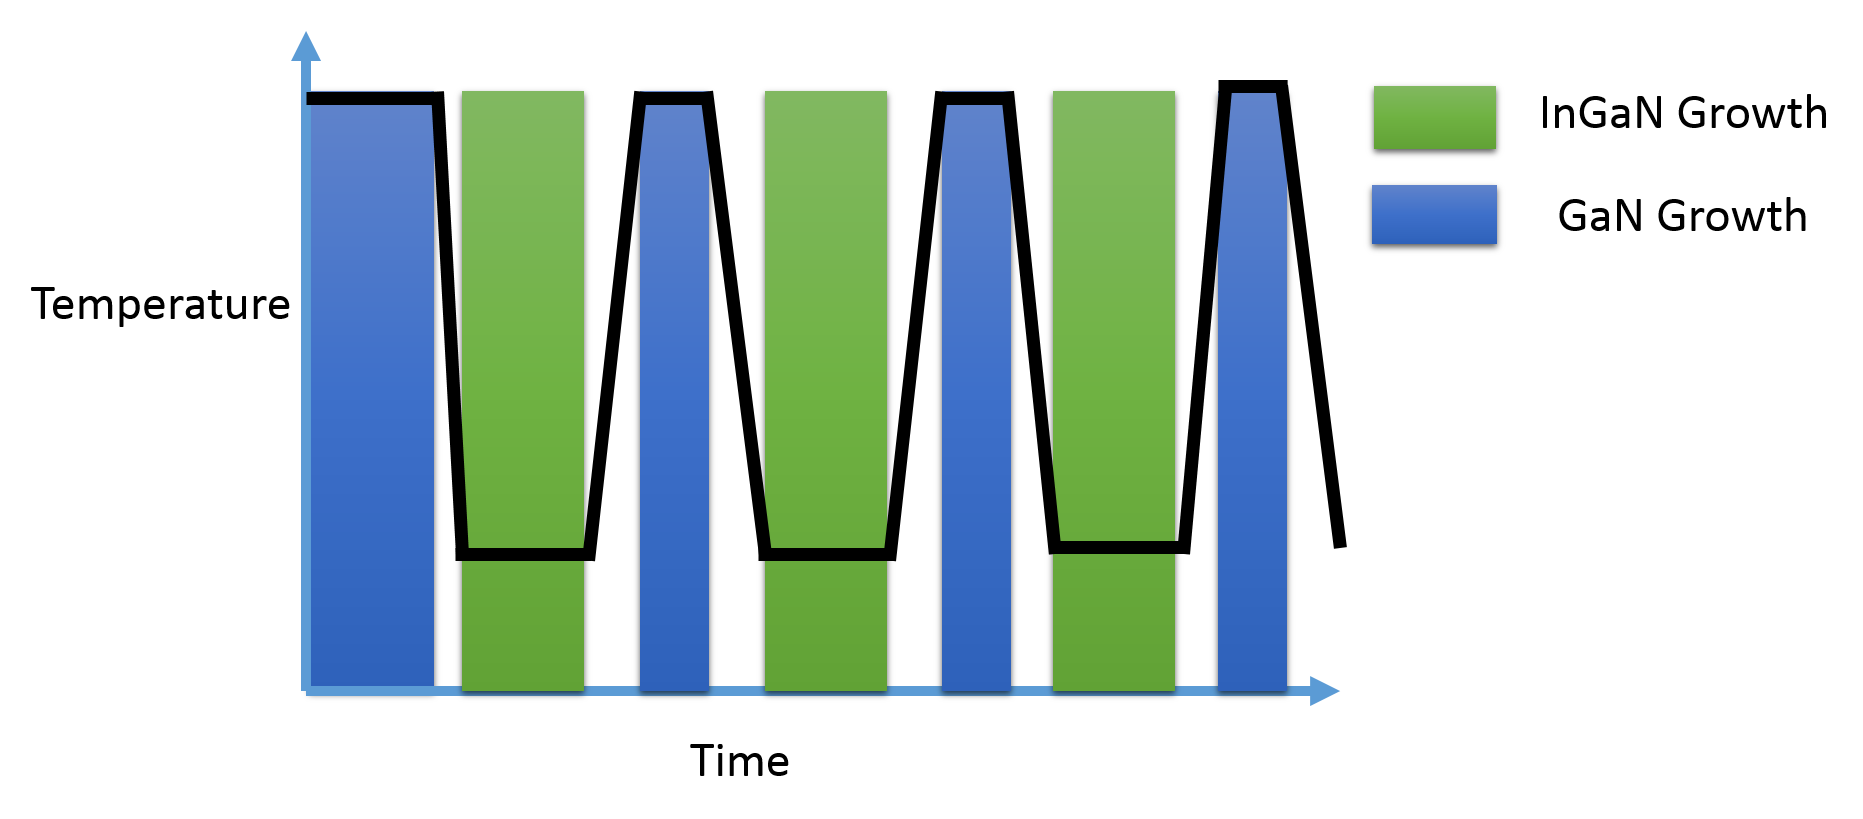
\includegraphics[width=0.9\textwidth]{Figs/Ch3/2T}
	\caption[h] {'2T' growth of InGaN/GaN QWs. GaN QB growth is halted during the temperature ramp. The black trace indicates growth temperature over time.}
	\label{2T}
\end{figure}

\FloatBarrier 

\section{Experimental}

Initial evaluation of the inhomogeneous EL was performed in a Signatone S-1160 probe station under forward bias, as shown in Fig.\ref{probe}.

\begin{figure}[h]
	\centering
	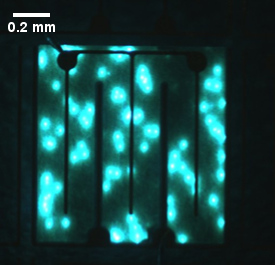
\includegraphics[width=0.4\textwidth]{Figs/Ch3/5608.png}
	\caption {LED EL under a forward bias of 3V. The bright inhomogeneities are visible in the emission of the LEDs. }
	\label{probe}
\end{figure}
\FloatBarrier


Following this, hyperspectral EL mapping with CL and EBIC were performed using a modified Cameca SX100 electron probe micro-analyser with a custom built cathodoluminescence set-up. Hyperspectral EL measurements were performed under forward bias, enabling the acquisition spatially resolved EL maps of the inhomogeneities. Following the detection of hexagonal defects at the centre of inhomogeneities using SEM-CL, the defects were analyzed using AFM and C-AFM. Finally, FIB/SEM lamella preparation techniques were used to perform HAADF-STEM and STEM-EDX on the defects, allowing for access nanoscale compositional and structural information required to reproduce the EL in simulations.


\subsection{Hyperspectral EL Imaging}
Hyperspectral EL imaging was performed at Strathclyde University with the assistance of Dr Michael Wallace. In order to study the device under forward current, the LED wafers were mounted on TO-5 headers and bonded with 5 µm Al wire. A Keithley Instrument 2401 source meter was used to apply varying forward currents to the devices and thus allow for the collection of EL. \\
Full EL spectra were collected with a spatial resolution of approximately 3 µm and analysed using custom software developed by Dr. Paul Edwards, allowing for 2-D maps of EL peak intensity, position and FWHM. At each pixel in the map, a full EL spectrum was collected by an Andor CCD camera. A full set of data extracted from the hyperspectral EL mapping is shown in Fig.\ref{ELfull}

\begin{figure}[!ht]
	\centering
	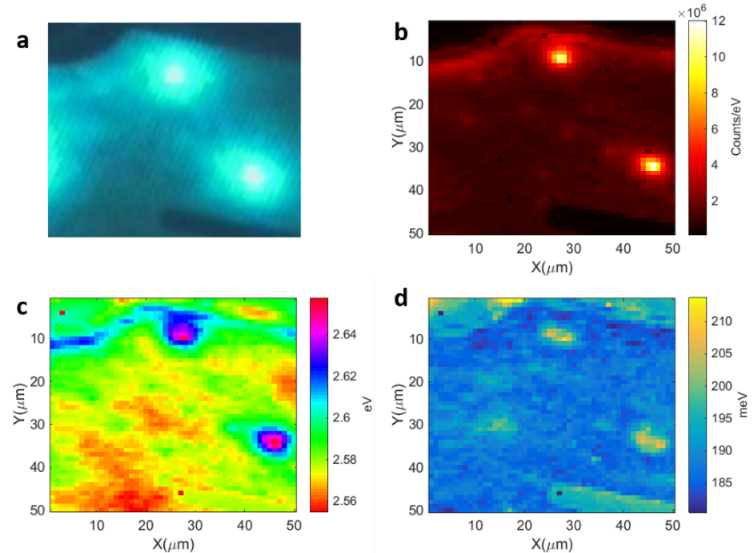
\includegraphics[width=0.8\textwidth]{Figs/Ch3/ELfull}
	\caption[h] {a) Probe station image b) EL peak intensity, c) EL peak energy and d) EL FWHM extracted by fitting the hyperspectral EL data under a forward current of 10 mA}
	\label{ELfull}
\end{figure}

\FloatBarrier 

It is interesting to note that from this representative data set, the inhomogeneities observed are brighter by a factor of $\sim 6$, blue-shifted in terms of peak energy by $\sim 0.08$ eV and have a larger FWHM. Although these values were observed to shift based on injection current, the overall trend observed in the EL data collected for this LED is represented by Fig.\ref{ELfull}.

\subsubsection{Current Dependent EL Measurements}

Current dependent hyperspectral EL maps of the same area were performed, in order to examine the behaviour of the inhomogeneities with increasing current relative to the 'uniform' background. The peak intensities and peak energies for injection currents for device C5608A ranging from 1-250 mA are shown in Figures \ref{peak5610} and \ref{centre5610} respectively. 

\begin{figure}
	\begin{subfigure}[b]{0.48\textwidth}
		\centering
		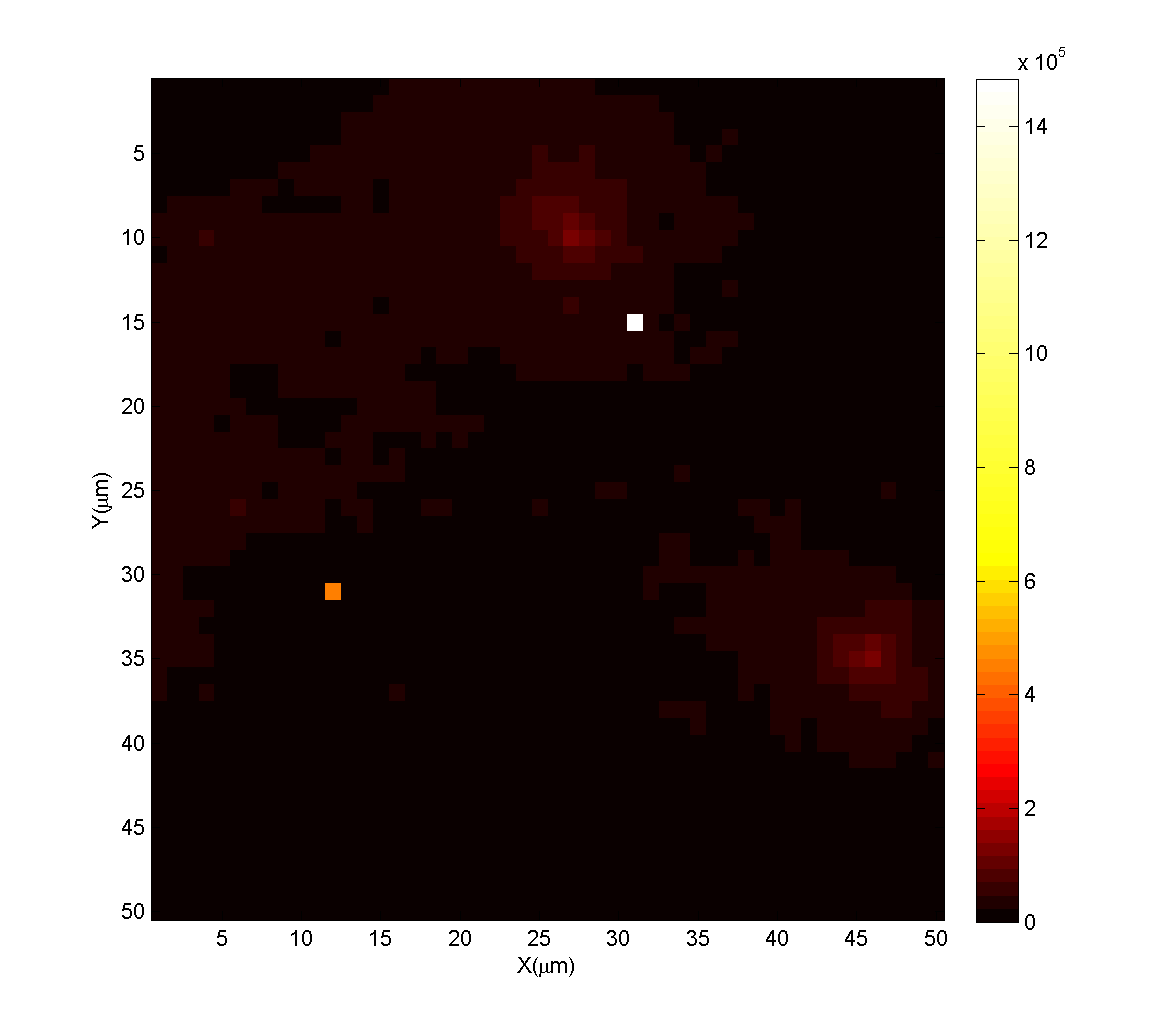
\includegraphics[width=1\linewidth]{Figs/Ch3/1c}
		\caption{1 mA}
	\end{subfigure}%
	\hspace*\fill
	\begin{subfigure}[b]{0.48\textwidth}
		\centering
		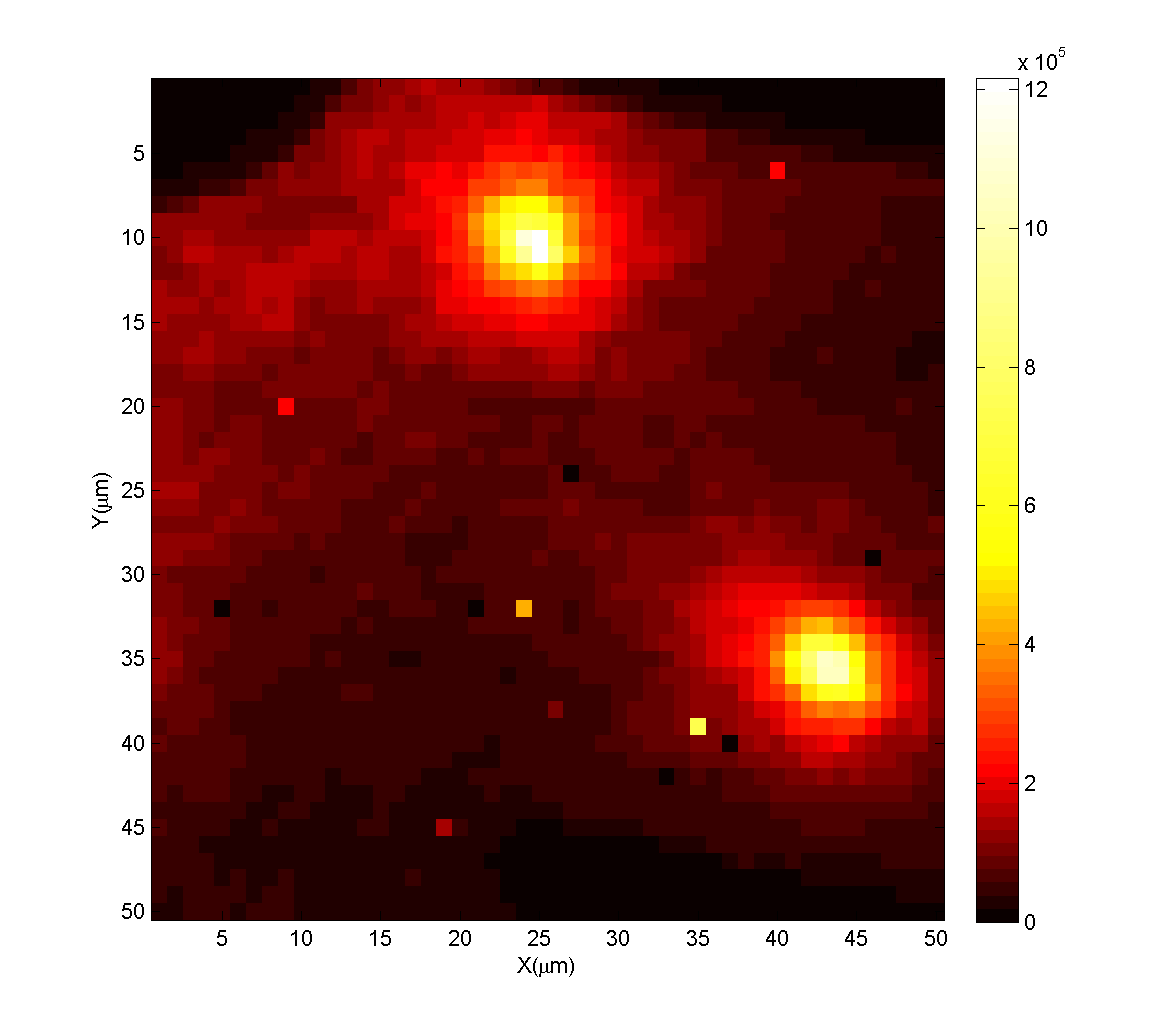
\includegraphics[width=1\linewidth]{Figs/Ch3/2dot5c}
		\caption{5 mA}		
	\end{subfigure}%
	
	\medskip
	\begin{subfigure}[b]{0.48\textwidth}
		\centering
		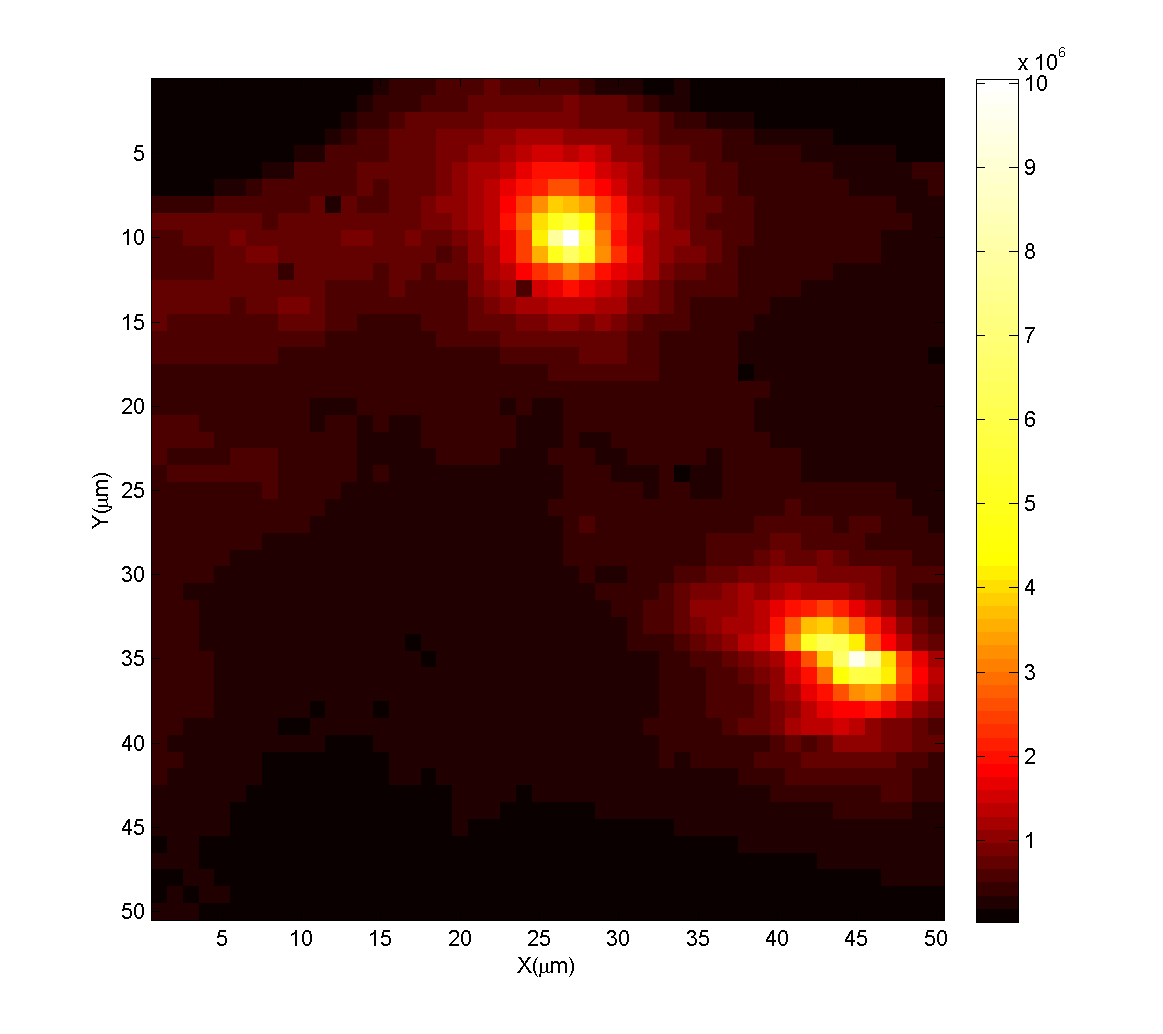
\includegraphics[width=1\linewidth]{Figs/Ch3/10c}
		\caption{10 mA}
	\end{subfigure}%
	\hspace*\fill
	\begin{subfigure}[b]{0.48\textwidth}
		\centering
		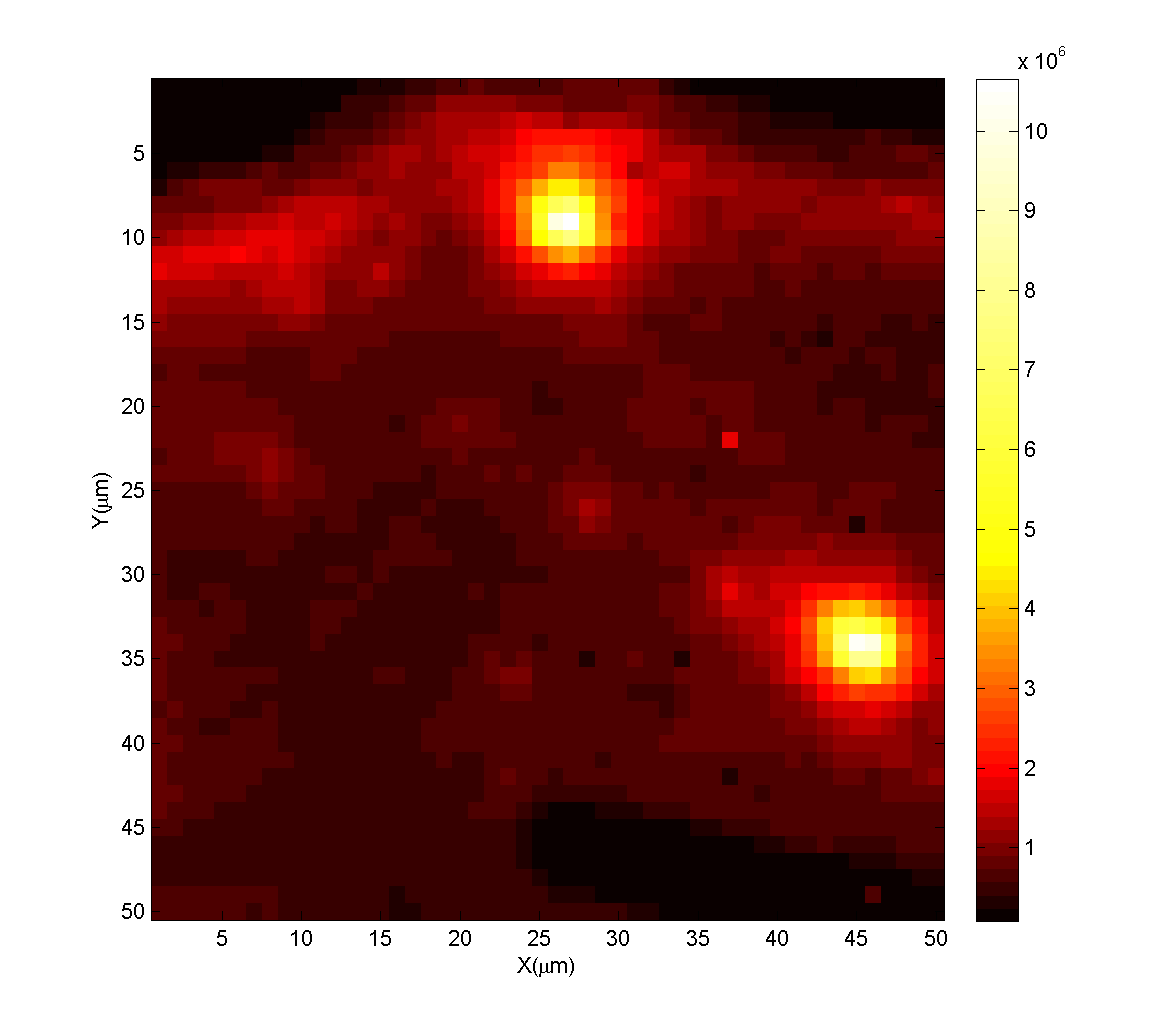
\includegraphics[width=1\linewidth]{Figs/Ch3/50c}
		\caption{50 mA}		
	\end{subfigure}%
	
	\medskip
	\begin{subfigure}[b]{0.48\textwidth}
		\centering
		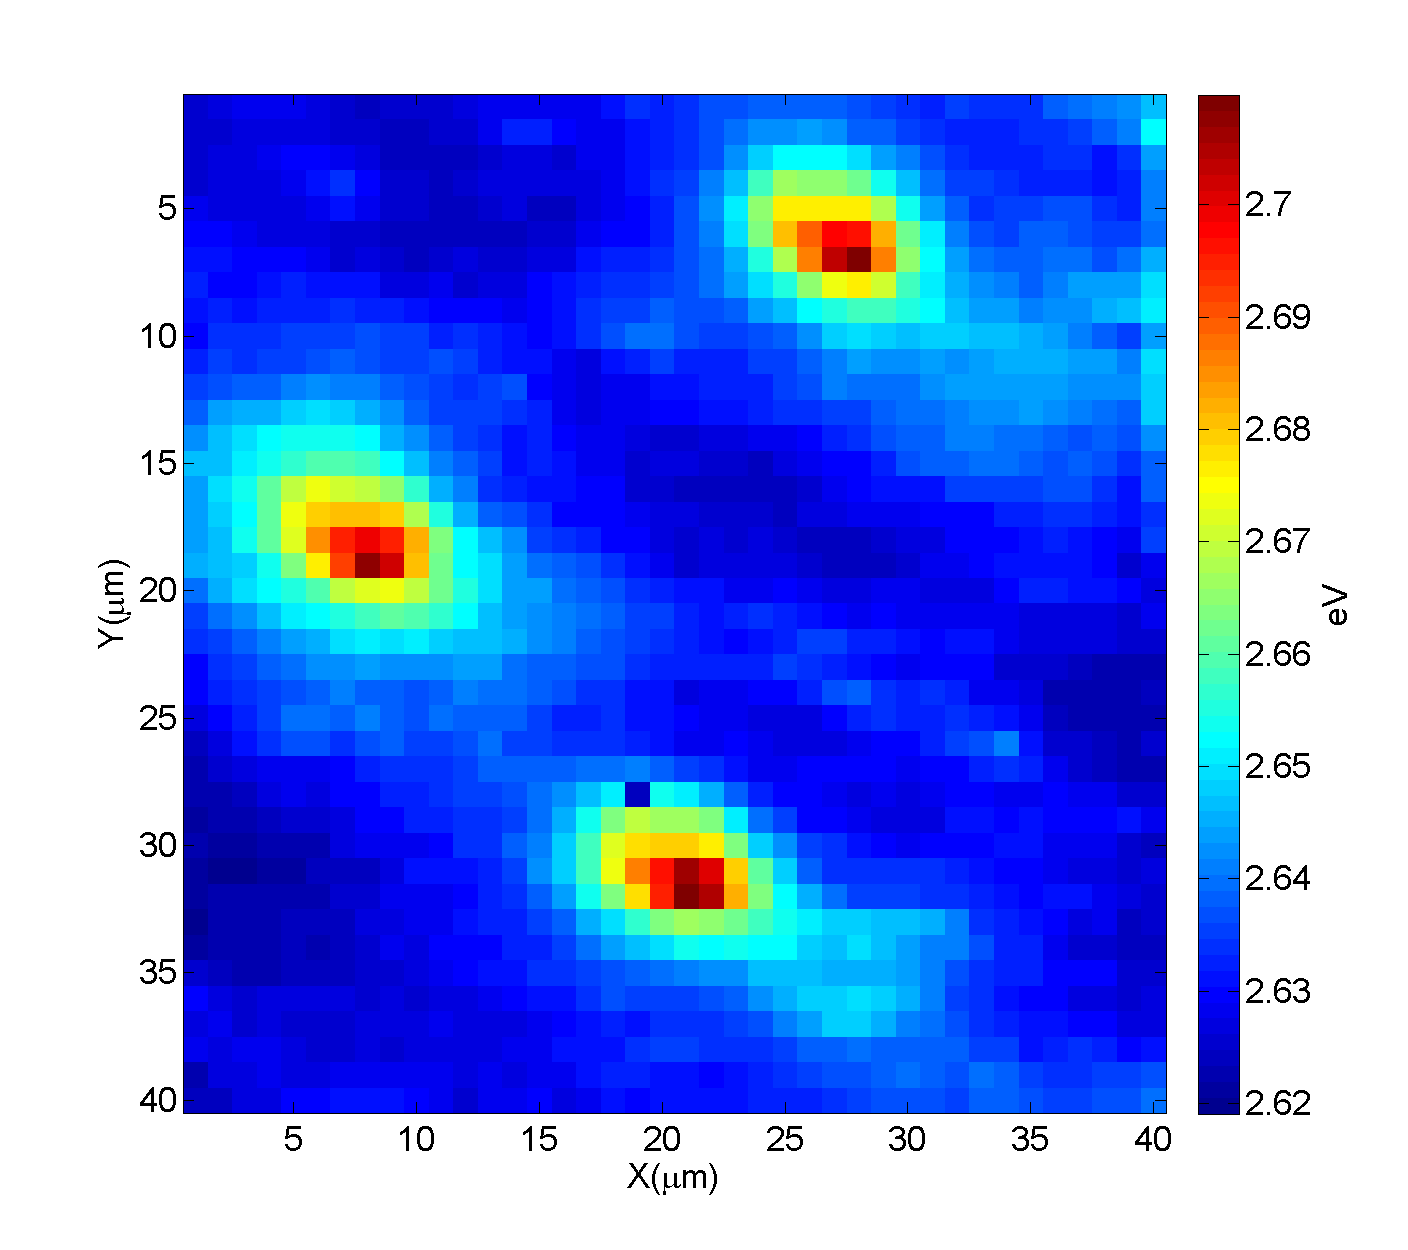
\includegraphics[width=1\linewidth]{Figs/Ch3/100c}
		\caption{100 mA}
	\end{subfigure}%
	\hspace*\fill
	\begin{subfigure}[b]{0.48\textwidth}
		\centering
		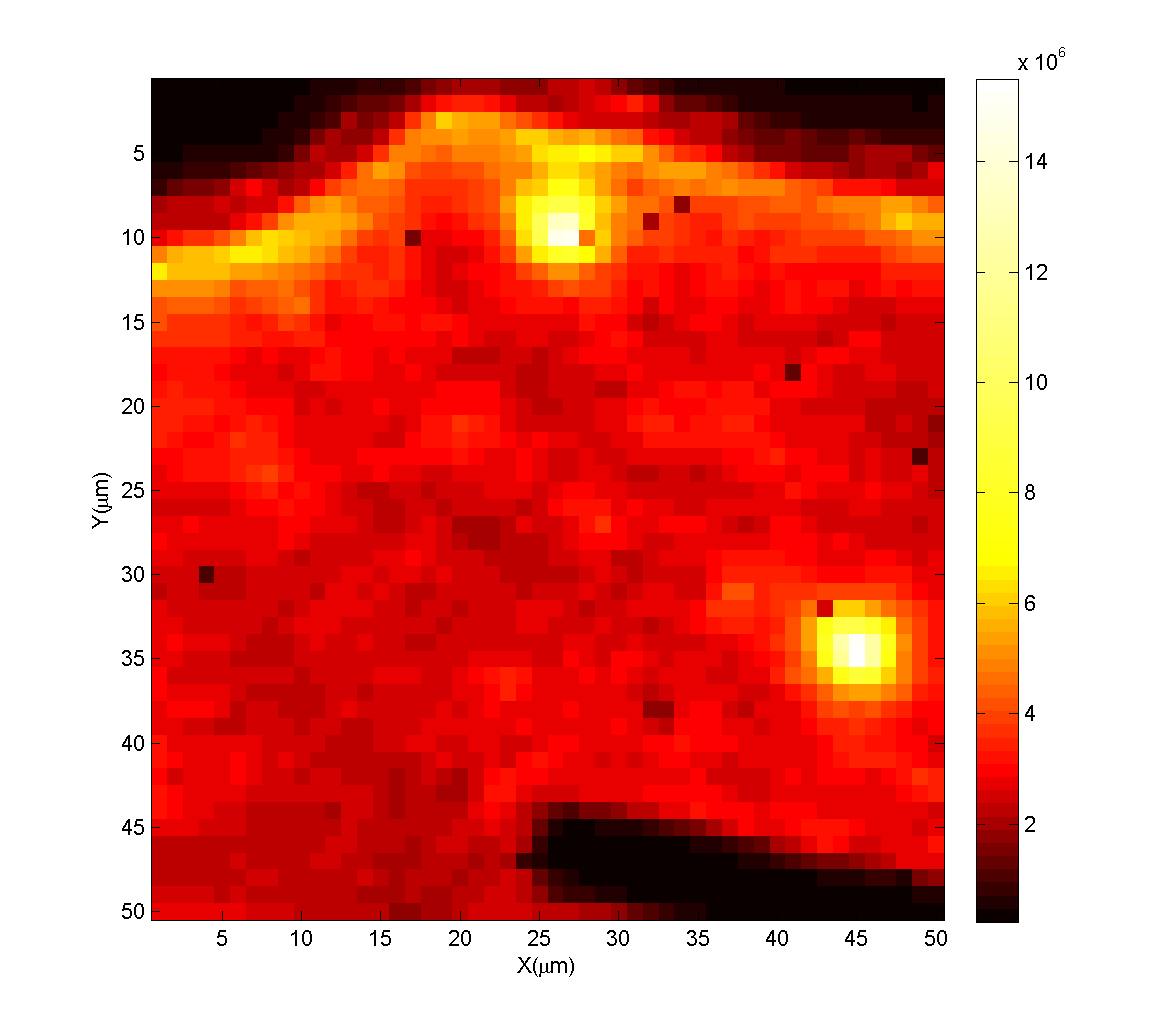
\includegraphics[width=1\linewidth]{Figs/Ch3/250c}
		\caption{250 mA}		
	\end{subfigure}%
	
	\caption{Peak intensity for varying injection current for C5608.}
	\label{peak5610}
\end{figure}

\begin{figure}
	\begin{subfigure}[b]{0.48\textwidth}
		\centering
		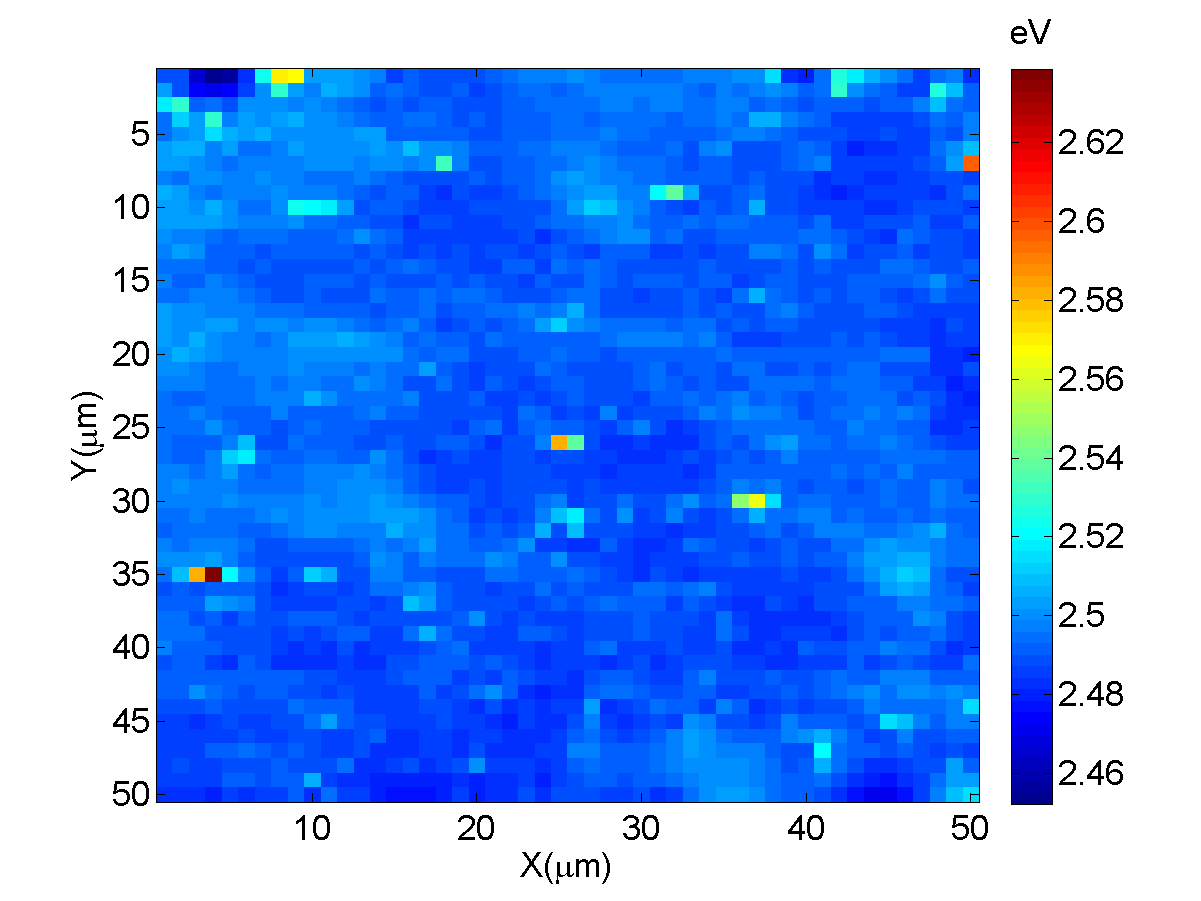
\includegraphics[width=1\linewidth]{Figs/Ch3/1}
		\caption{1 mA}
	\end{subfigure}%
	\hspace*\fill
	\begin{subfigure}[b]{0.48\textwidth}
		\centering
		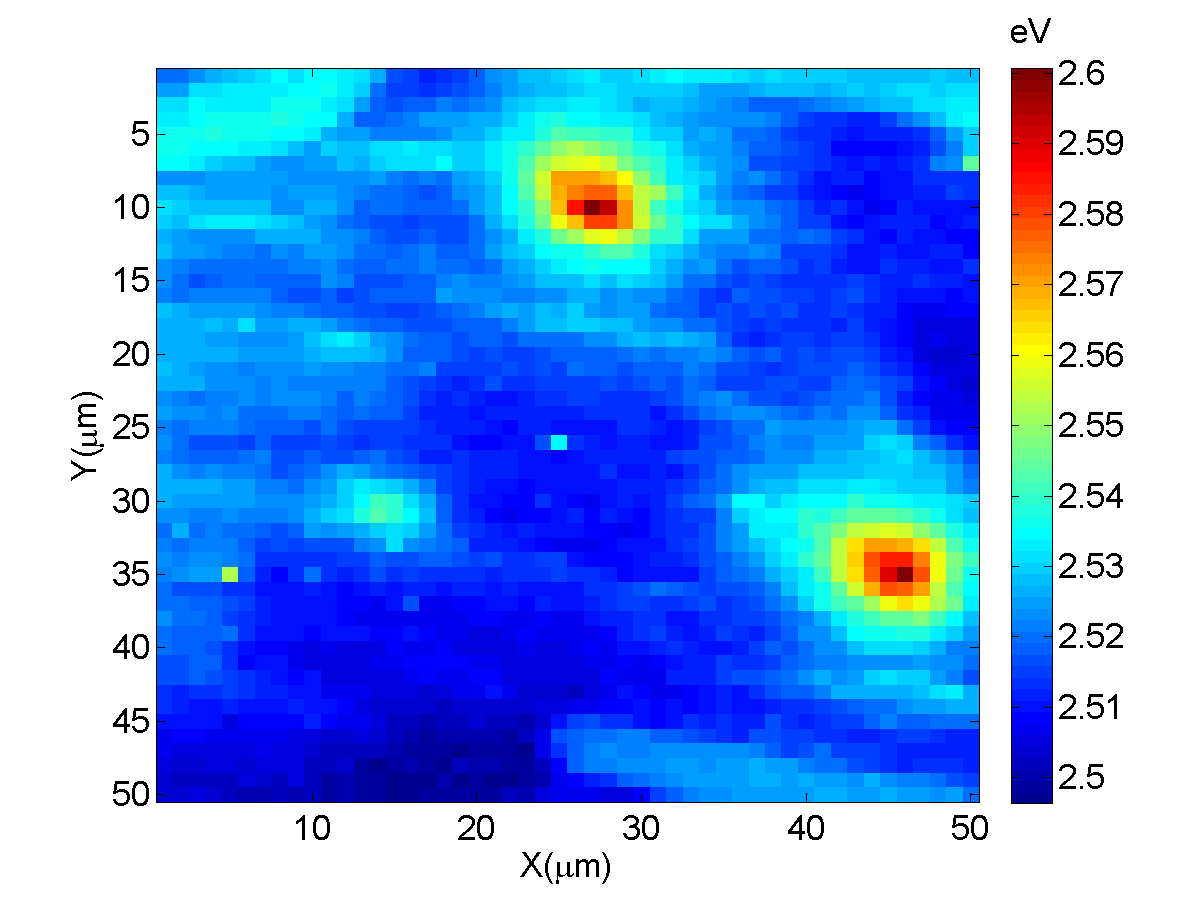
\includegraphics[width=1\linewidth]{Figs/Ch3/5}
		\caption{5 mA}		
	\end{subfigure}%
	
	\medskip
	\begin{subfigure}[b]{0.48\textwidth}
		\centering
		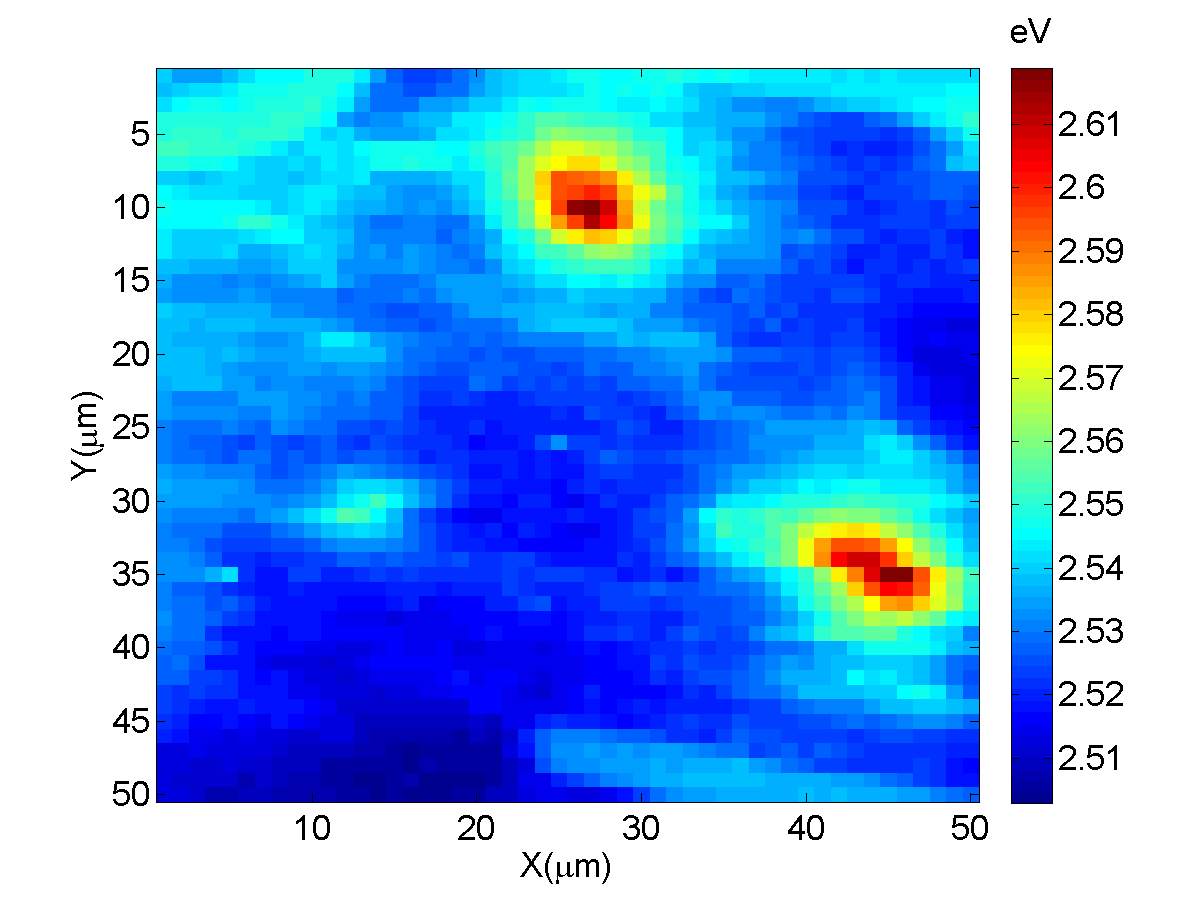
\includegraphics[width=1\linewidth]{Figs/Ch3/10}
		\caption{10 mA}
	\end{subfigure}%
	\hspace*\fill
	\begin{subfigure}[b]{0.48\textwidth}
		\centering
		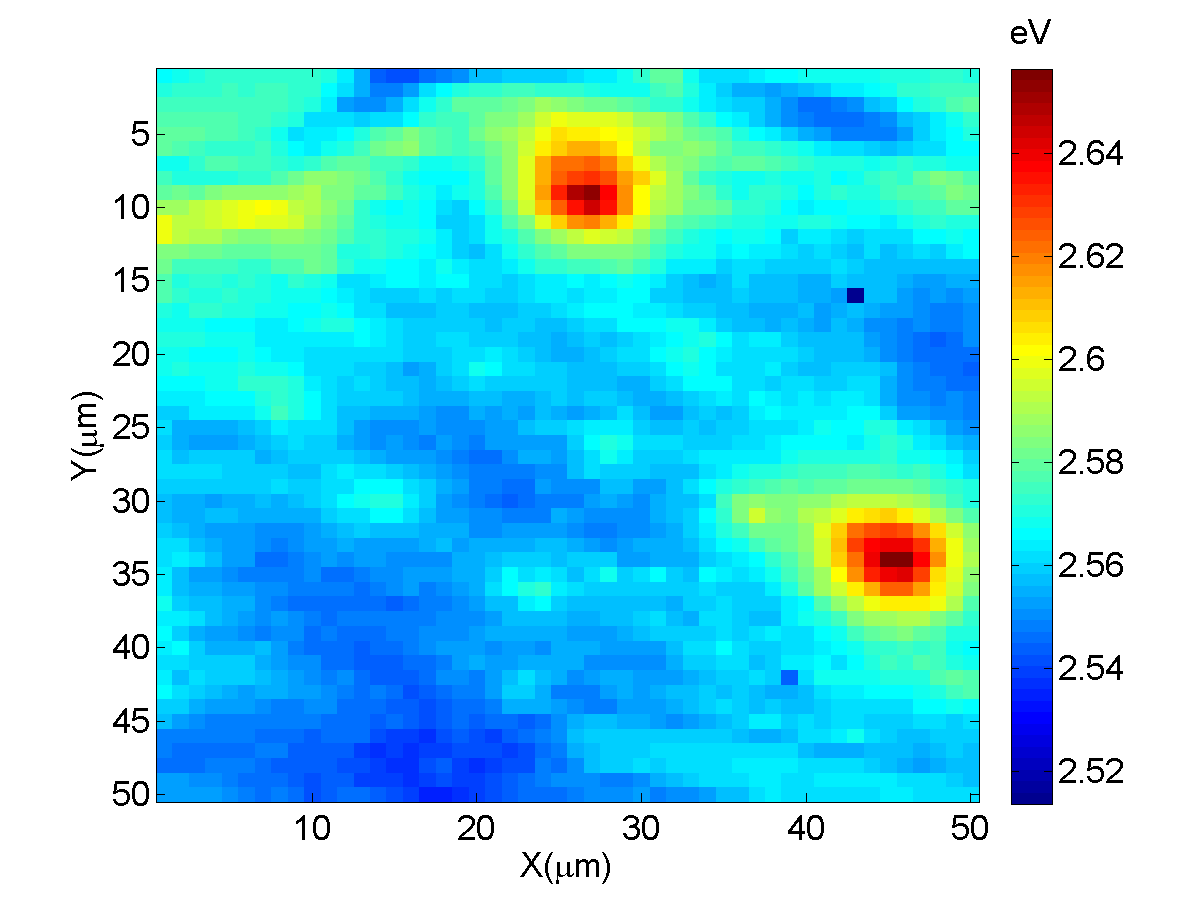
\includegraphics[width=1\linewidth]{Figs/Ch3/50}
		\caption{50 mA}		
	\end{subfigure}%
	
	\medskip
	\begin{subfigure}[b]{0.48\textwidth}
		\centering
		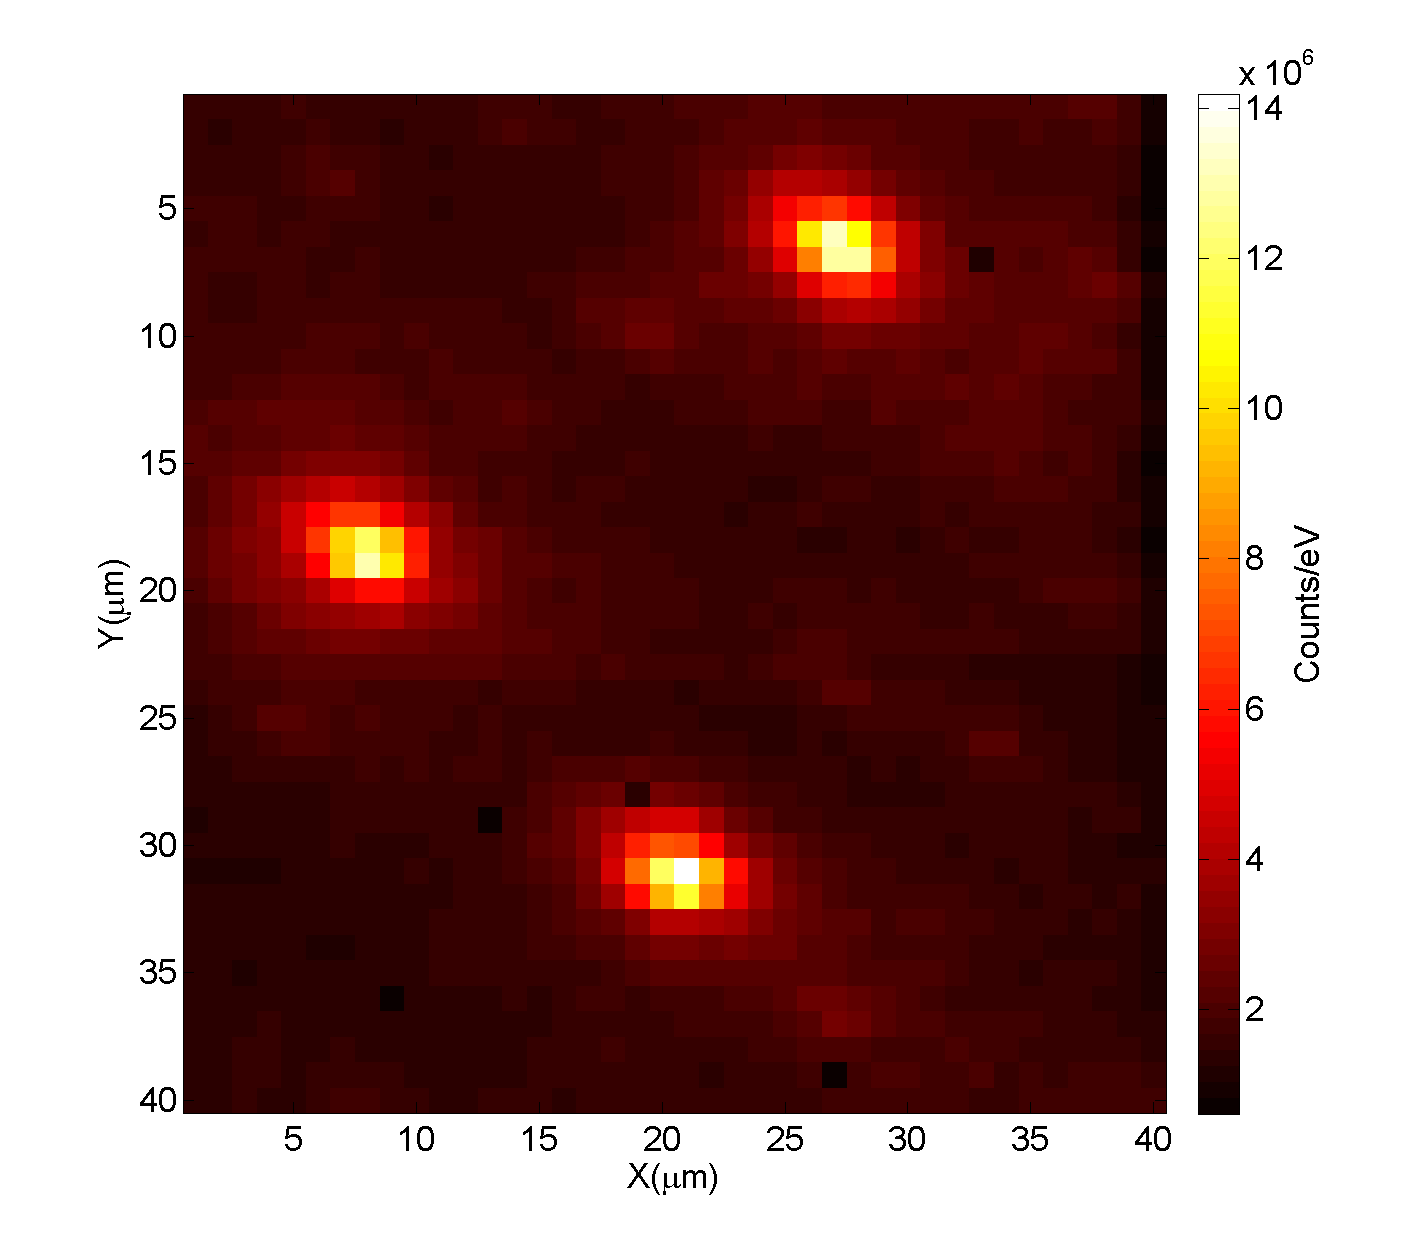
\includegraphics[width=1\linewidth]{Figs/Ch3/100}
		\caption{100 mA}
	\end{subfigure}%
	\hspace*\fill
	\begin{subfigure}[b]{0.48\textwidth}
		\centering
		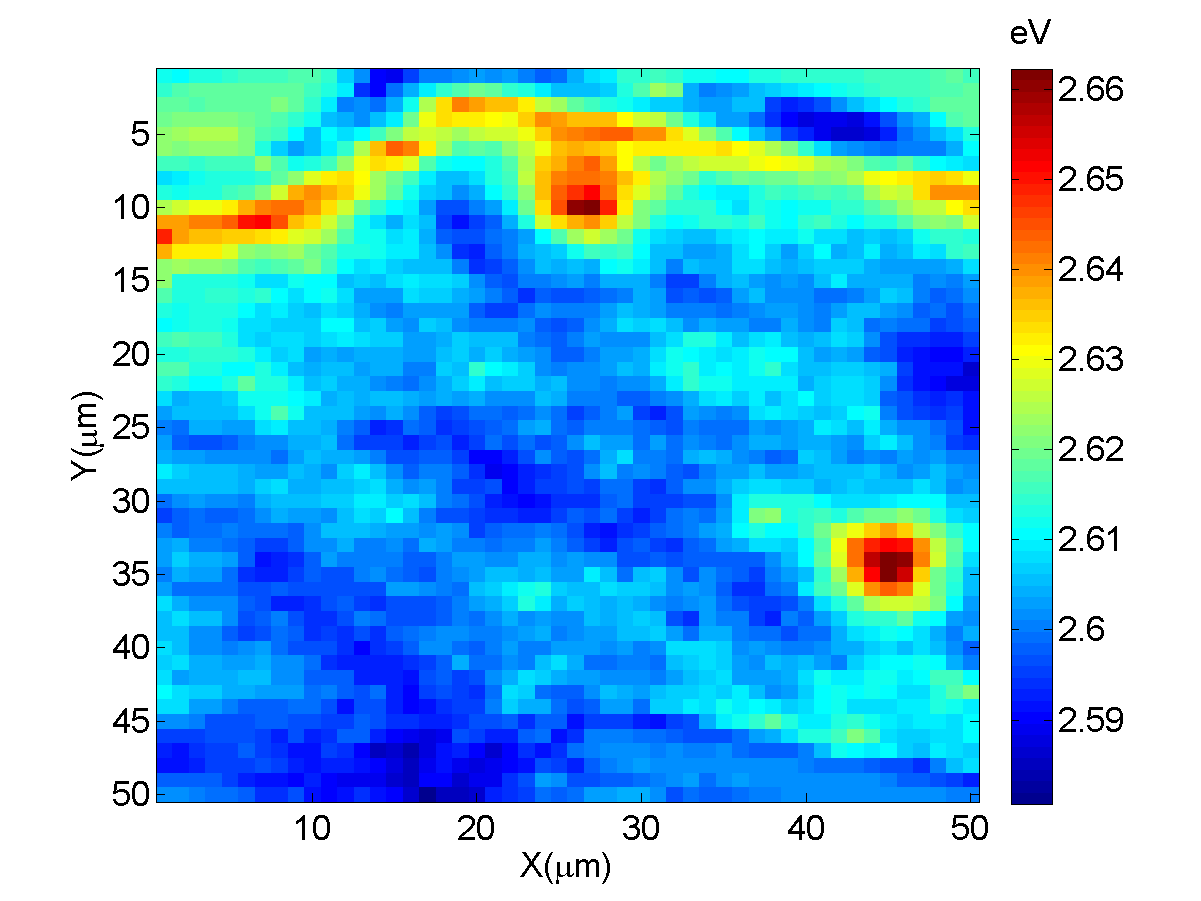
\includegraphics[width=1\linewidth]{Figs/Ch3/250}
		\caption{250 mA}		
	\end{subfigure}%
	
	\caption{Peak energy for varying injection current for C5608.}
	\label{centre5610}
\end{figure}

\FloatBarrier

The spatially resolved EL data shown in Figures \ref{peak5610} and \ref{centre5610} allow for the comparison between areas containing the inhomogeneities and the 'background' EL. This is demonstrated in Fig. \ref{5610peakcomp} which shows the behaviour of both the inhomogeneities (labelled 'spots') and the averaged background peak intensity with increasing injection current.
\begin{figure}[!ht]
	\centering
	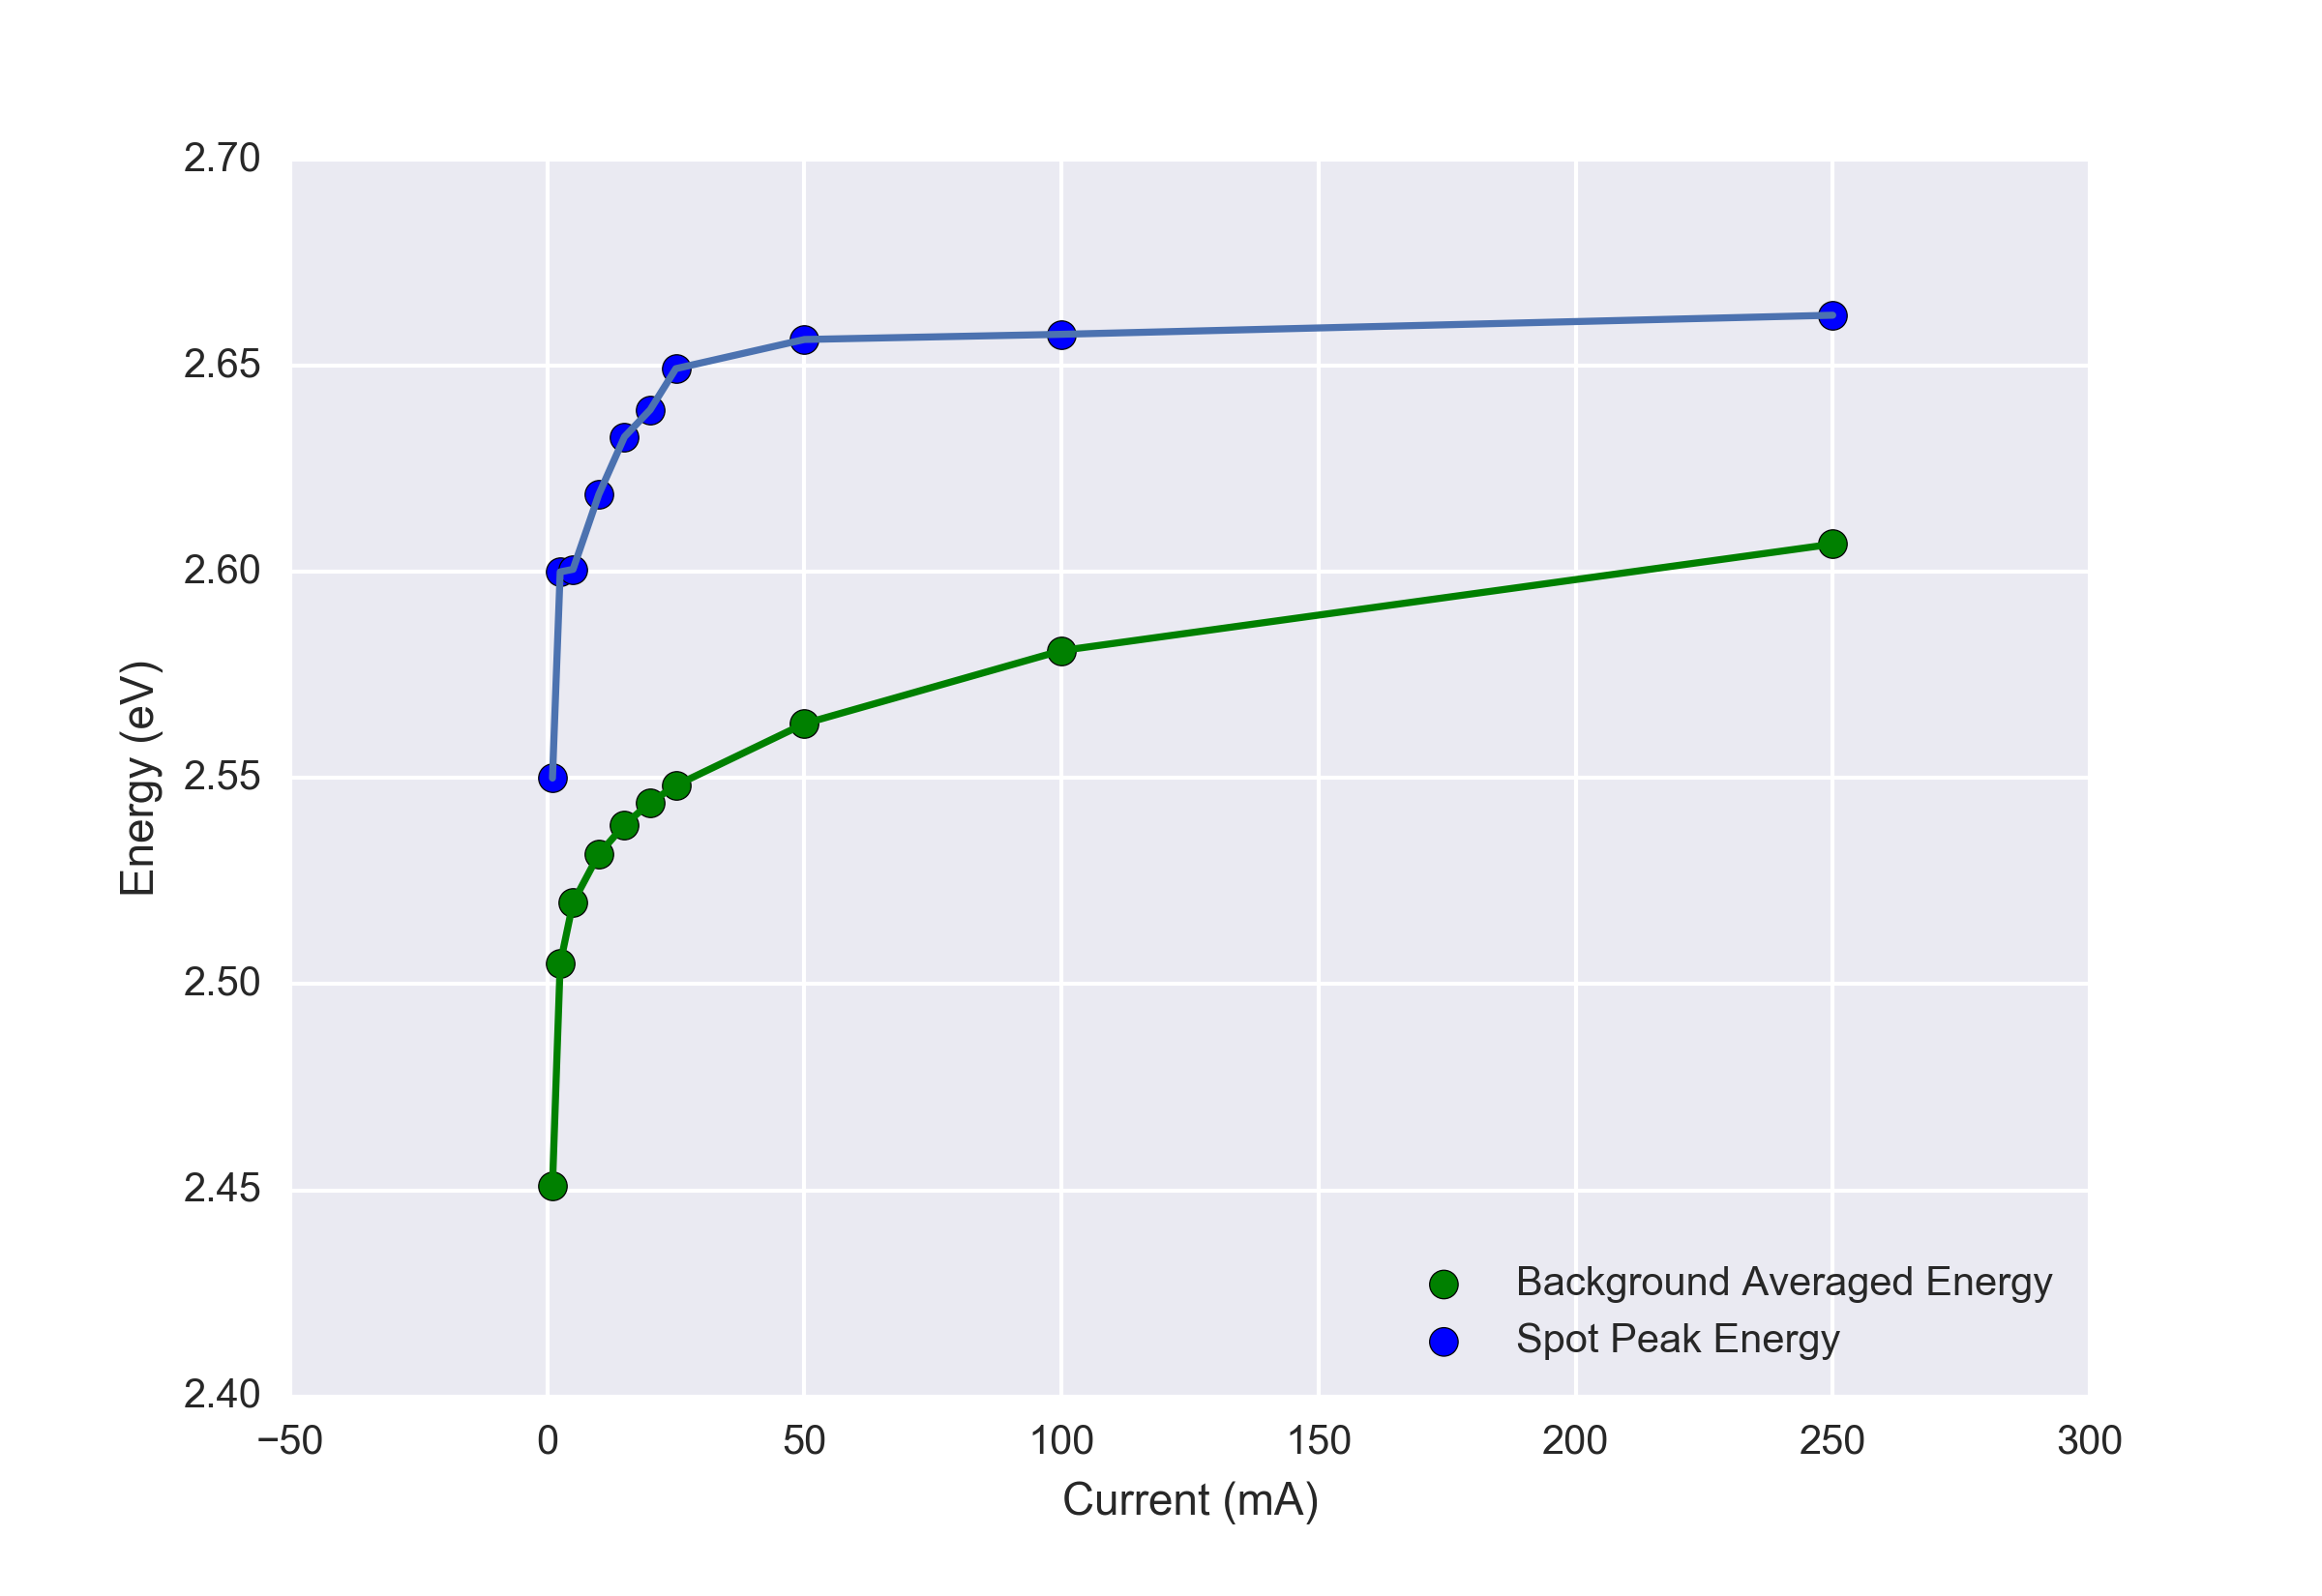
\includegraphics[width=0.8\textwidth]{Figs/Ch3/centrePeakcomp5608.png}
	\caption[h] {Spot and background average peak intensity against injection current}
	\label{5610peakcomp}
\end{figure}

\FloatBarrier 
It is interesting to note that Fig.\ref{5610peakcomp} shows the inhomogeneities experience a far sharper initial increase in peak intensity relative to the background based on the hyperspectral EL data fitting in the current range 0-50 mA, perhaps indicating enhanced current injection in the areas exhibiting the inhomogeneities.\\
Fig. \ref{5610centrecomp} shows the same current dependent comparison for background and inhomogeneity peak energy. Here we see the same trend, in that the inhomogeneity exhibits a larger current-induced blueshift in the 0-50 mA range relative to the background. The origin of the current-dependent blueshift in InGaN QW structures is attributed to the screening of the QCSE by the additional carriers injected into the wells \cite{Ryou2009}, and as such indicates the inhomogeneities are regions experiencing higher current injection relative to the background.

\begin{figure}[!ht]
	\centering
	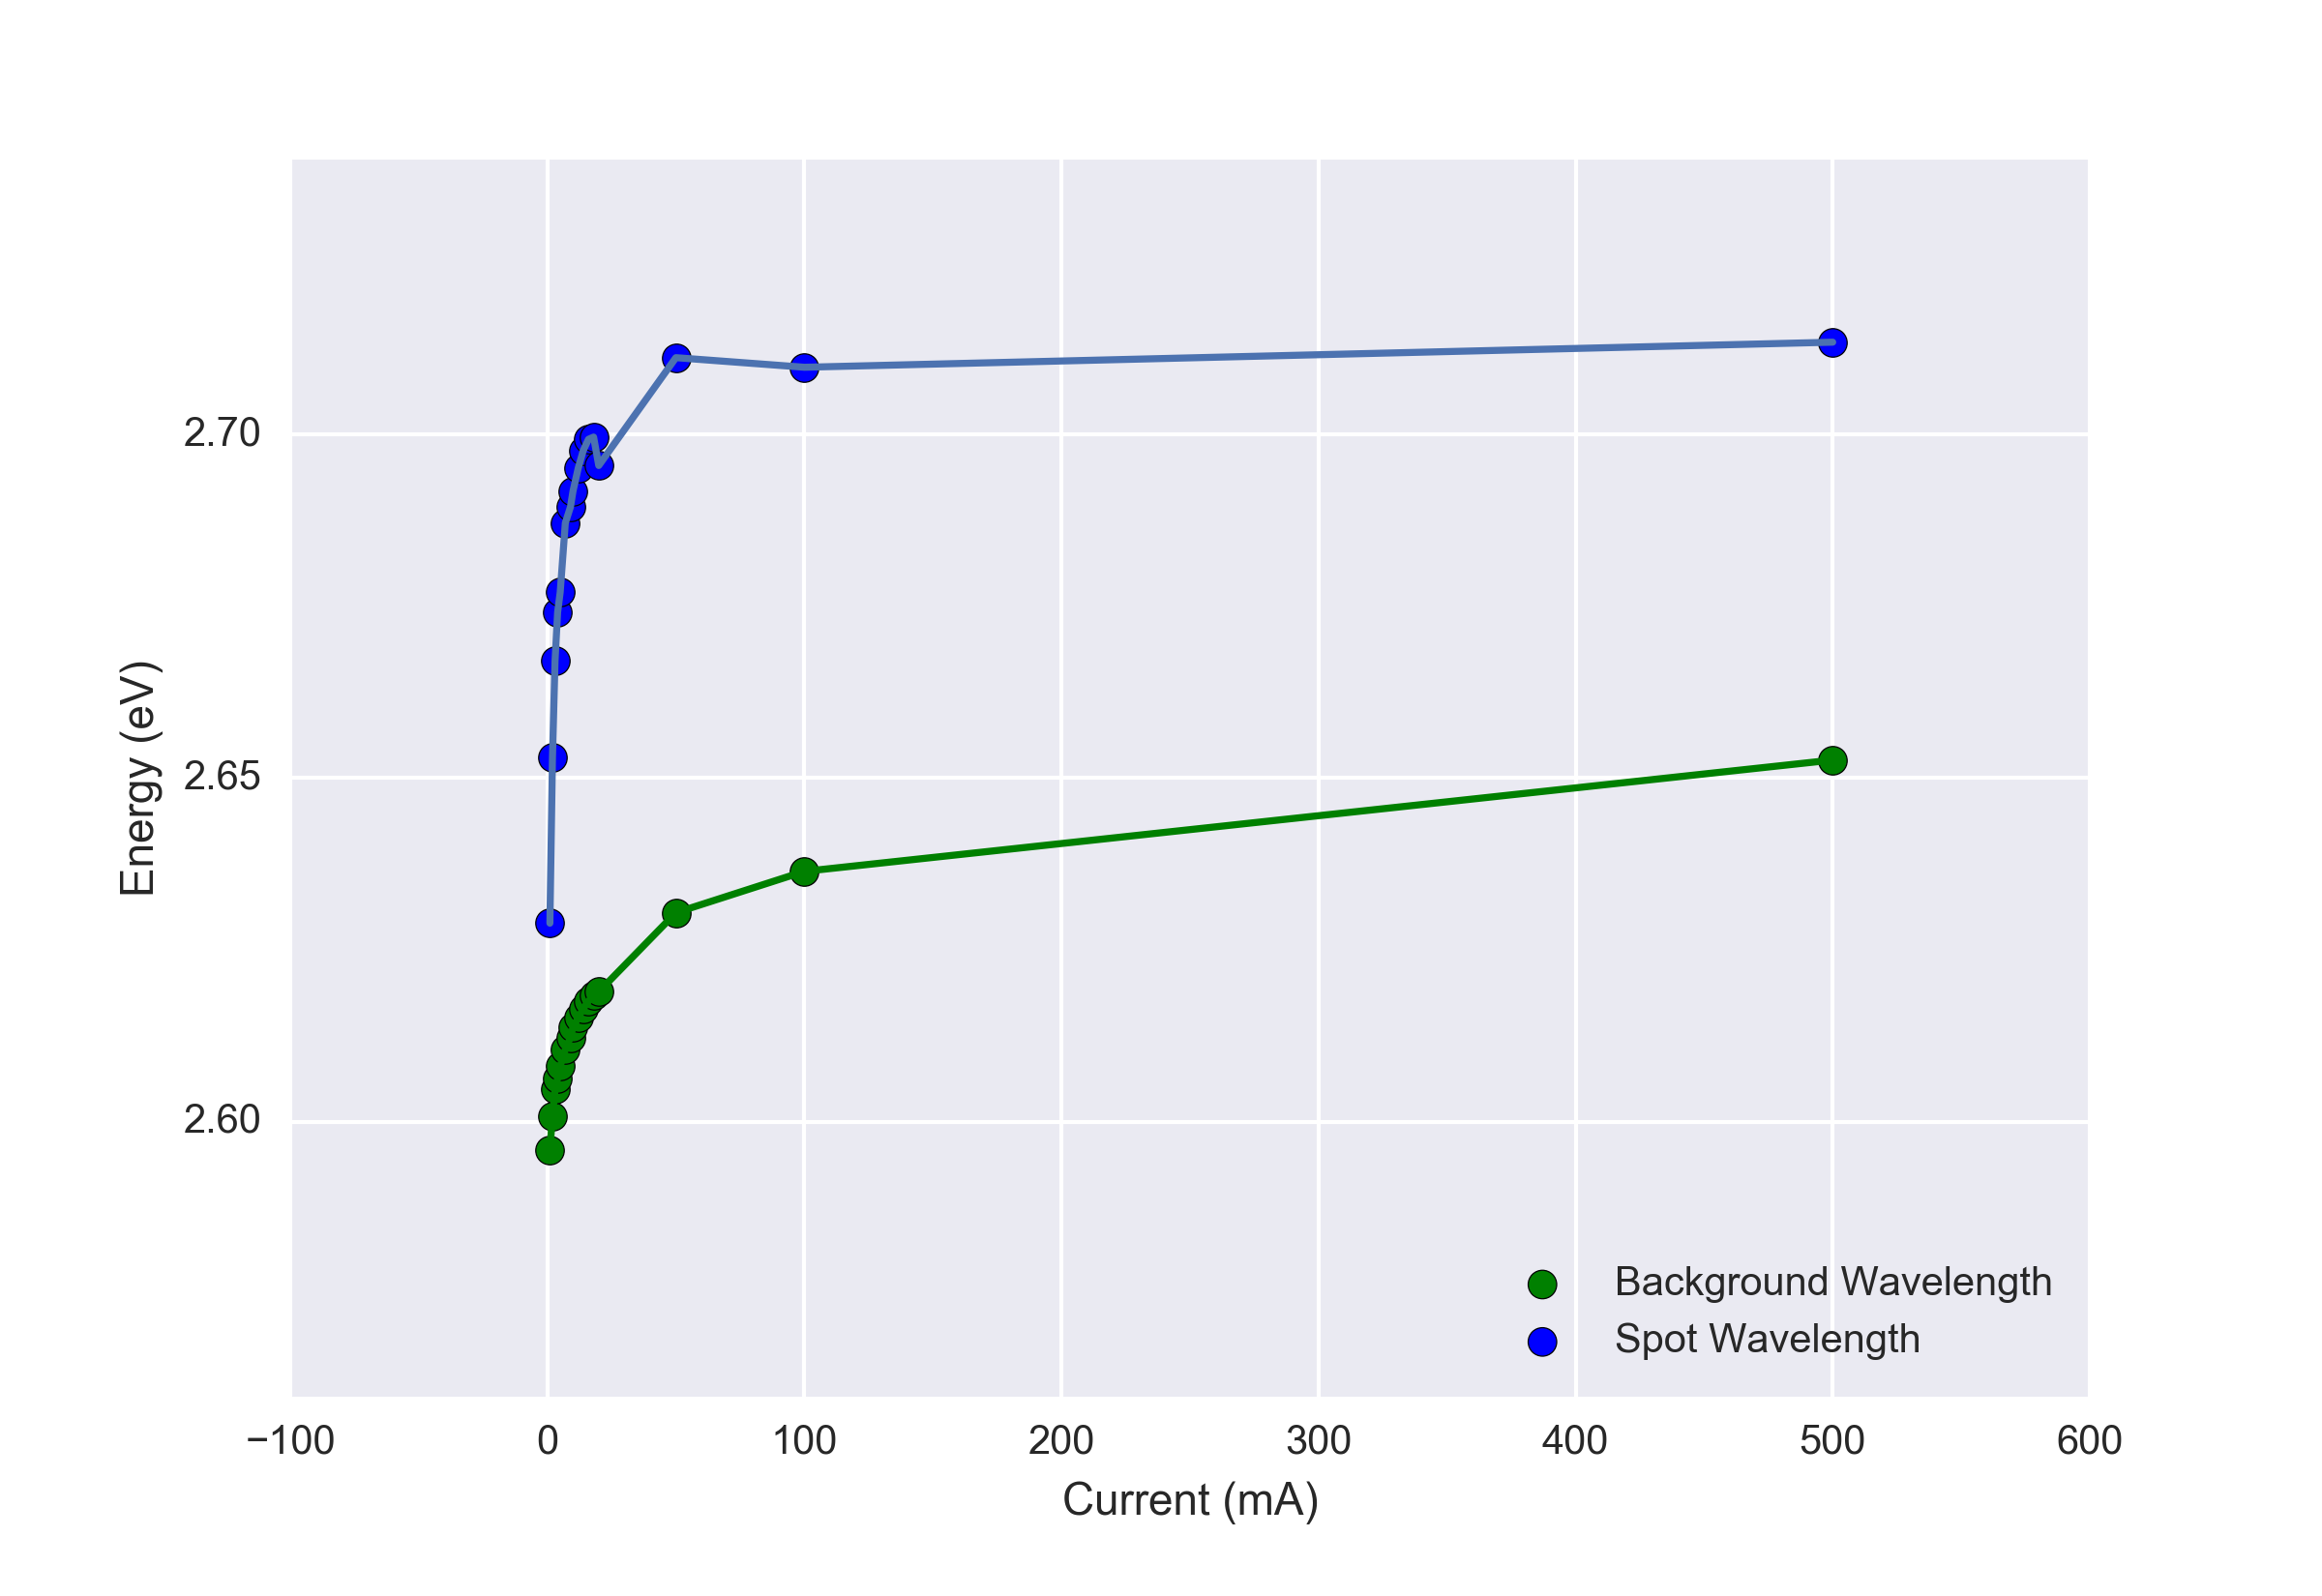
\includegraphics[width=0.8\textwidth]{Figs/Ch3/CentercompeV.png}
	\caption[h] {Spot and background average peak energy against injection current}
	\label{5610centrecomp}
\end{figure}

\FloatBarrier 


\subsection{Cathodoluminescence and Electron Beam Induced Current}
Having noted the behaviour of the inhomogeneities inferred from the hyperpsectral EL data, CL and EBIC data were taken over areas containing the inhomogeneities in order to examine their properties in more detail as electron-beam based techniques allow for a far higher resolution than EL mapping.\\
In order to achieve simultaneous CL and EBIC measurements, a Keithley Instrument 2401 source/measure unit was utilised in order to main the LED devices at a fixed bias of 0V thus allowing for the measurement of the short circuit current. During the CL image scanning, the Andor CCD camera was set-up to trigger the unit to record the current at each point in the CL spectral acquisition. The CL acquisition was performed with an electron beam at 10 kV and 1 nA. Unfortunately the secondary electron detector was inoperable during the acquisition of this data, as such there is no accompanying SEM micrograph for the CL and EBIC data. The CL and EBIC data for C5608A are shown in Fig.\ref{5608CLEBIC}.

\begin{figure}[h]
	\hspace*{0.5cm}
	\begin{subfigure}[b]{0.48\textwidth}
		\centering
		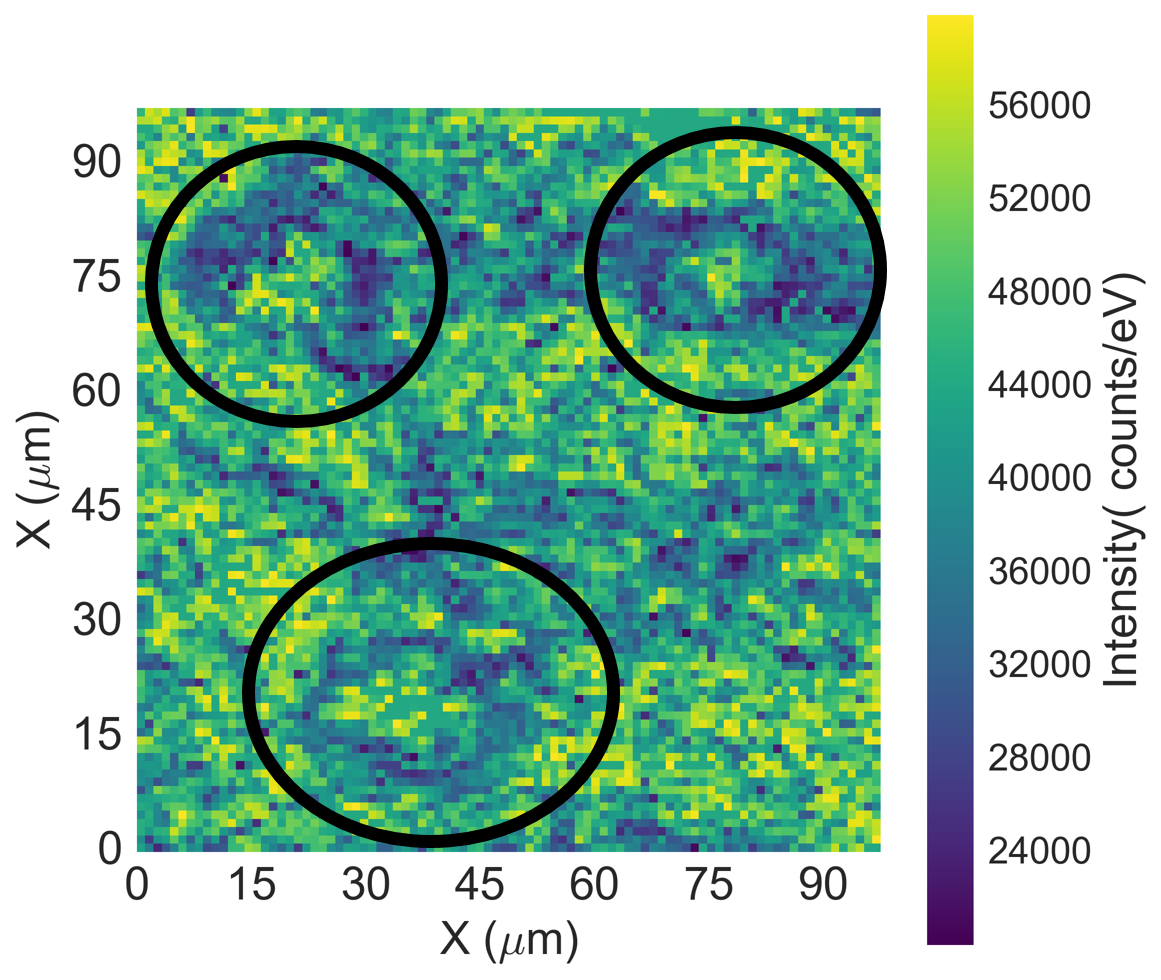
\includegraphics[width=1\linewidth]{Figs/Ch3/5608AsmallCL}
		\caption{}
		
	\end{subfigure}%
	\hspace*{0.5cm}
	\begin{subfigure}[b]{0.48\textwidth}
		\centering
		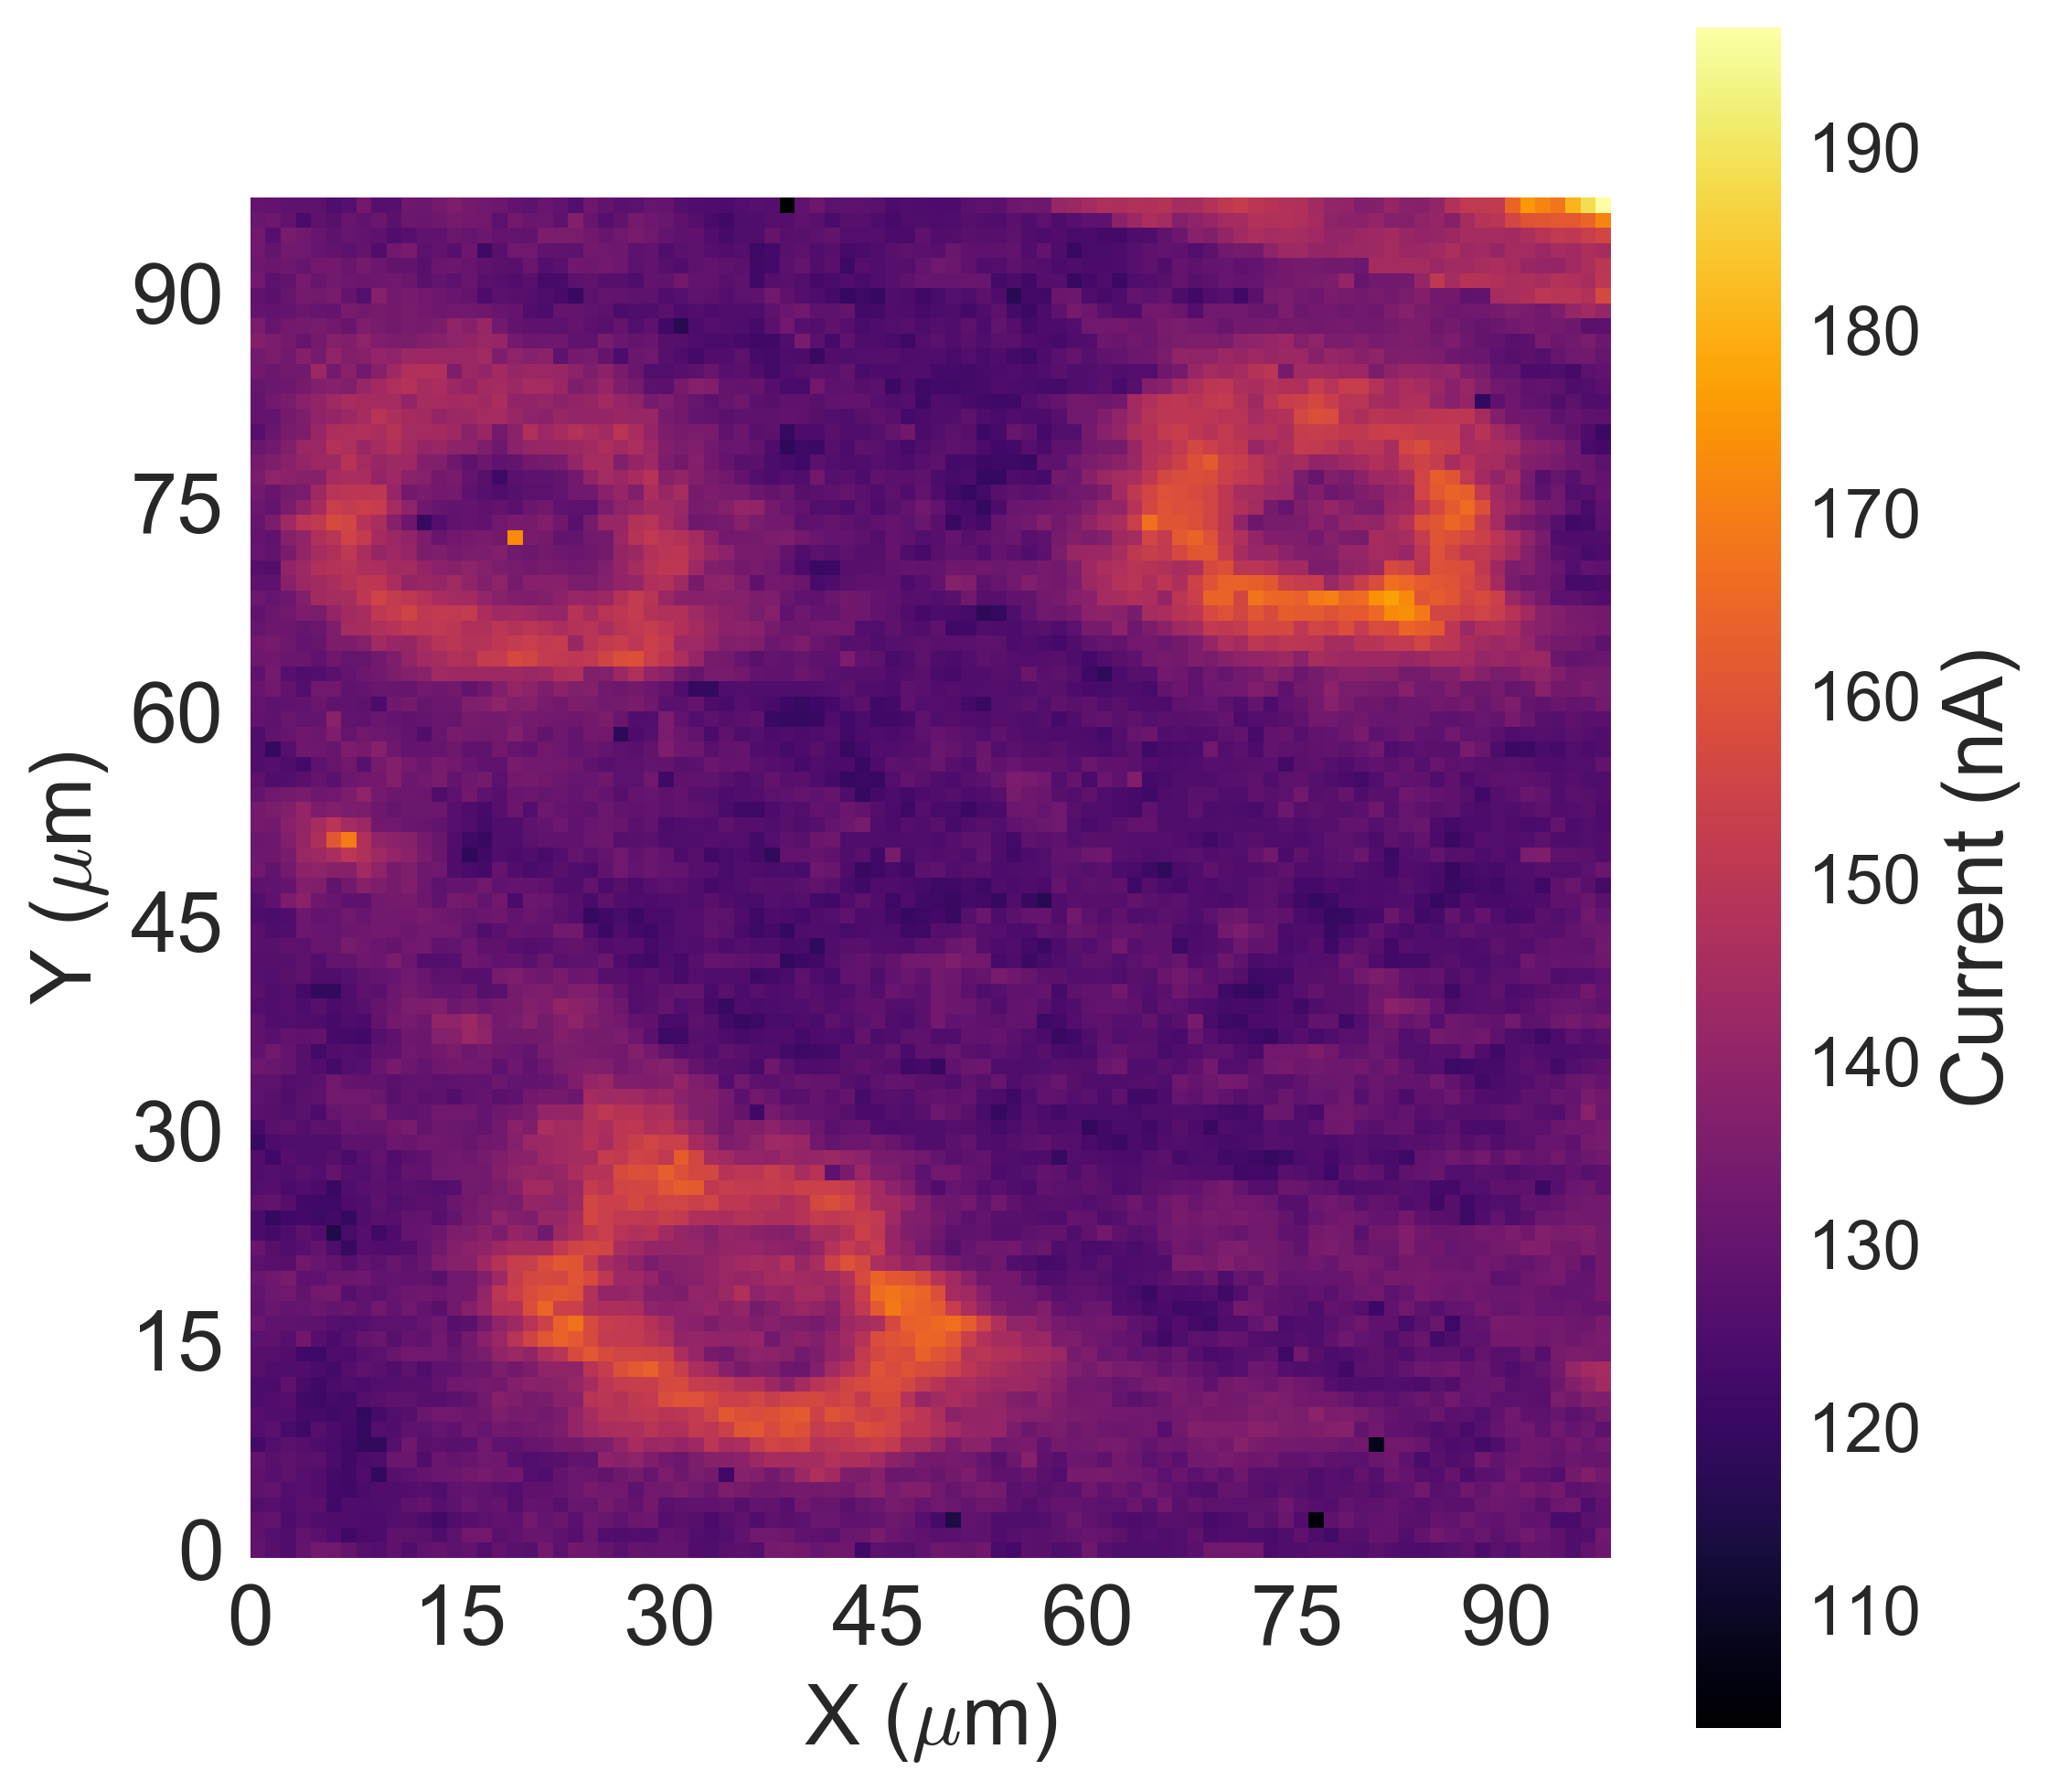
\includegraphics[width=0.98\linewidth]{Figs/Ch3/5608smallEBIC}
		\caption{}
	\end{subfigure}%
	
	\caption{a) CL and b) EBIC maps acquired simultaneously of the area shown in Fig.\ref{5610loc}b.}
	\label{5608CLEBIC}
\end{figure}
\FloatBarrier

Fig. \ref{5608CLEBIC}a. shows the inhomogeneities exhibit a lower CL intensity relative to the background, in contrast to the EL. Interestingly, the EBIC signal, shown in Fig.\ref{5608CLEBIC} for both inhomogeneities examined seem rather different. The feature closest to the contact region can be seen as a region of high EBIC surrounding a region of lower extracted current. \\
The low CL intensity detected can be interpreted in several manners: a high density of TDs or point defects could result in non-radiative recombination in these areas \cite{Polyakov1998,Bennett2010b} or enhanced stress in these regions could result in an enhancement of the QCSE which in turn would redshift and reduce the intensity of the CL emission \cite{Ren2015,Ryou2009}. The enhanced EBIC in these regions tends to suggest the latter is more likely: the strain enhanced piezoelectric field across the QW stack would likely separate generated carrier-pairs \cite{Chichibu1999} and result in a higher EBIC relative to the less-strained background. 

\subsubsection{Scanning Electron Microscopy with Cathodoluminescence}

Following the CL and EBIC scans shown in Fig.\ref{5608CLEBIC} performed at Strathclyde University, more detailed SEM-CL experiments were performed at the University of Cambridge using a Phillips XL30s field emission SEM at 5 kV equipped with a Gatan MonoCL4 system to record the CL signal. This set-up provides the additional benefit of panchromatic CL imaging, which allows for the detection of the features without the need for detailed EL correlation.\\
Fig. \ref{5608-SEM-CL} shows the morphology of the features in the panchromatic CL and the associated SEM micrograph. The inhomogeneity appears as a region of lower CL intensity, though it is important to note the signal in panchromatic CL mode is the sum of the complete spectrum of photons collected. Nonetheless, this can be considered in relatively good agreement with the CL intensity recorded in Fig.\ref{5608CLEBIC}.a. Fig.\ref{5608-SEM-CL} reveals the presence of a hexagonal defect (outlined in red) which can be spatially correlated with the centre of the feature in the panchromatic CL image in Fig.\ref{5608CLEBIC}.b.

\begin{figure}[h]
	
	\begin{subfigure}[b]{0.48\textwidth}
		\centering
		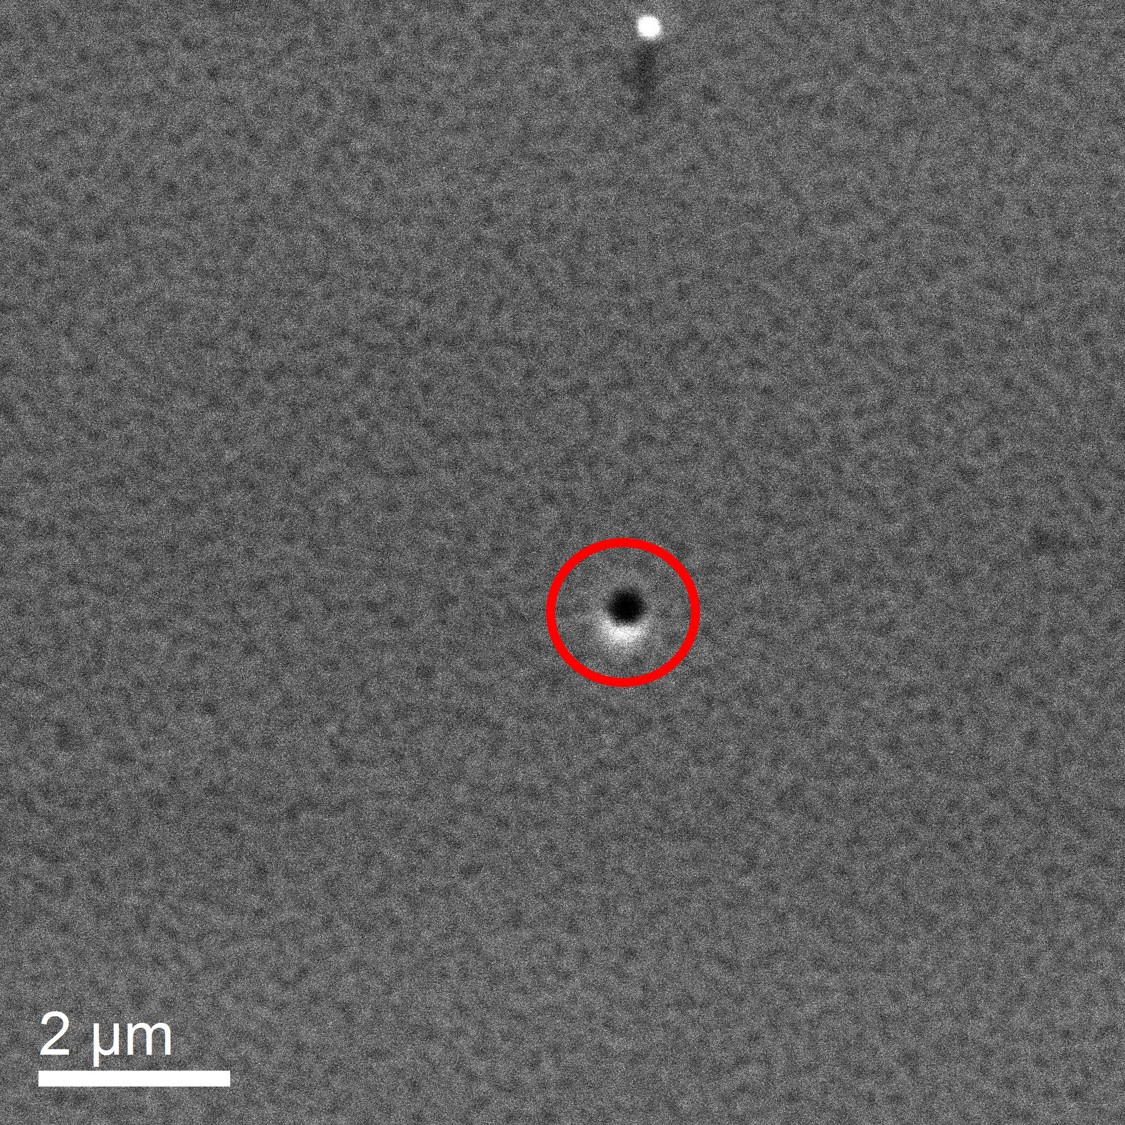
\includegraphics[width=0.7\linewidth]{Figs/Ch3/5608sem}
		\caption{}
		
	\end{subfigure}%
	\hspace*{0.5cm}
	\begin{subfigure}[b]{0.48\textwidth}
		\centering
		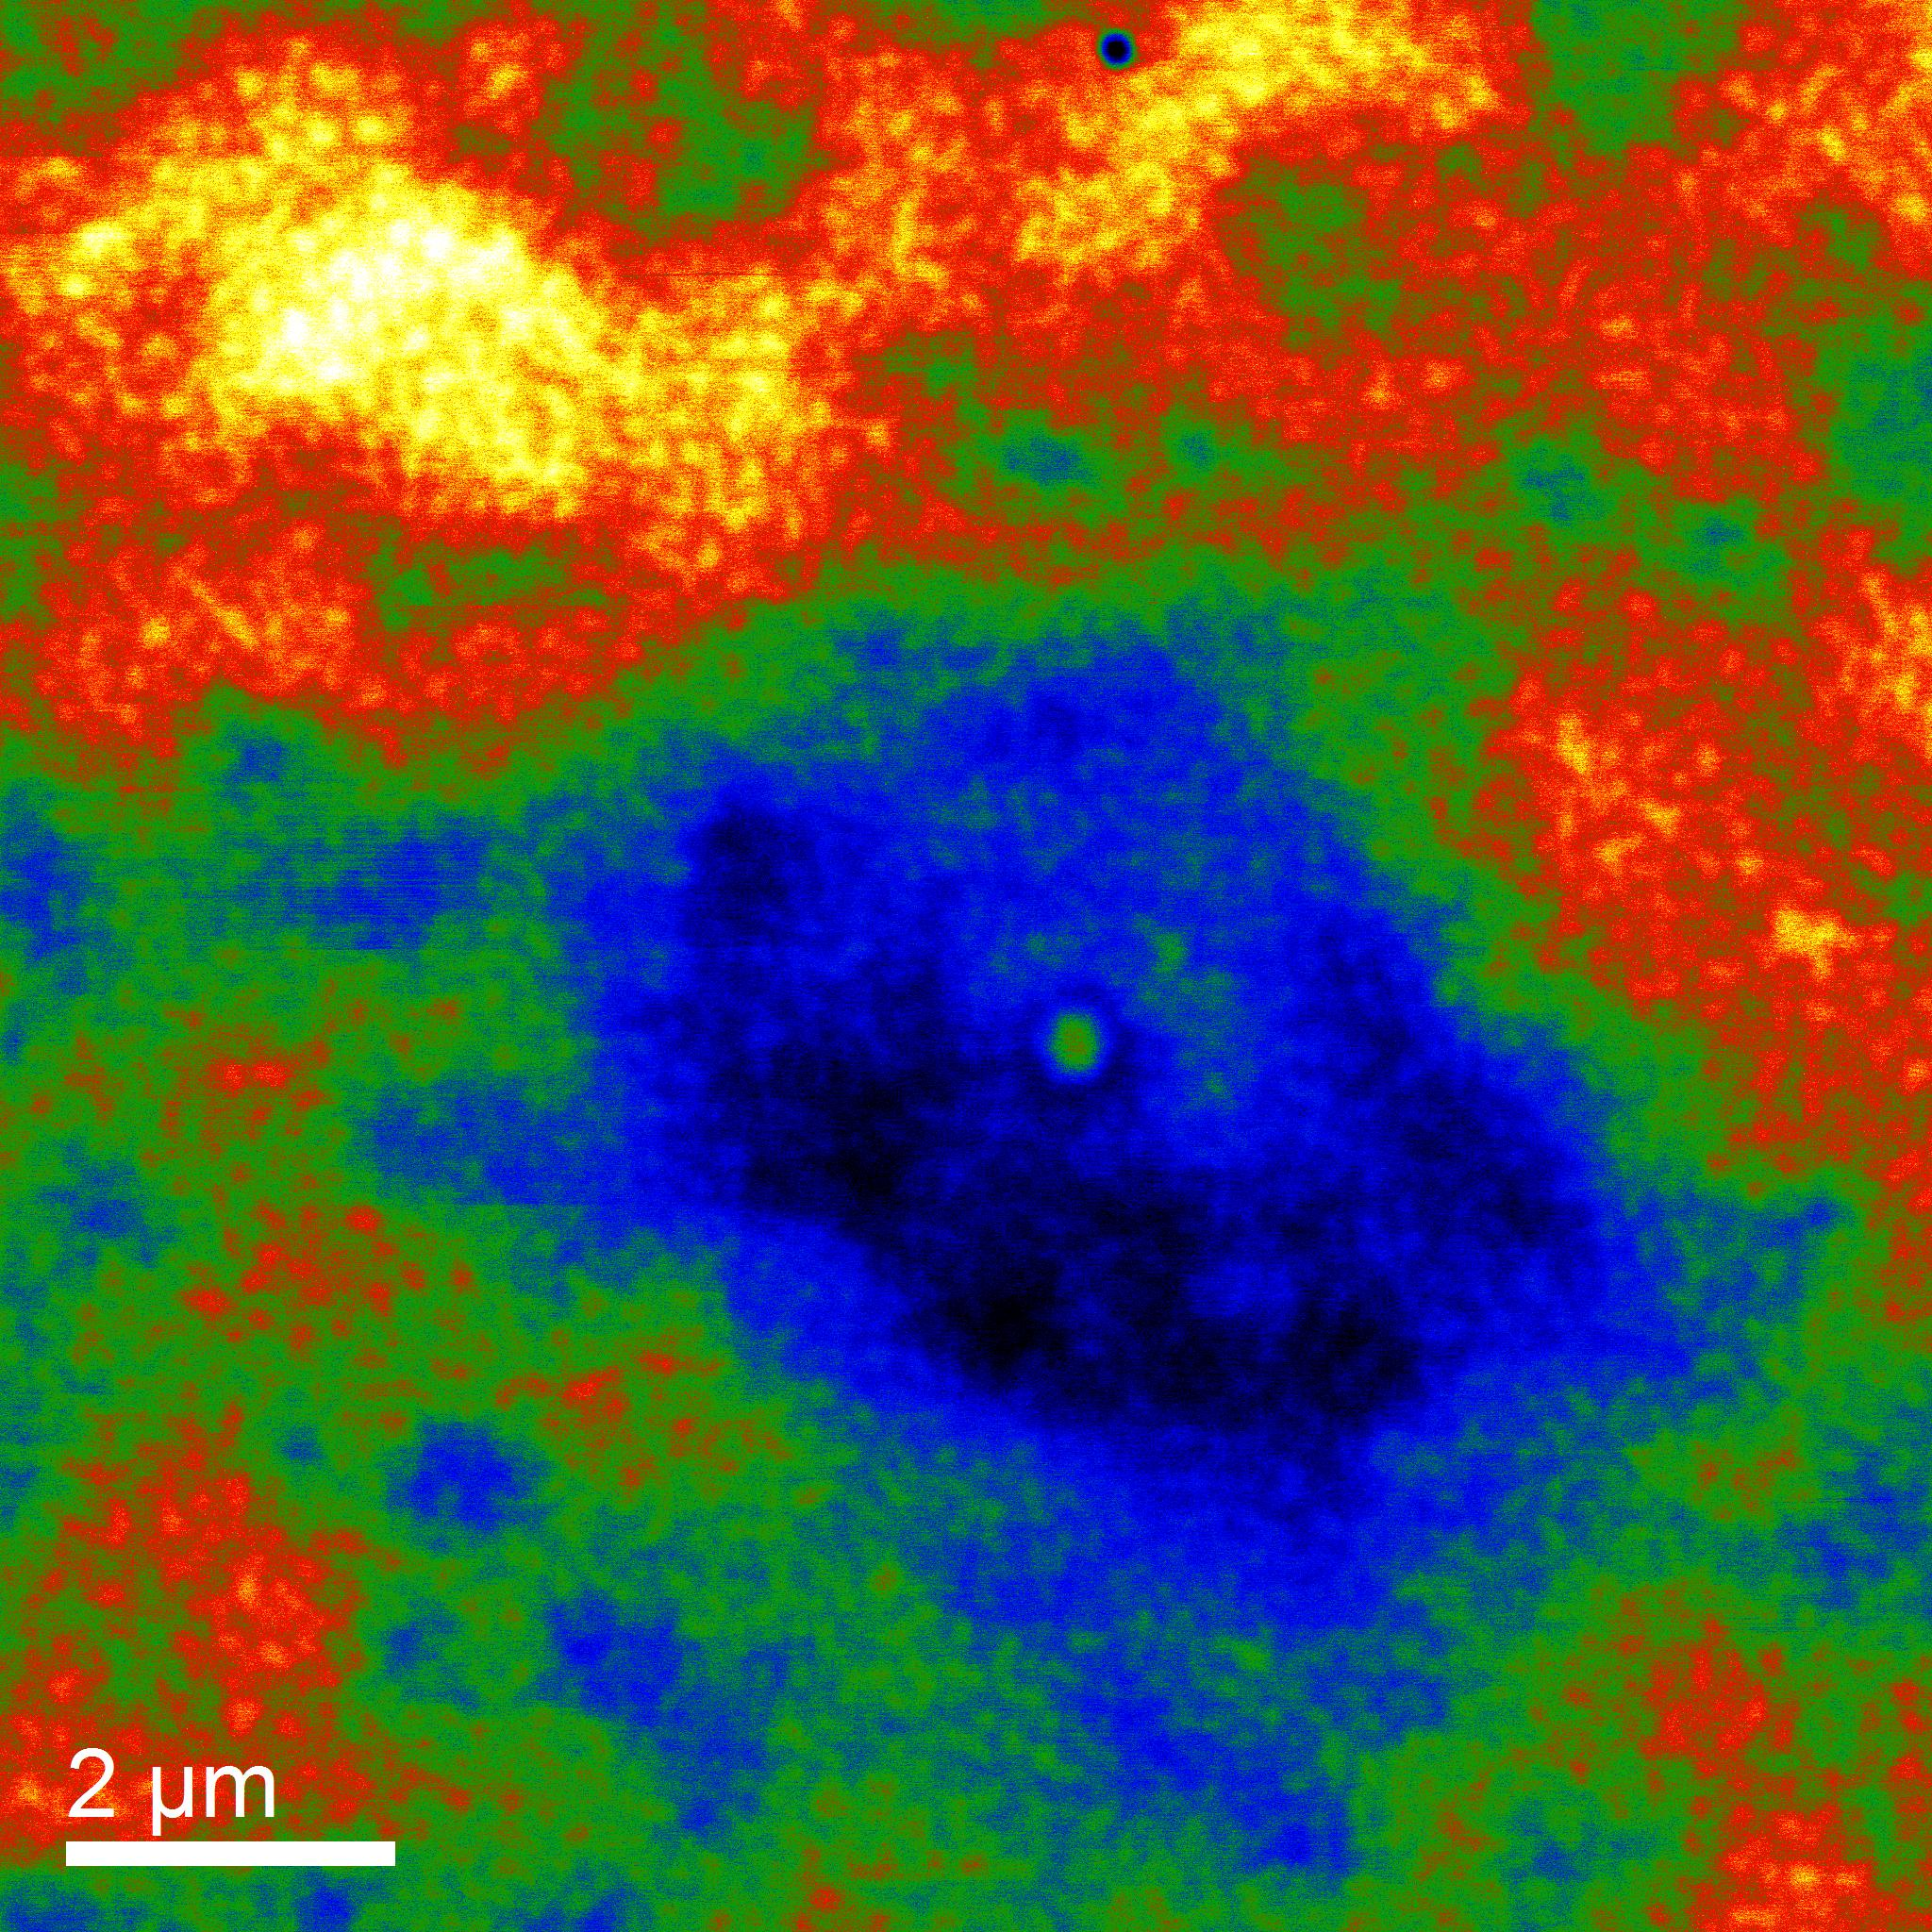
\includegraphics[width=0.7\linewidth]{Figs/Ch3/5608panCL}
		\caption{}
	\end{subfigure}%
	
	\caption{a) SEM micrograph and b) pan-CL image of an inhomogeneity in C5608A. The pan-CL image utilises a temperature scale (blue = low, red = high).}
	\label{5608-SEM-CL}
\end{figure}
\FloatBarrier

A hyperspectral CL map of 2 $\times$ 2 $\mu m^{2}$ was taken to examine the emissive properties of the defect in more detail. Fig.\ref{11-CL}.a. shows that as expected, the region close to the hexagonal defect exhibits low CL intensity. Interestingly, the defect also shows extremely low-energy emission relative to the background, most likely due to defect-related yellow band emission \cite{Lyons2010}.

\begin{figure}[h]
	
	\begin{subfigure}[b]{0.48\textwidth}
		\centering
		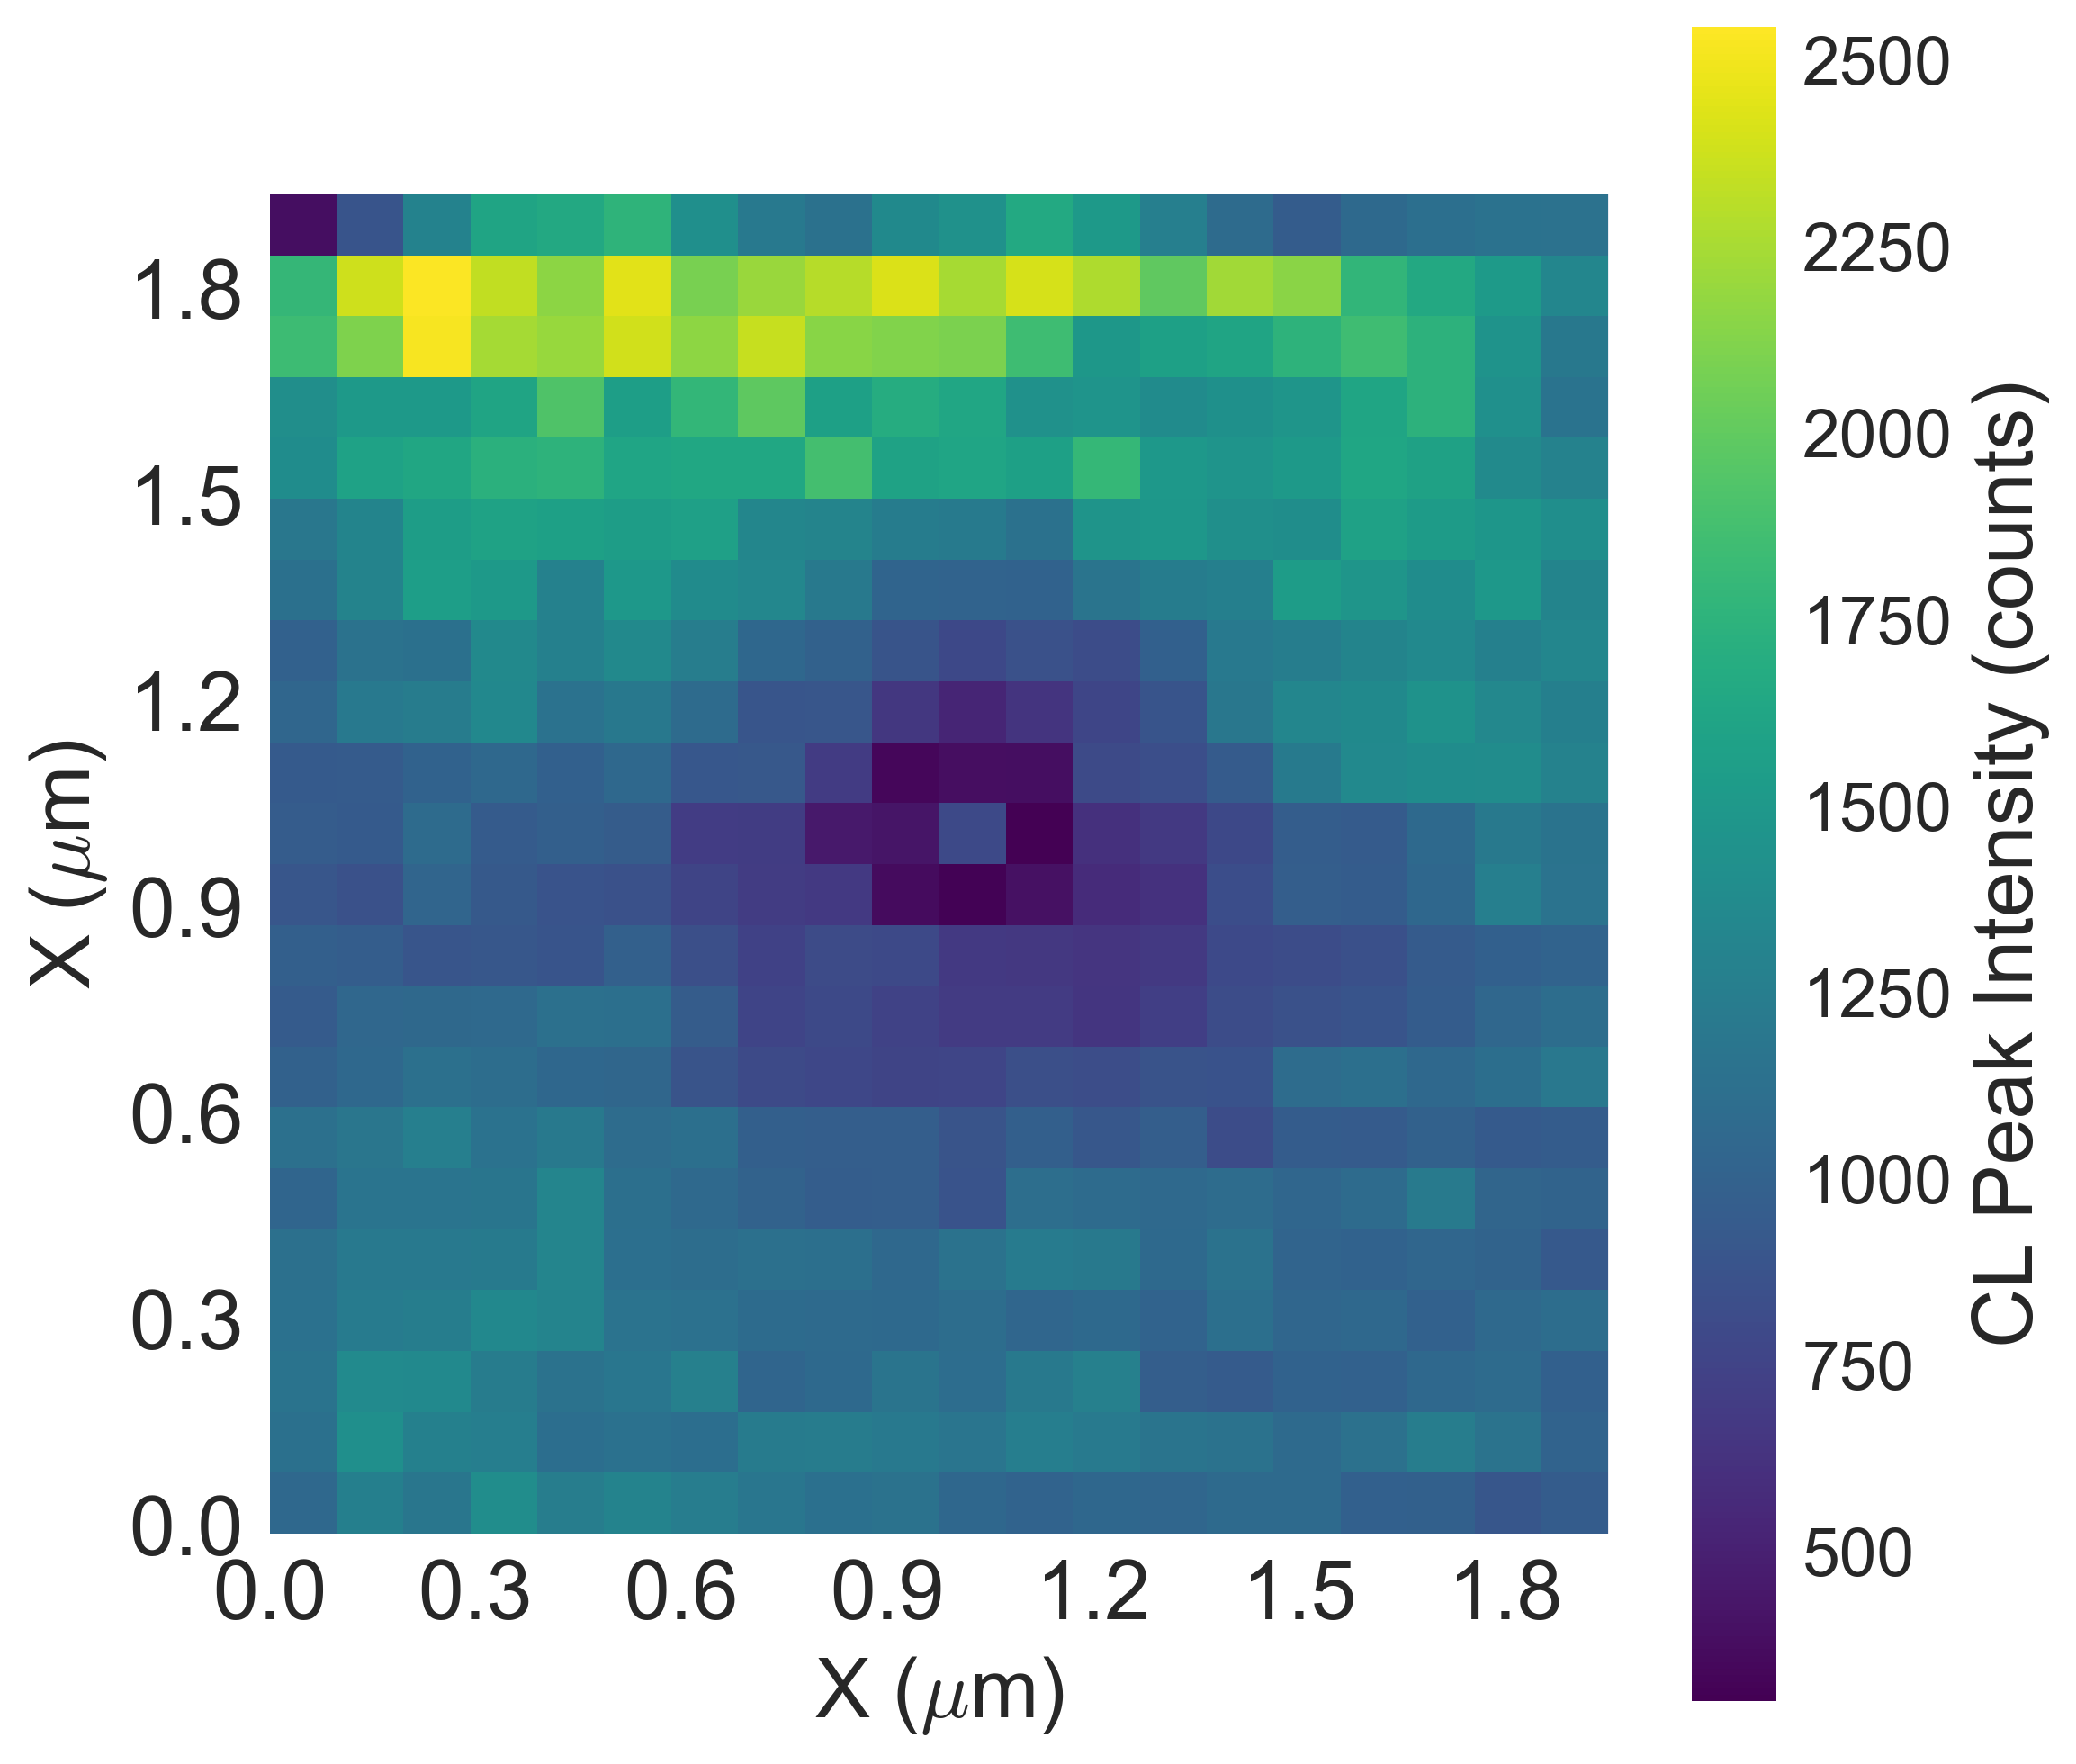
\includegraphics[width=1\linewidth]{Figs/Ch3/11-peak}
		\caption{}
		
	\end{subfigure}%
	\hspace*{0.5cm}
	\begin{subfigure}[b]{0.48\textwidth}
		\centering
		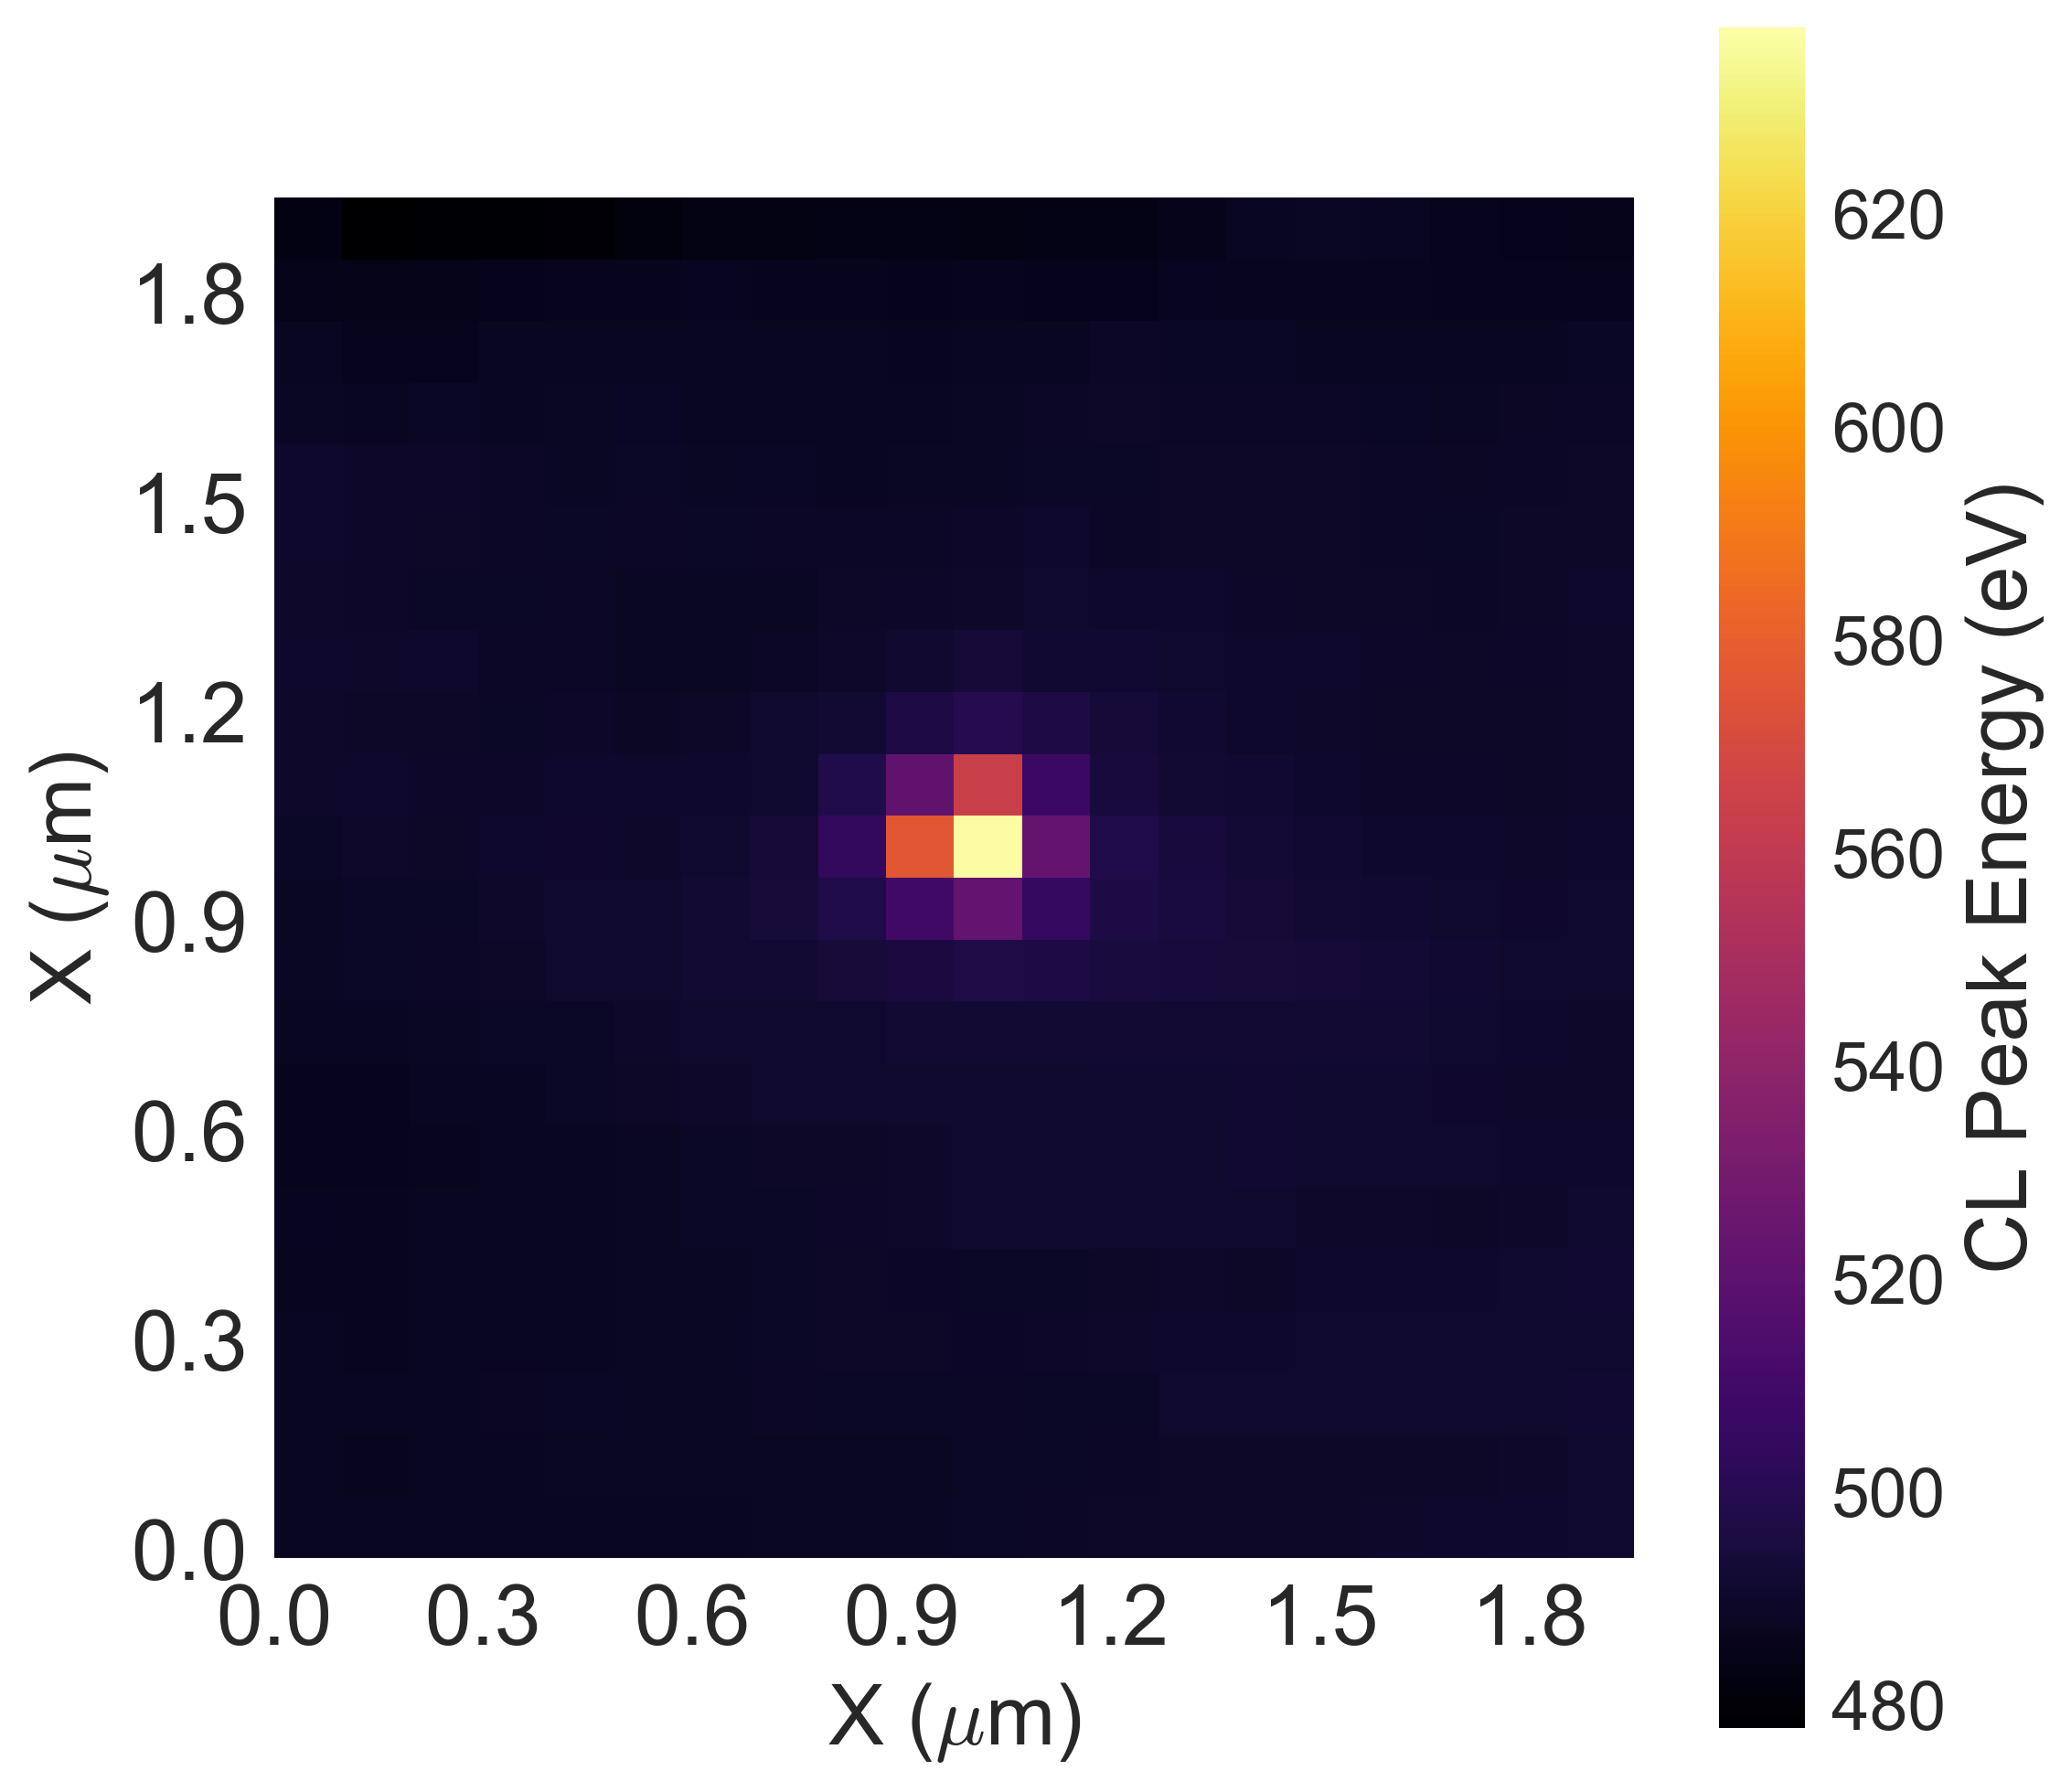
\includegraphics[width=1\linewidth]{Figs/Ch3/11-centre}
		\caption{}
	\end{subfigure}%
	
	\caption{a) CL peak intensity and b) CL peak energy for the feature shown in Fig.\ref{5608-SEM-CL}}
	\label{11-CL}
\end{figure}
\FloatBarrier

\subsection{Hexagonal Defect Structure}

The structure of the hexagonal defects found at the centre of the inhomogeneities was examined following their detection using SEM-CL. 

\subsubsection{Scanning Electron Microscopy}
In order to achieve a higher resolution in examining the defects via SEM, an FEI Helios Nanolab 650 SEM/FIB with a schottky FEG at 5 kV and through lens detector (TLD) was used to perform high resolution SEM imaging. This is shown in Fig. \ref{sem-pit}.

\begin{figure}[!ht]
	\centering
	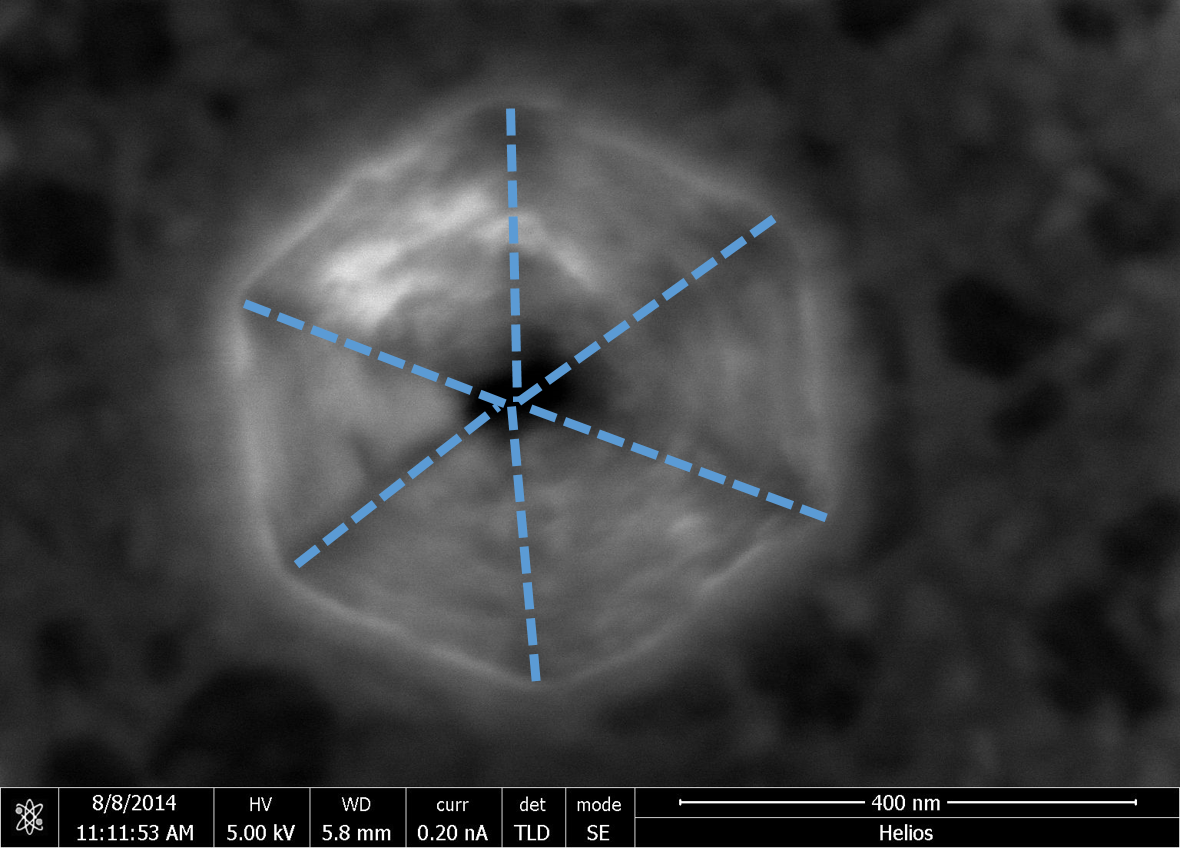
\includegraphics[width=0.8\textwidth]{Figs/Ch3/sem-pit.png}
	\caption[h] {High-resolution SEM image of a hexagonal defect located at the centre of an inhomogeneity in the EL. The vertices of the facets are delineated by dashed lines.}
	\label{sem-pit}
\end{figure}
\FloatBarrier 

Most hexagonal defects located at the centre of the inhomogeneities fell within the 200-600 nm range, with some exceedingly large defects reaching up to 1 $\mu$m in size. This is rather uncommon for hexagonal defects in III-nitrides, as the lateral size of hexagonal defects is typically sub-100 nm \cite{Oliver2006a,Tsai2007}.

\subsubsection{Atomic Force Microscopy}
The topography of the hexagonal defect was studied by AFM performed on a Veeco Dimension 3100 with RTESP tips with a nominal radius of 8 nm in intermittent contact mode. The defect shown in the SEM micrograph in Fig.\ref{sem-pit} is shown below in the AFM image.

\begin{figure}[!ht]
	\centering
	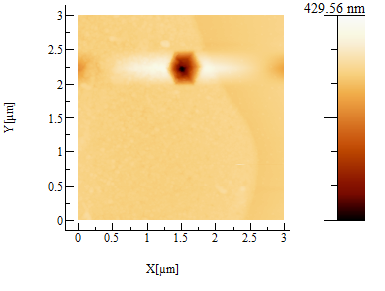
\includegraphics[width=0.7\textwidth]{Figs/Ch3/AFM.png}
	\caption[h] {AFM image of the hexagonal defect.}
	\label{afm-pit}
\end{figure}
\FloatBarrier 

By taking a topography profile across the hexagonal defect, we can resolve the depth of the defect as well as the slope of the facets.

\begin{figure}[!ht]
	\centering
	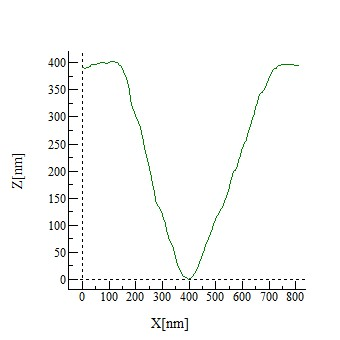
\includegraphics[width=0.5\textwidth]{Figs/Ch3/profile}
	\caption[h] {Profile taken across the defect shown in Fig.\ref{afm-pit}}
	\label{profile}
\end{figure}
\FloatBarrier 

\subsubsection{TEM Lamella preparation}

Preparation of TEM lamellae for the analysis of the defects requires some additional steps due to site-specific nature of the experiment. Standard FIB/SEM sample preparation methods simply require a 2 $\mu$m thick wedge of the sample to be extracted and thinned down to a thickness of 100-200 nm for TEM experiments. However, analysis of the defect and any associated dislocations which may be present at the apex of the inverted pyramidal shape \cite{Watanabe2003,Shiojiri2006} requires thinning to be performed in an extremely controlled manner. A method devised by Thomas O'Hanlon at the Cambridge Centre for Gallium Nitride was utilised to perform high-precision site specific TEM sample preparation shown in Fig.\ref{FIBprep}. A 'marker layer' consisting of a cross intersecting the apex of the defect is deposited using the electron beam, thus allowing for little damage to the unprotected sample and a higher deposition resolution than the ion beam. Following this a protective layer is then deposited using the ion beam, and a standard dual-beam lift-out method is used to extract the wedge of sample containing the defect. 

\begin{figure}[!ht]
	\centering
	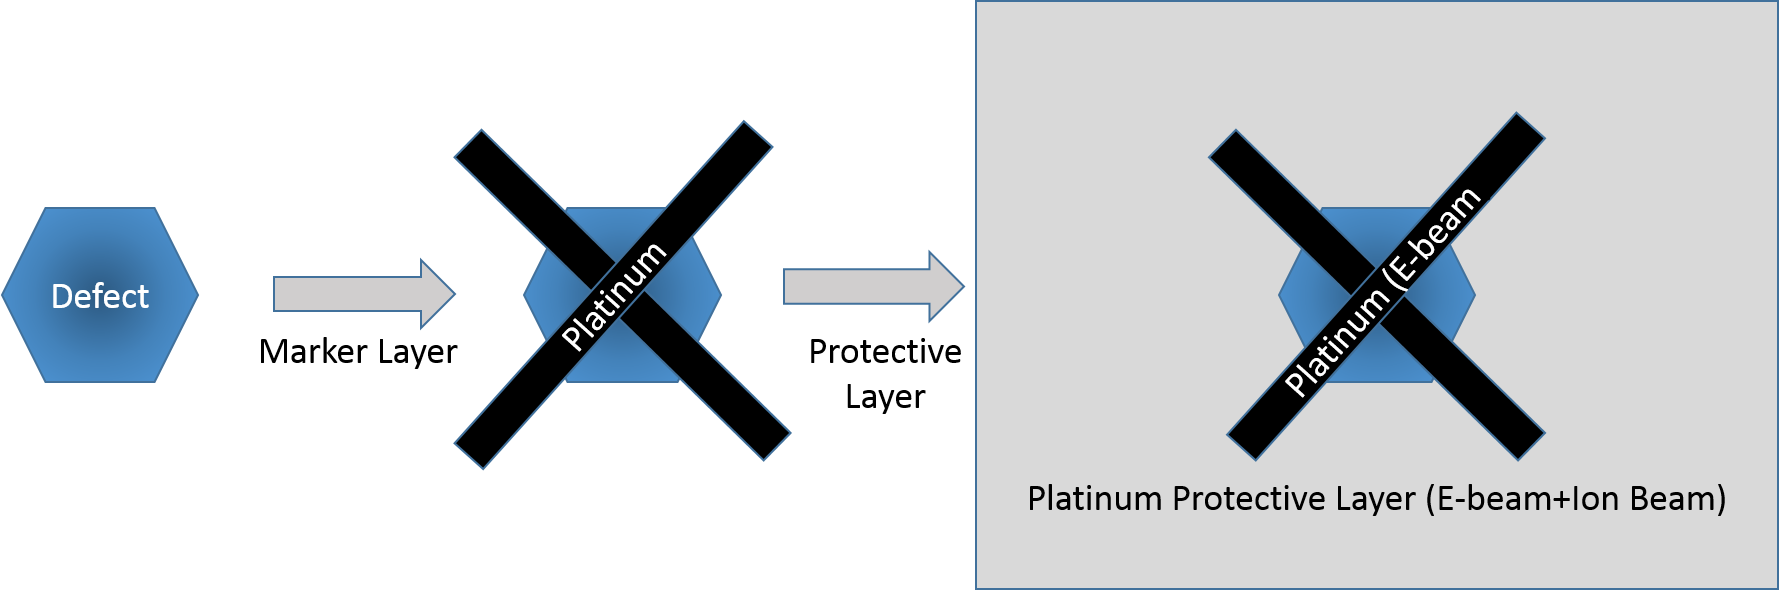
\includegraphics[width=1\textwidth]{Figs/Ch3/FIB-spot}
	\caption[h] {Marker layer deposition for high precision TEM sample preparation.}
	\label{FIBprep}
\end{figure}
\FloatBarrier 

The purpose of the marker layer is guide the sample thinning process. The electron beam deposited platinum provides contrast against both the sample and the ion-beam platinum in the SEM image. As the sample is imaged in cross-section during the thinning process, the distance between the marker layer 'ends' is an indicator of the proximity to the defect apex. As the defect apex is reached during the thinning process, the two marker stripes should merge into one at the intersection of the cross, as shown in Fig.\ref{FIBloc}.

\begin{figure}[!ht]
	\centering
	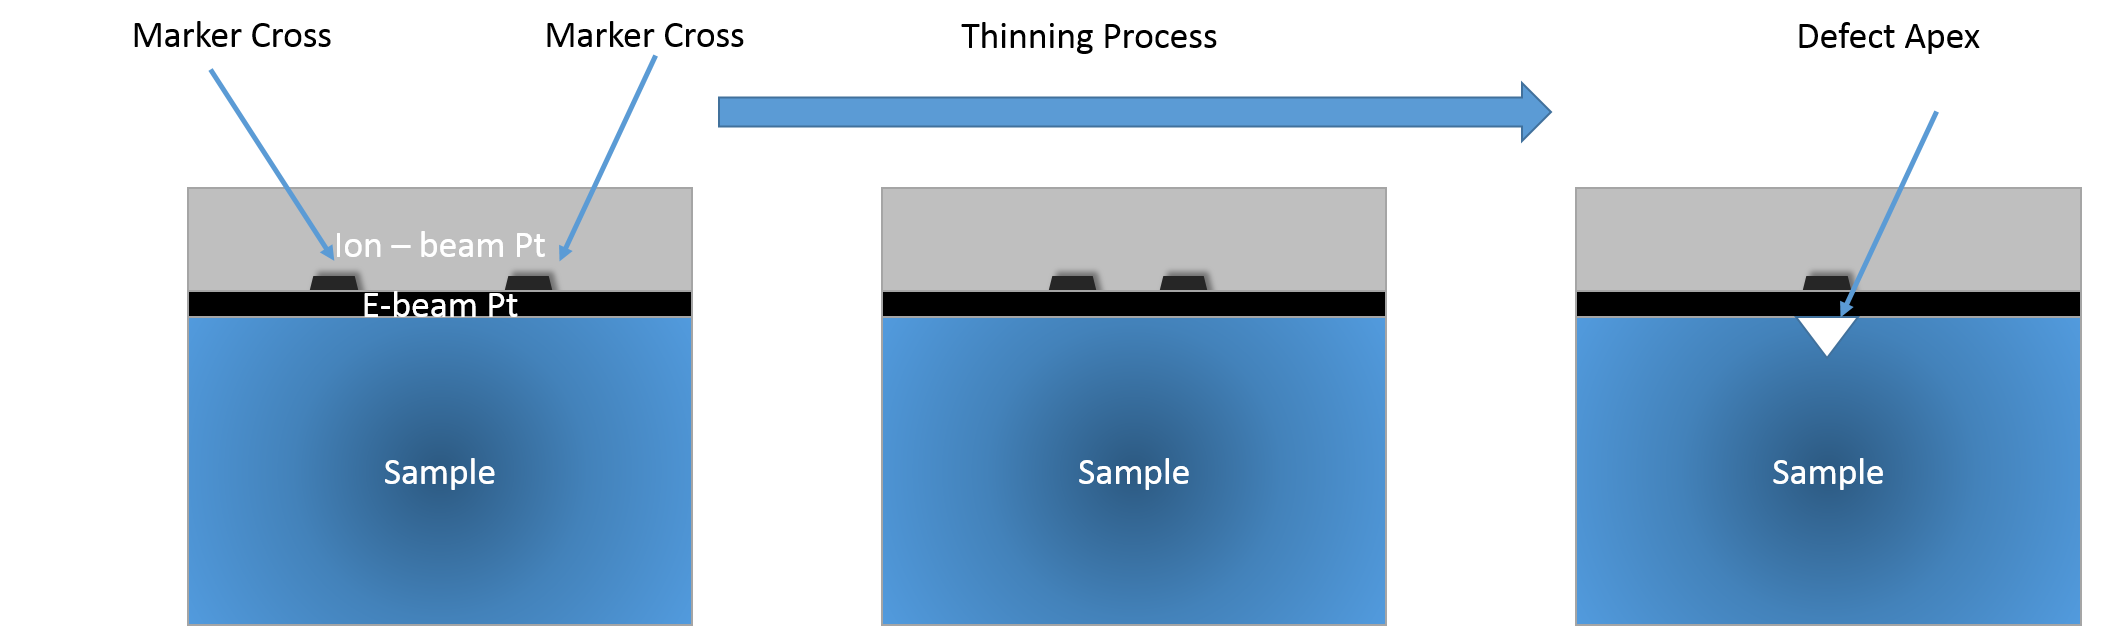
\includegraphics[width=1\textwidth]{Figs/Ch3/FIB-loc-diagram}
	\caption[h] {Marker layer deposition for high precision TEM sample preparation.}
	\label{FIBloc}
\end{figure}
\FloatBarrier 

A successfully thinned sample is shown in Fig.\ref{thinned}.

\begin{figure}[h]
	\centering
	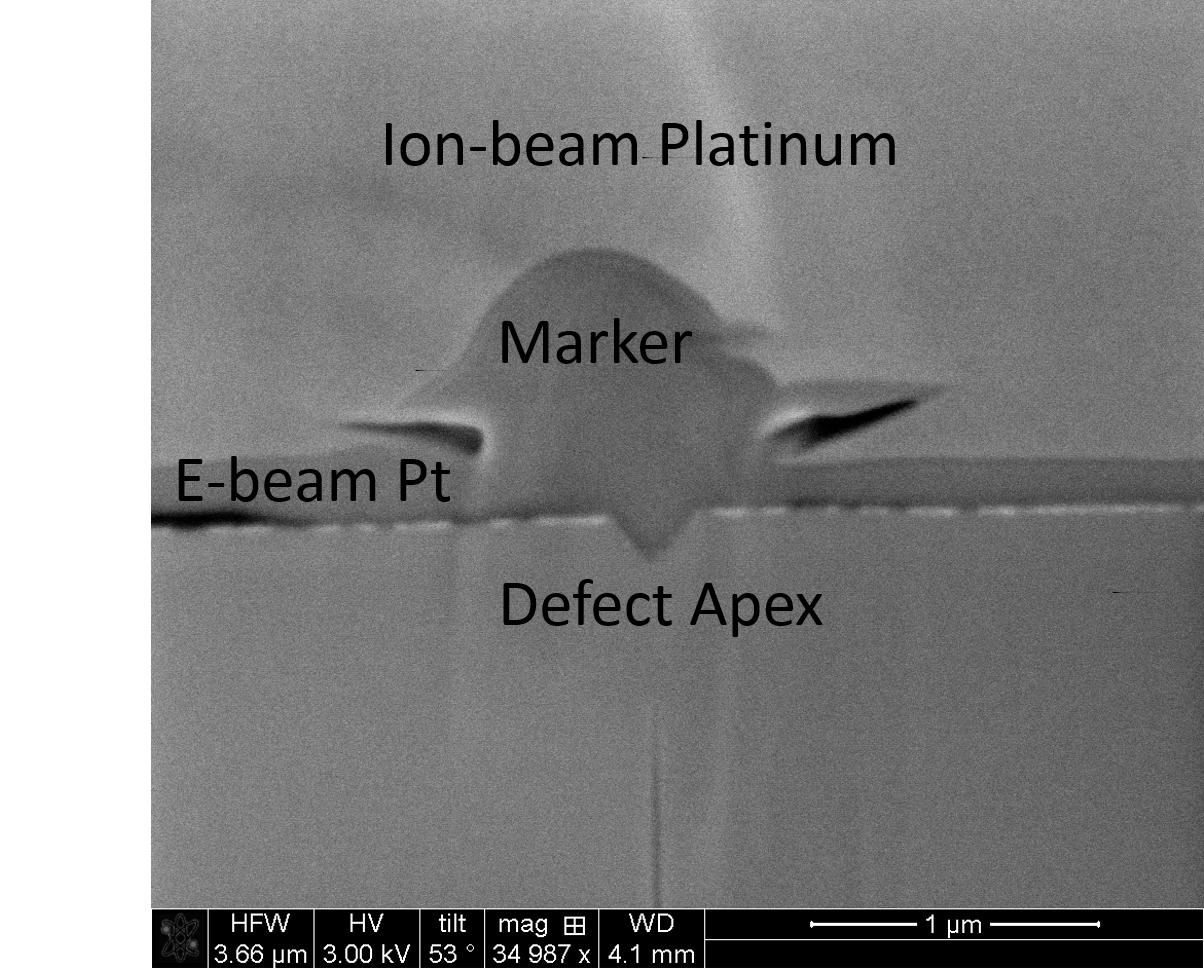
\includegraphics[width=0.6\textwidth]{Figs/Ch3/thinned}
	\caption[h] {SEM image of a prepared TEM lamella showing the marker position and defect apex.}
	\label{thinned}
\end{figure}
\FloatBarrier 


\subsubsection{Transmission Electron Microscopy}

The site-specific TEM lamella prepared using the dual-beam methods, shown in Fig.\ref{thinned}, was studied by HAADF-STEM performed on an FEI Osiris microscope with an extreme-FEG (X-FEG) \nomenclature[z-X-FEG]{X-FEG}{Extreme Field-Emission Gun} at 200 kV. HAADF-STEM imaging of the defect reveals it originates below the MQW stack, a possible explanation for the large size of the hexagonal defects relative to those reported in literature \cite{Hangleiter2005,Tsai2007,Oliver2006a}. 

\begin{figure}[h]
	\centering
	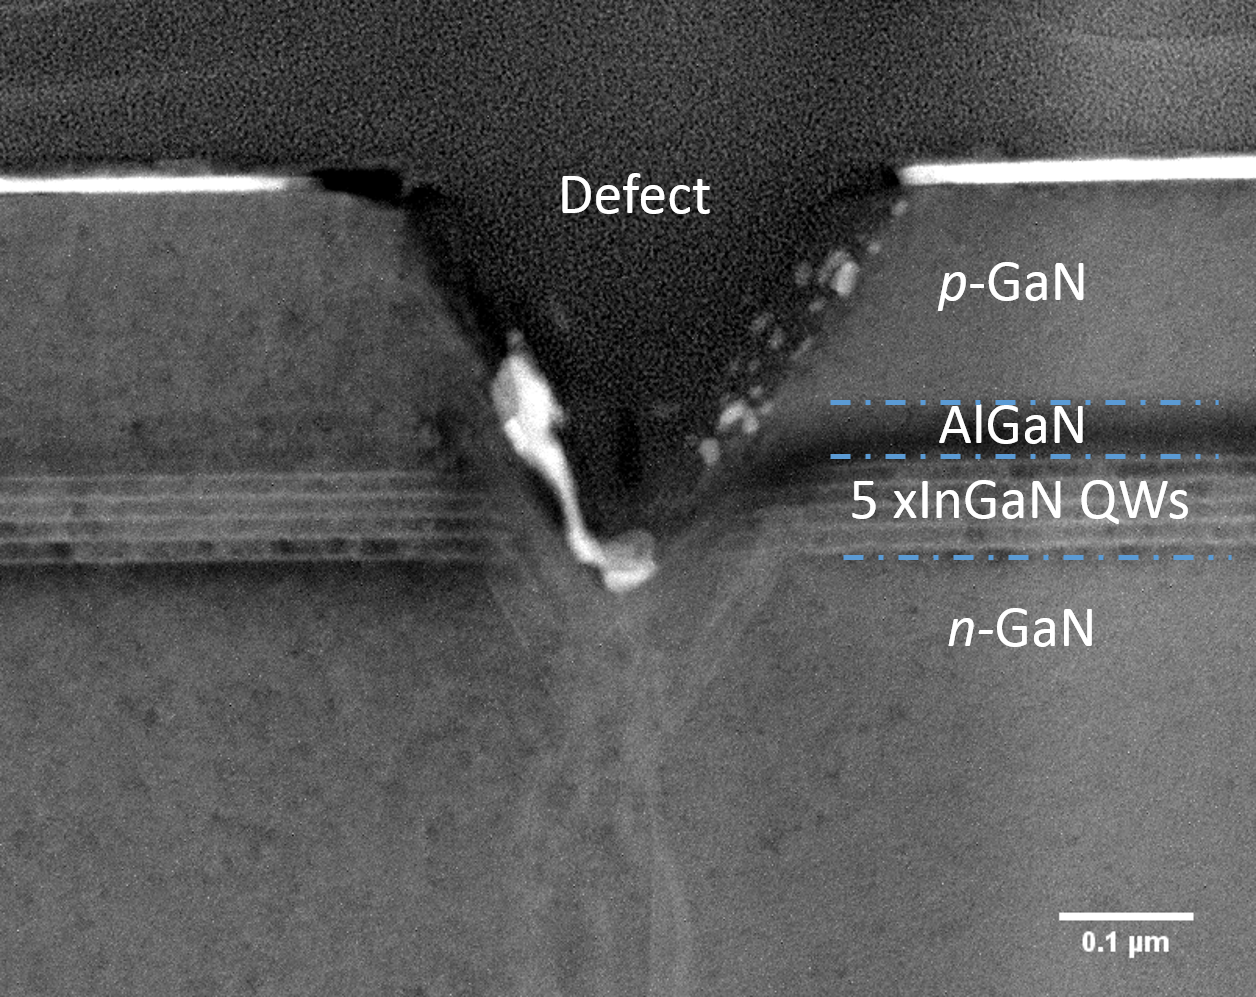
\includegraphics[width=0.6\textwidth]{Figs/Ch3/STEM-spot}
	\caption[h] {HAADF-STEM image of a prepared TEM lamella showing defect interrupting the QW stack.}
	\label{STEM-spot}
\end{figure}
\FloatBarrier 

The composition of the MQW stack adjacent to the region occupied by the defect was studied using EDX-STEM, where the characteristic X-rays emitted by the sample were recorded by four silicon drift detectors which form a solid angle greater than 0.9 sr. Cliff-Lorimer analysis of the aluminium, gallium and indium was performed using HyperSpy in order to quantify the ternary alloy compositions as shown in Fig.\ref{EDXspot}

\begin{figure}[h]
	\begin{subfigure}[b]{0.48\textwidth}
	\centering
		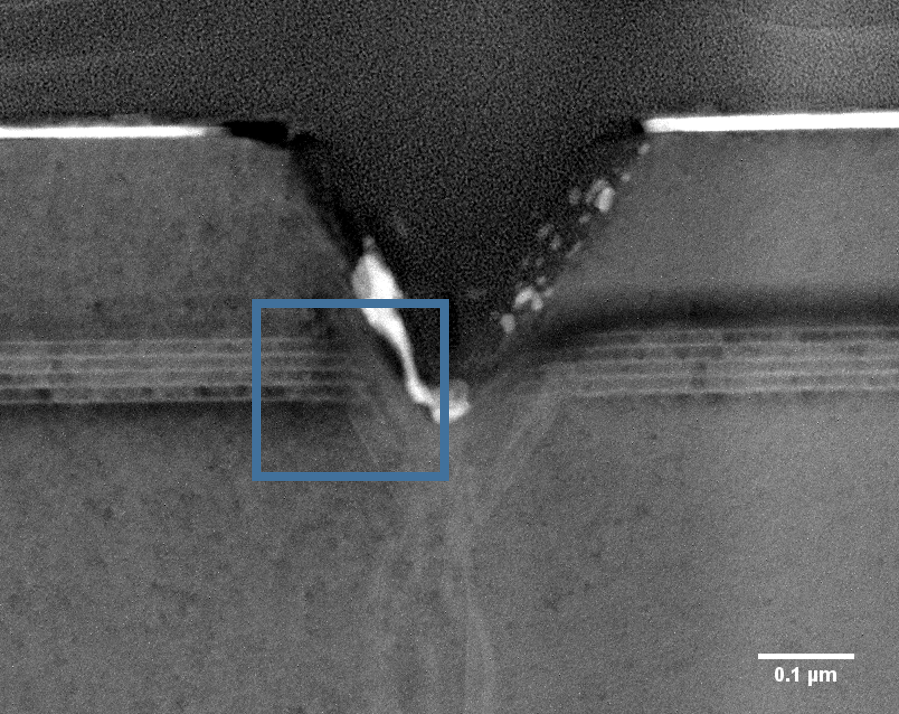
\includegraphics[width=1\linewidth]{Figs/Ch3/EDStarget}
		\caption{}
	\end{subfigure}%
	\hspace*\fill
	\begin{subfigure}[b]{0.48\textwidth}
		\centering
		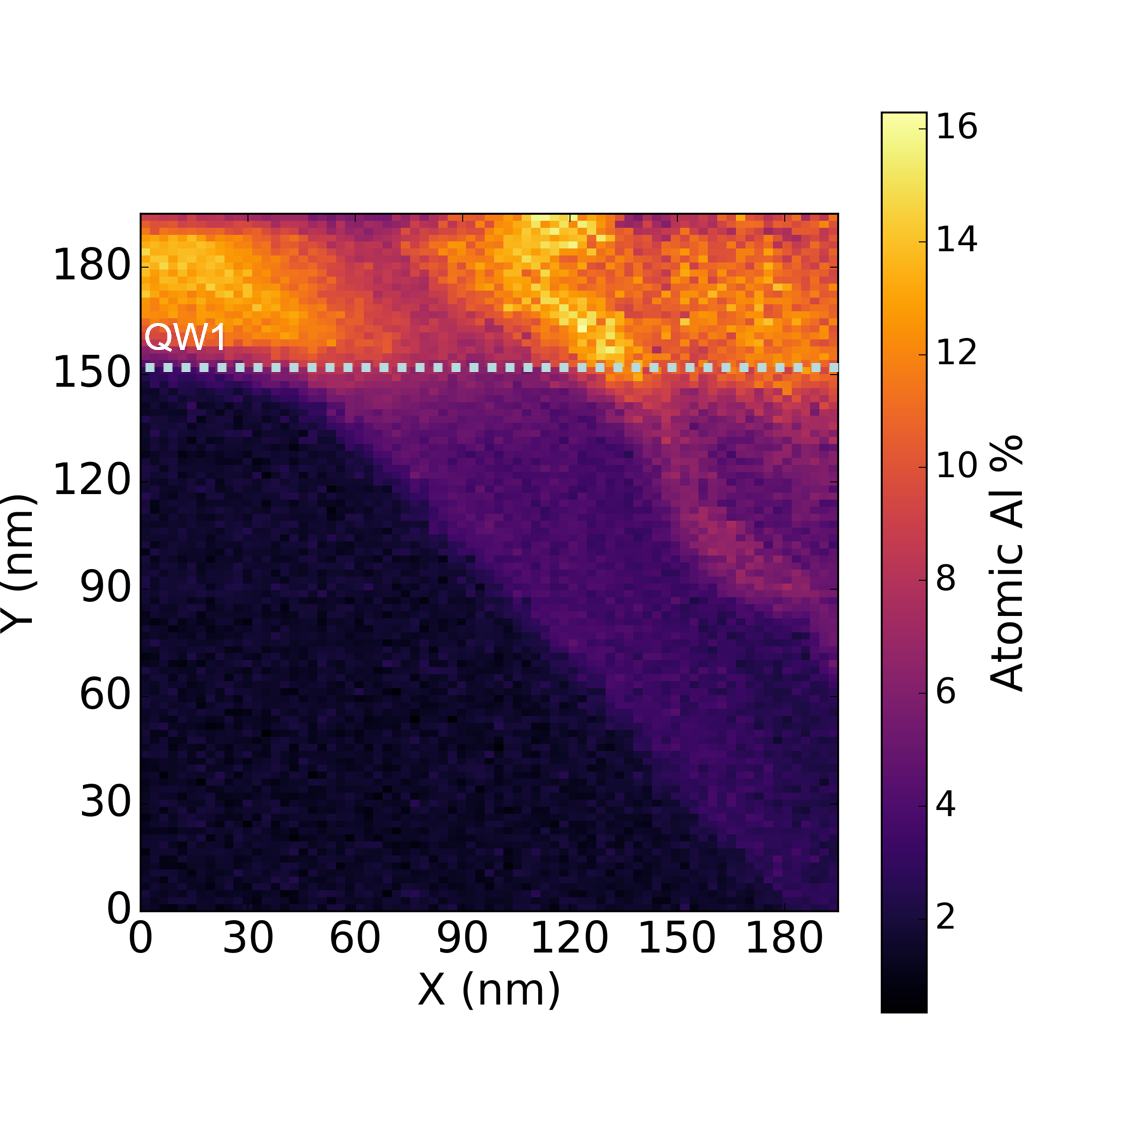
\includegraphics[width=1\linewidth]{Figs/Ch3/AtomicAl}
		\caption{}		
	\end{subfigure}%
	
	\medskip
	\begin{subfigure}[b]{0.48\textwidth}
		\centering
		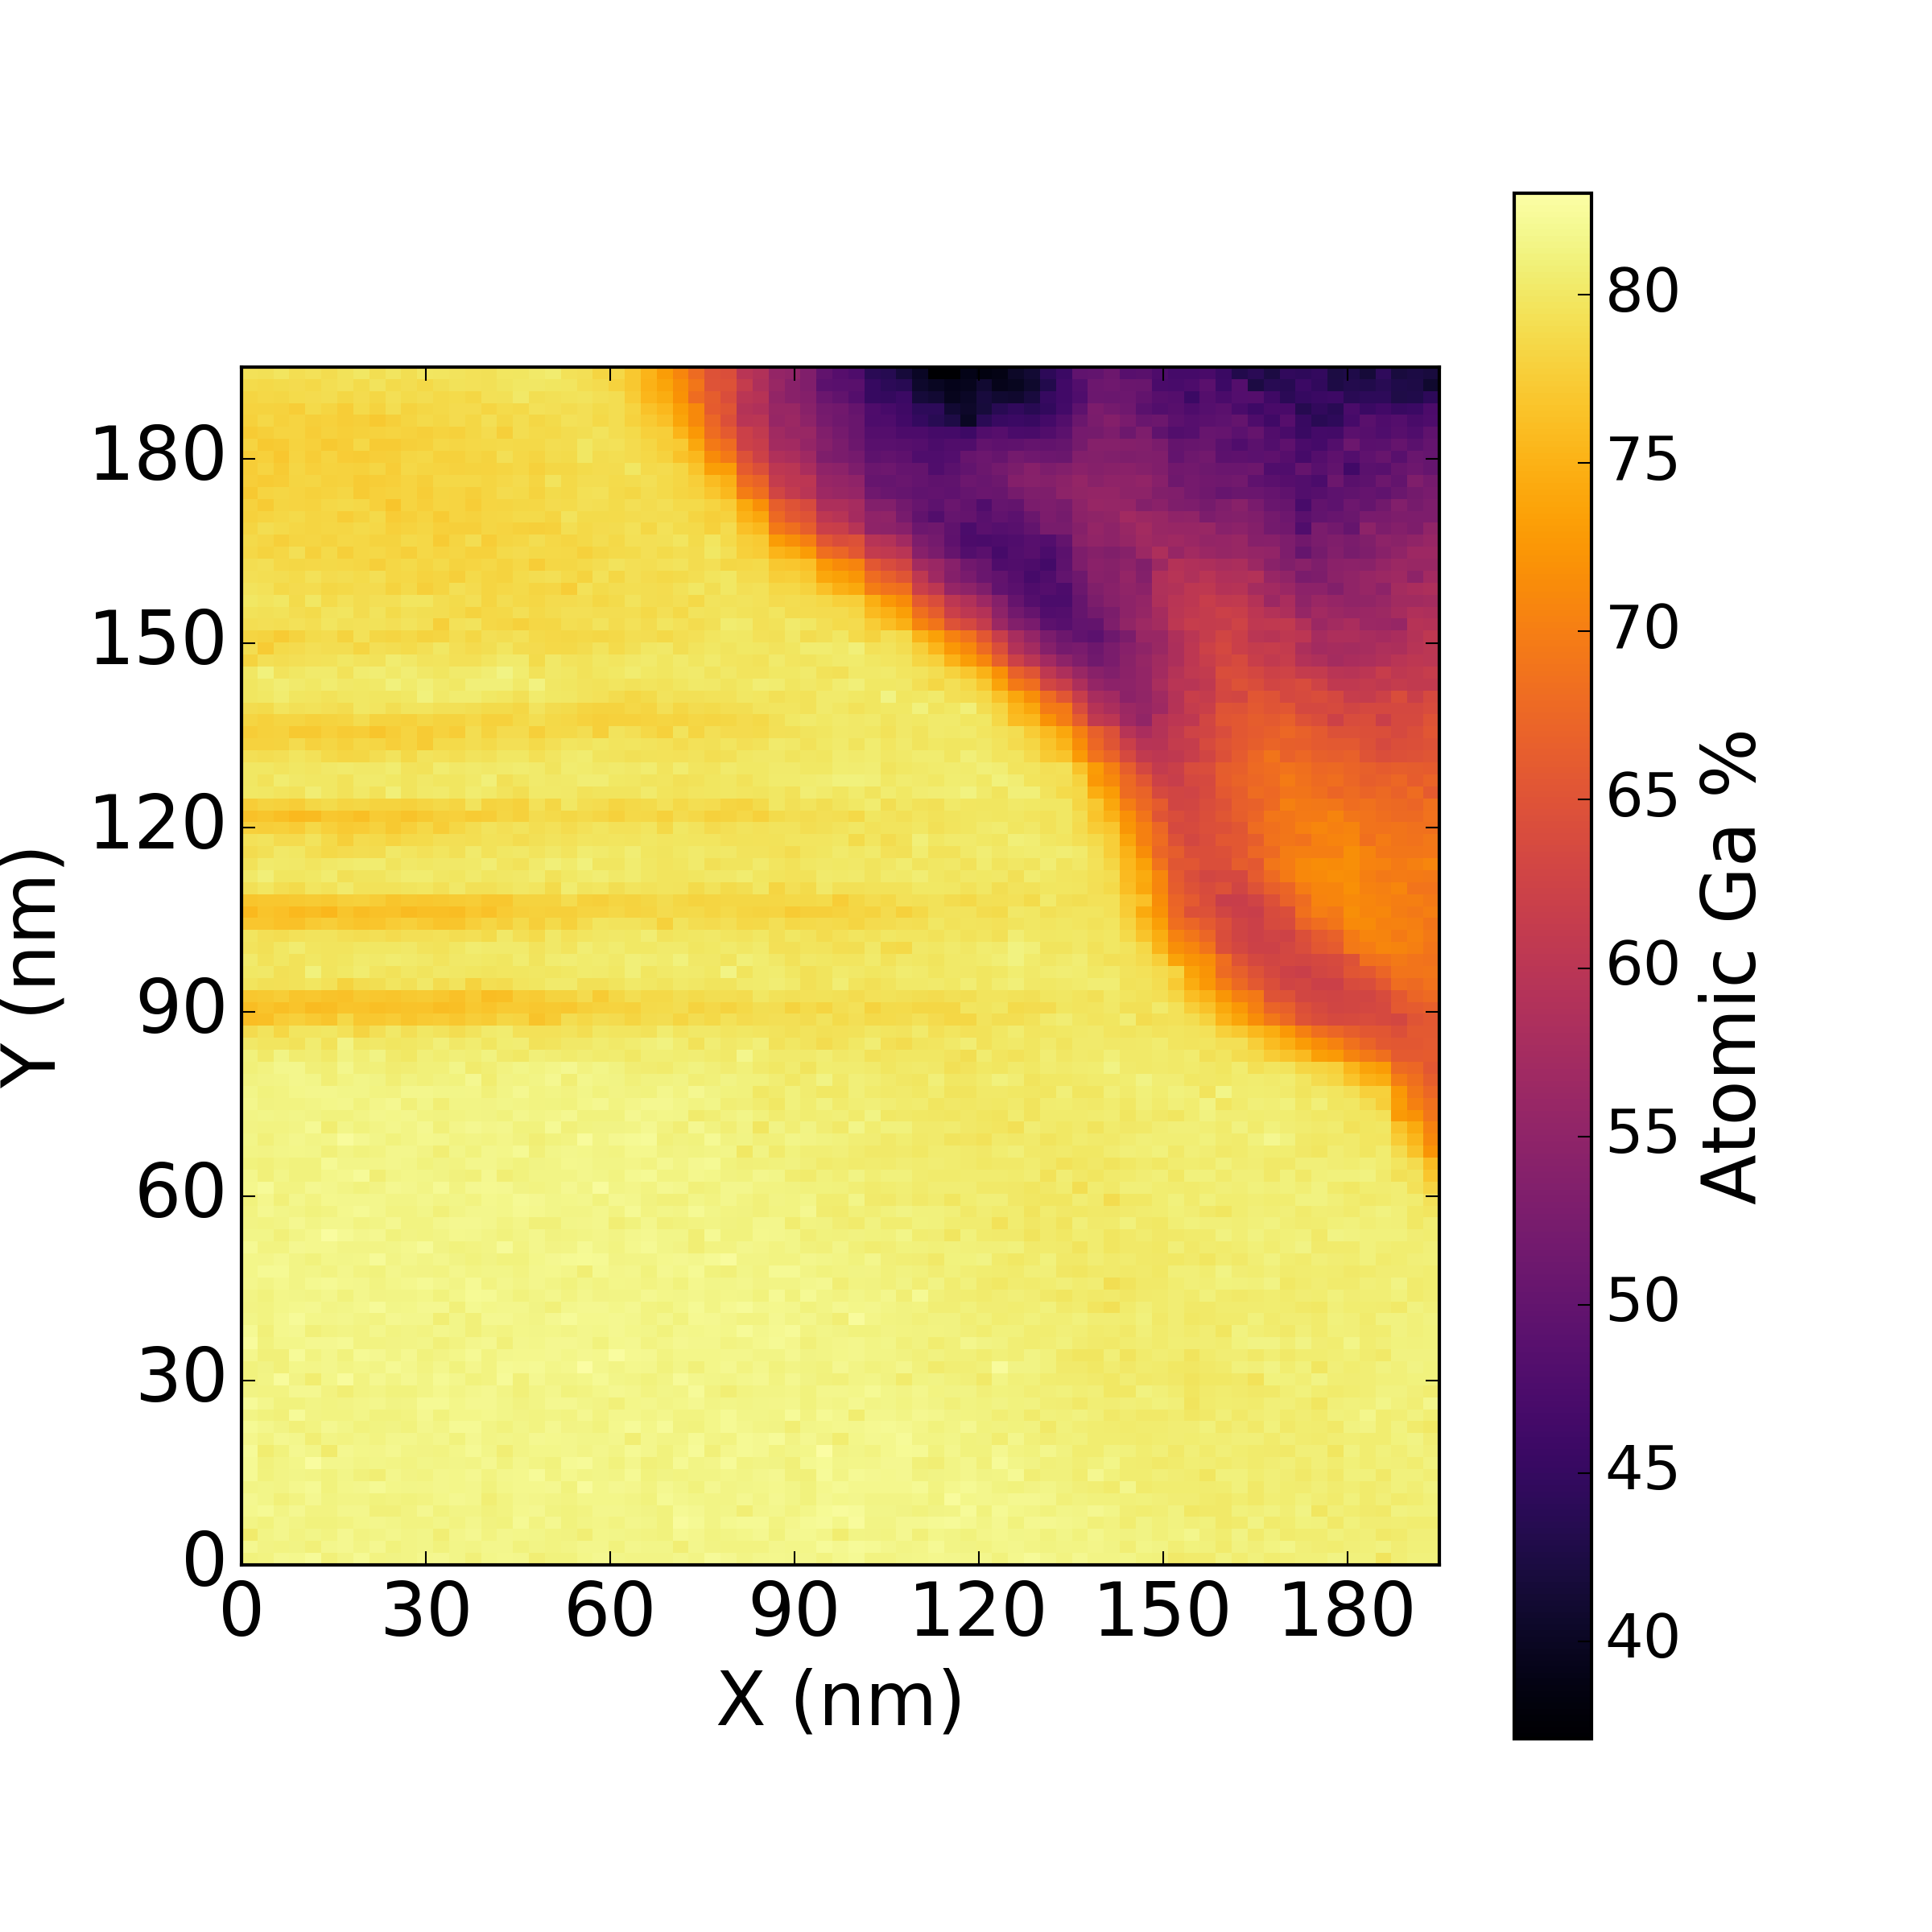
\includegraphics[width=1\linewidth]{Figs/Ch3/AtomicGa}
		\caption{}
	\end{subfigure}%
	\hspace*\fill
	\begin{subfigure}[b]{0.48\textwidth}
		\centering
		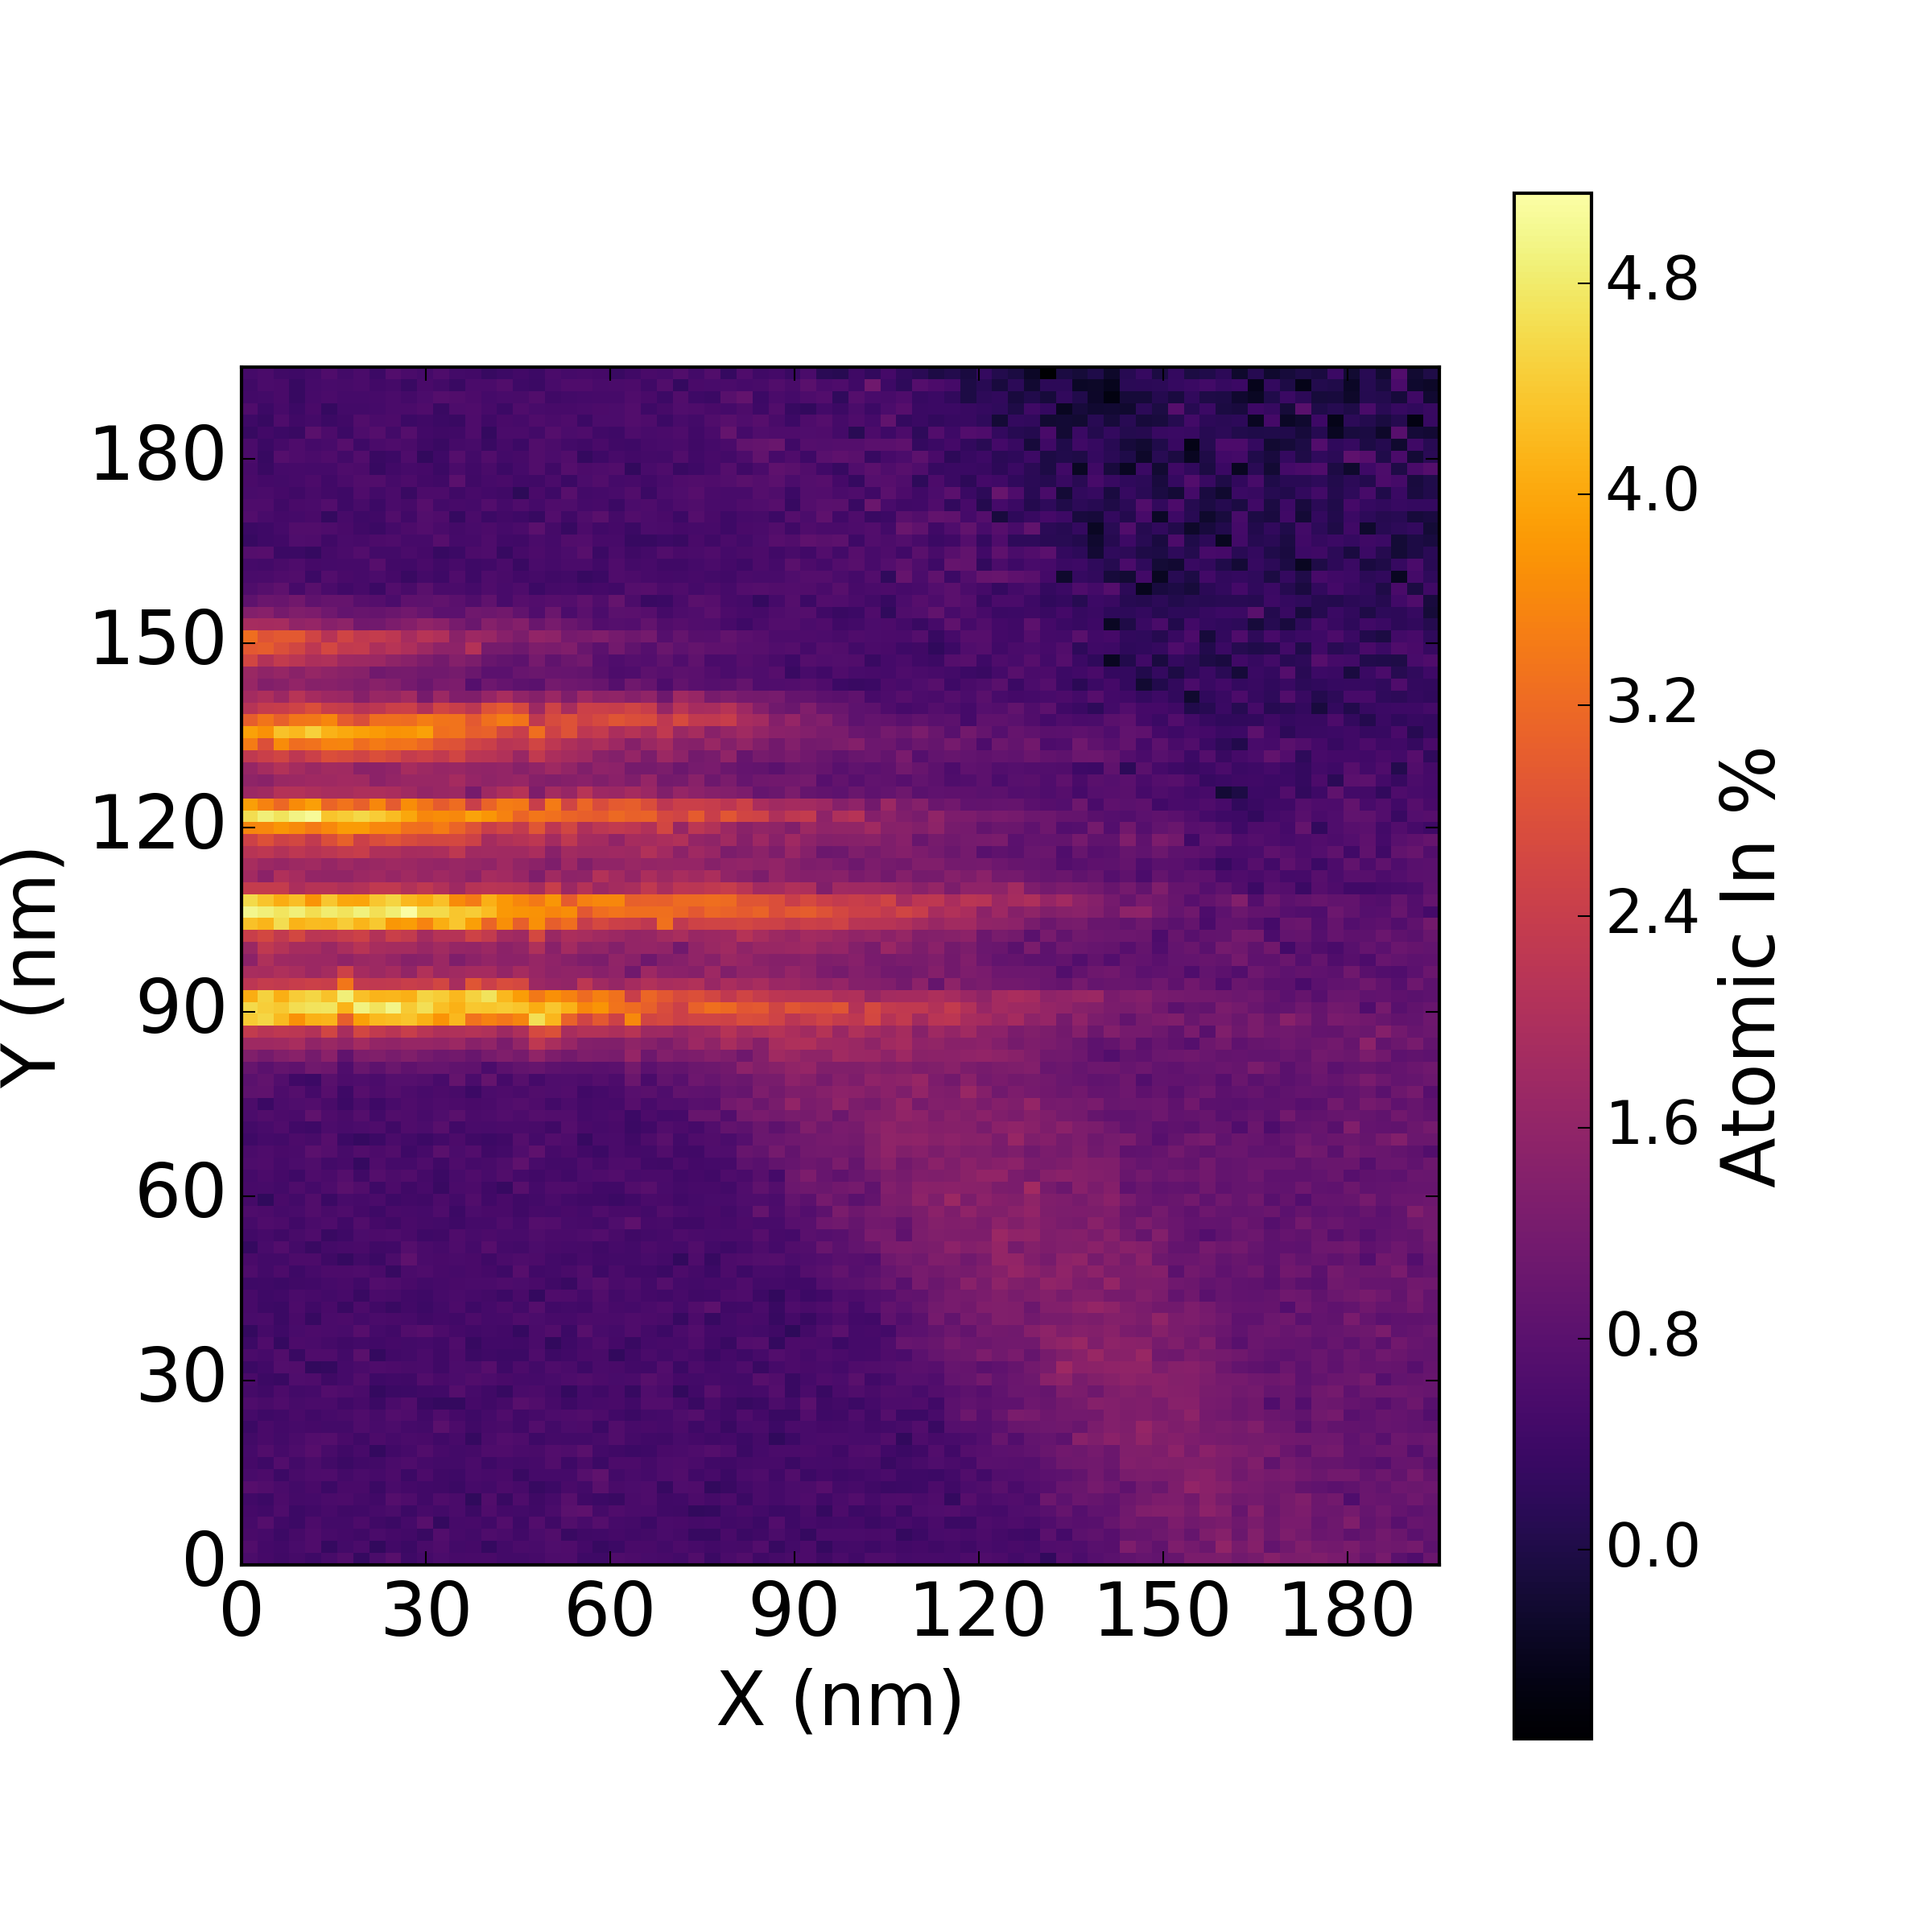
\includegraphics[width=1\linewidth]{Figs/Ch3/AtomicIn}
		\caption{}		
	\end{subfigure}%
	

	\caption{Quantification of the ternary alloy compositions: a) HAADF-STEM image showing the region examined by EDX (blue box) b) aluminium atomic percentage, c) gallium atomic percentage and d) indium atomic percentage.}
	\label{EDXspot}
\end{figure}
\FloatBarrier 
The EDS analysis shows the disruption of the QW stack by the defect, as evidenced by the apparent termination of the QW In signal in Fig.\ref{EDXspot}.d. Additionally, the Al signal can be seen to overlap with the QW In signal, suggesting the presence of aluminium in the region disrupted by the defect. Furthermore, there is an observable indium signal originating from below the QWs. Although both the aluminium and indium atomic percentages observed in the region disrupted by the defect appear lower than expected (approximately 6-7 $\%$ and 4 $\%$ respectively) it is also important to consider the effect of the sample geometry in the collection of the EDX signal: due to the inverted pyramidal morphology of the defect the collected signal is expected to be reduced, and thus the atomic percentages obtained via quantification are expected to be under-estimates.

\subsection{LED Simulations}

In order to investigate the manner in which changes induced by the defect could affect the EL of the LED simulations were performed by Bertand Rouet-Leduc using the APSYS simulation package, with parameters taken from J.Piprek \cite{Piprek2007}. The carrier transport equations are self-consistently solved and coupled with the Schrodinger equation to compute the confined states in the QWs.\\

\subsubsection{Deep Inclusion}
Fig.\ref{simsetup} shows the simulated LED structure with a hexagonal defect incorporated. In this case we assume the QW stack simply continues along the edge of the hexagonal defect as described in \cite{Hangleiter2005}, as the EDX quantification reveals a detected atomic percentage of indium of approximately 4 $\%$ below the QW stack. We assume a similar geometry for the AlGaN EBL, which is expected to follow the angled facet of the defect. Thus, this set of simulations deals with what we term a 'deep' AlGaN inclusion, which is expected to penetrate below the QW stack. Although the atomic Al percentage shown in Fig.\ref{EDXspot}.b. below the QW stack is reduced relative to the Al percentage in the EBL, this may be due to projection artifacts related to the geometry of the hexagonal defect and the thickness of the TEM lamella.\\
In this set of simulations, we have set the {\it p}-GaN doping concentration to 3 $\times 10^{19} cm^{-3}$, the {\it p}-AlGaN EBL doping to 4 $\times 10^{19} cm^{-3}$ except on the semi-polar facets of the defect where it is set to 1$\times 10^{19} cm^{-3}$.


\begin{figure}[h]
	\centering
	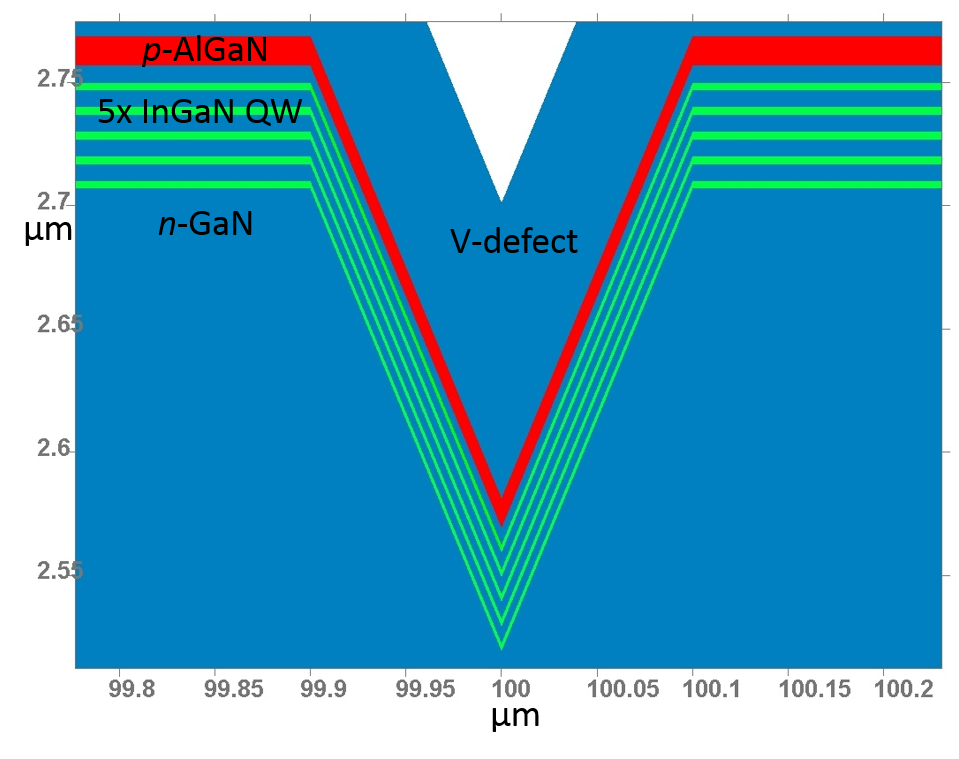
\includegraphics[width=0.6\textwidth]{Figs/Ch3/Sim}
	\caption[h] {Simulated LED structure.}
	\label{simsetup}
\end{figure}
\FloatBarrier 

The simulation results are shown in Fig.\ref{simresults}.. Fig.\ref{simresults}.a. shows overall radiative recombination events in units of $10^{28} cm^{-3}s^{-1}$. The region closest to the defect at the lowest QW shows an increased radiative recombination rate, indicating the presence of the defect can indeed cause enhanced radiative recombination under electrical injection in regions surrounding the defect, in agreement with the experimental observation of inhomogeneous EL. Fig.\ref{simresults}.b. shows two profiles taken from Fig.\ref{simresults}.a. intersecting the five QWs and indicates that the rate of radiative recombination is almost doubled in the lowest QW close to the defect when compared with a profile taken further away.\\
Under closer examination, Fig.\ref{simresults}.b. demonstrates that the 'bottom' QW dominates the overall emission, particularly close too the AlGaN inclusion. The carrier concentrations shown in Figures.\ref{simresults}a. and b show that this is primarily due to the enhanced hole concentration in the region adjacent to the AlGaN, as the electron concentration is relatively unchanged. Thus we can ascribe the enhanced local carrier concentration to the presence of the \textit{p}-AlGaN, which injects holes directly into the active region. The effects of hexagonal defect-assisted carrier injection into MQW stacks have been reported by Li \textit{et al.}, who reported that the disruption of the MQW stack by the hexagonal defect combined with thinner QBs allowed for the injection of holes up to 8 pairs of QWs away from the \textit{p}-GaN \cite{Li2014}. Quan \textit{et al.} have also suggested that hole injection via the semi-polar facets of the hexagonal defect occurs at a higher rate resulting in high radiative recombination near the defect, but larger defects may result in localised emission \cite{Quan2014}.

\begin{figure}[h]
	\begin{subfigure}[b]{0.45\textwidth}
		\centering
		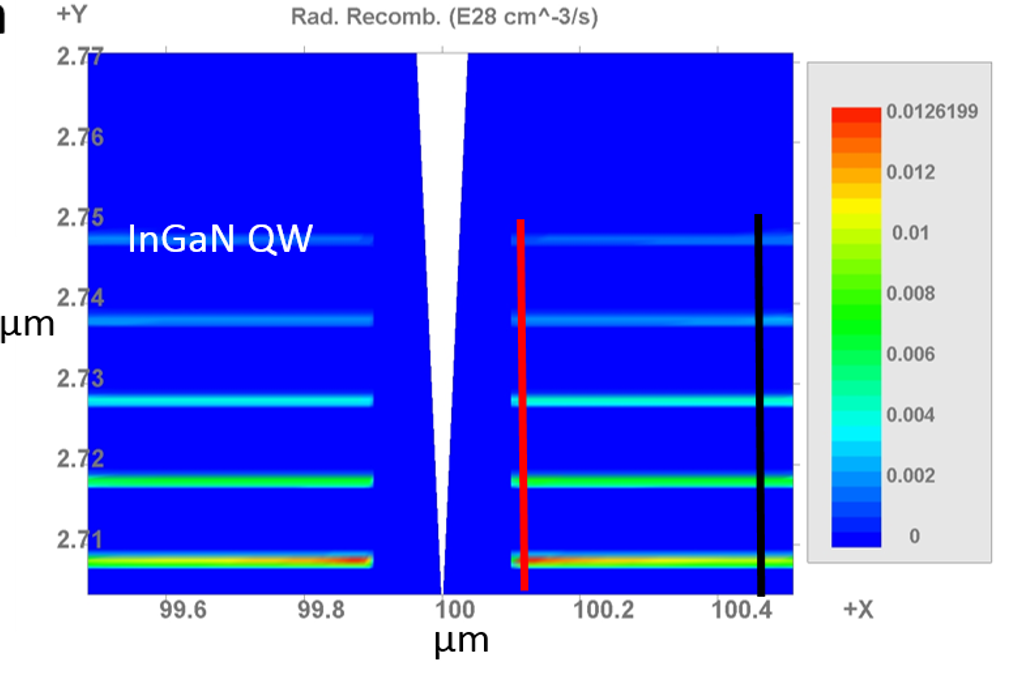
\includegraphics[width=1\linewidth]{Figs/Ch3/deep}
		\caption{}
	\end{subfigure}%
	\hspace*\fill
	\begin{subfigure}[b]{0.49\textwidth}
		\centering
		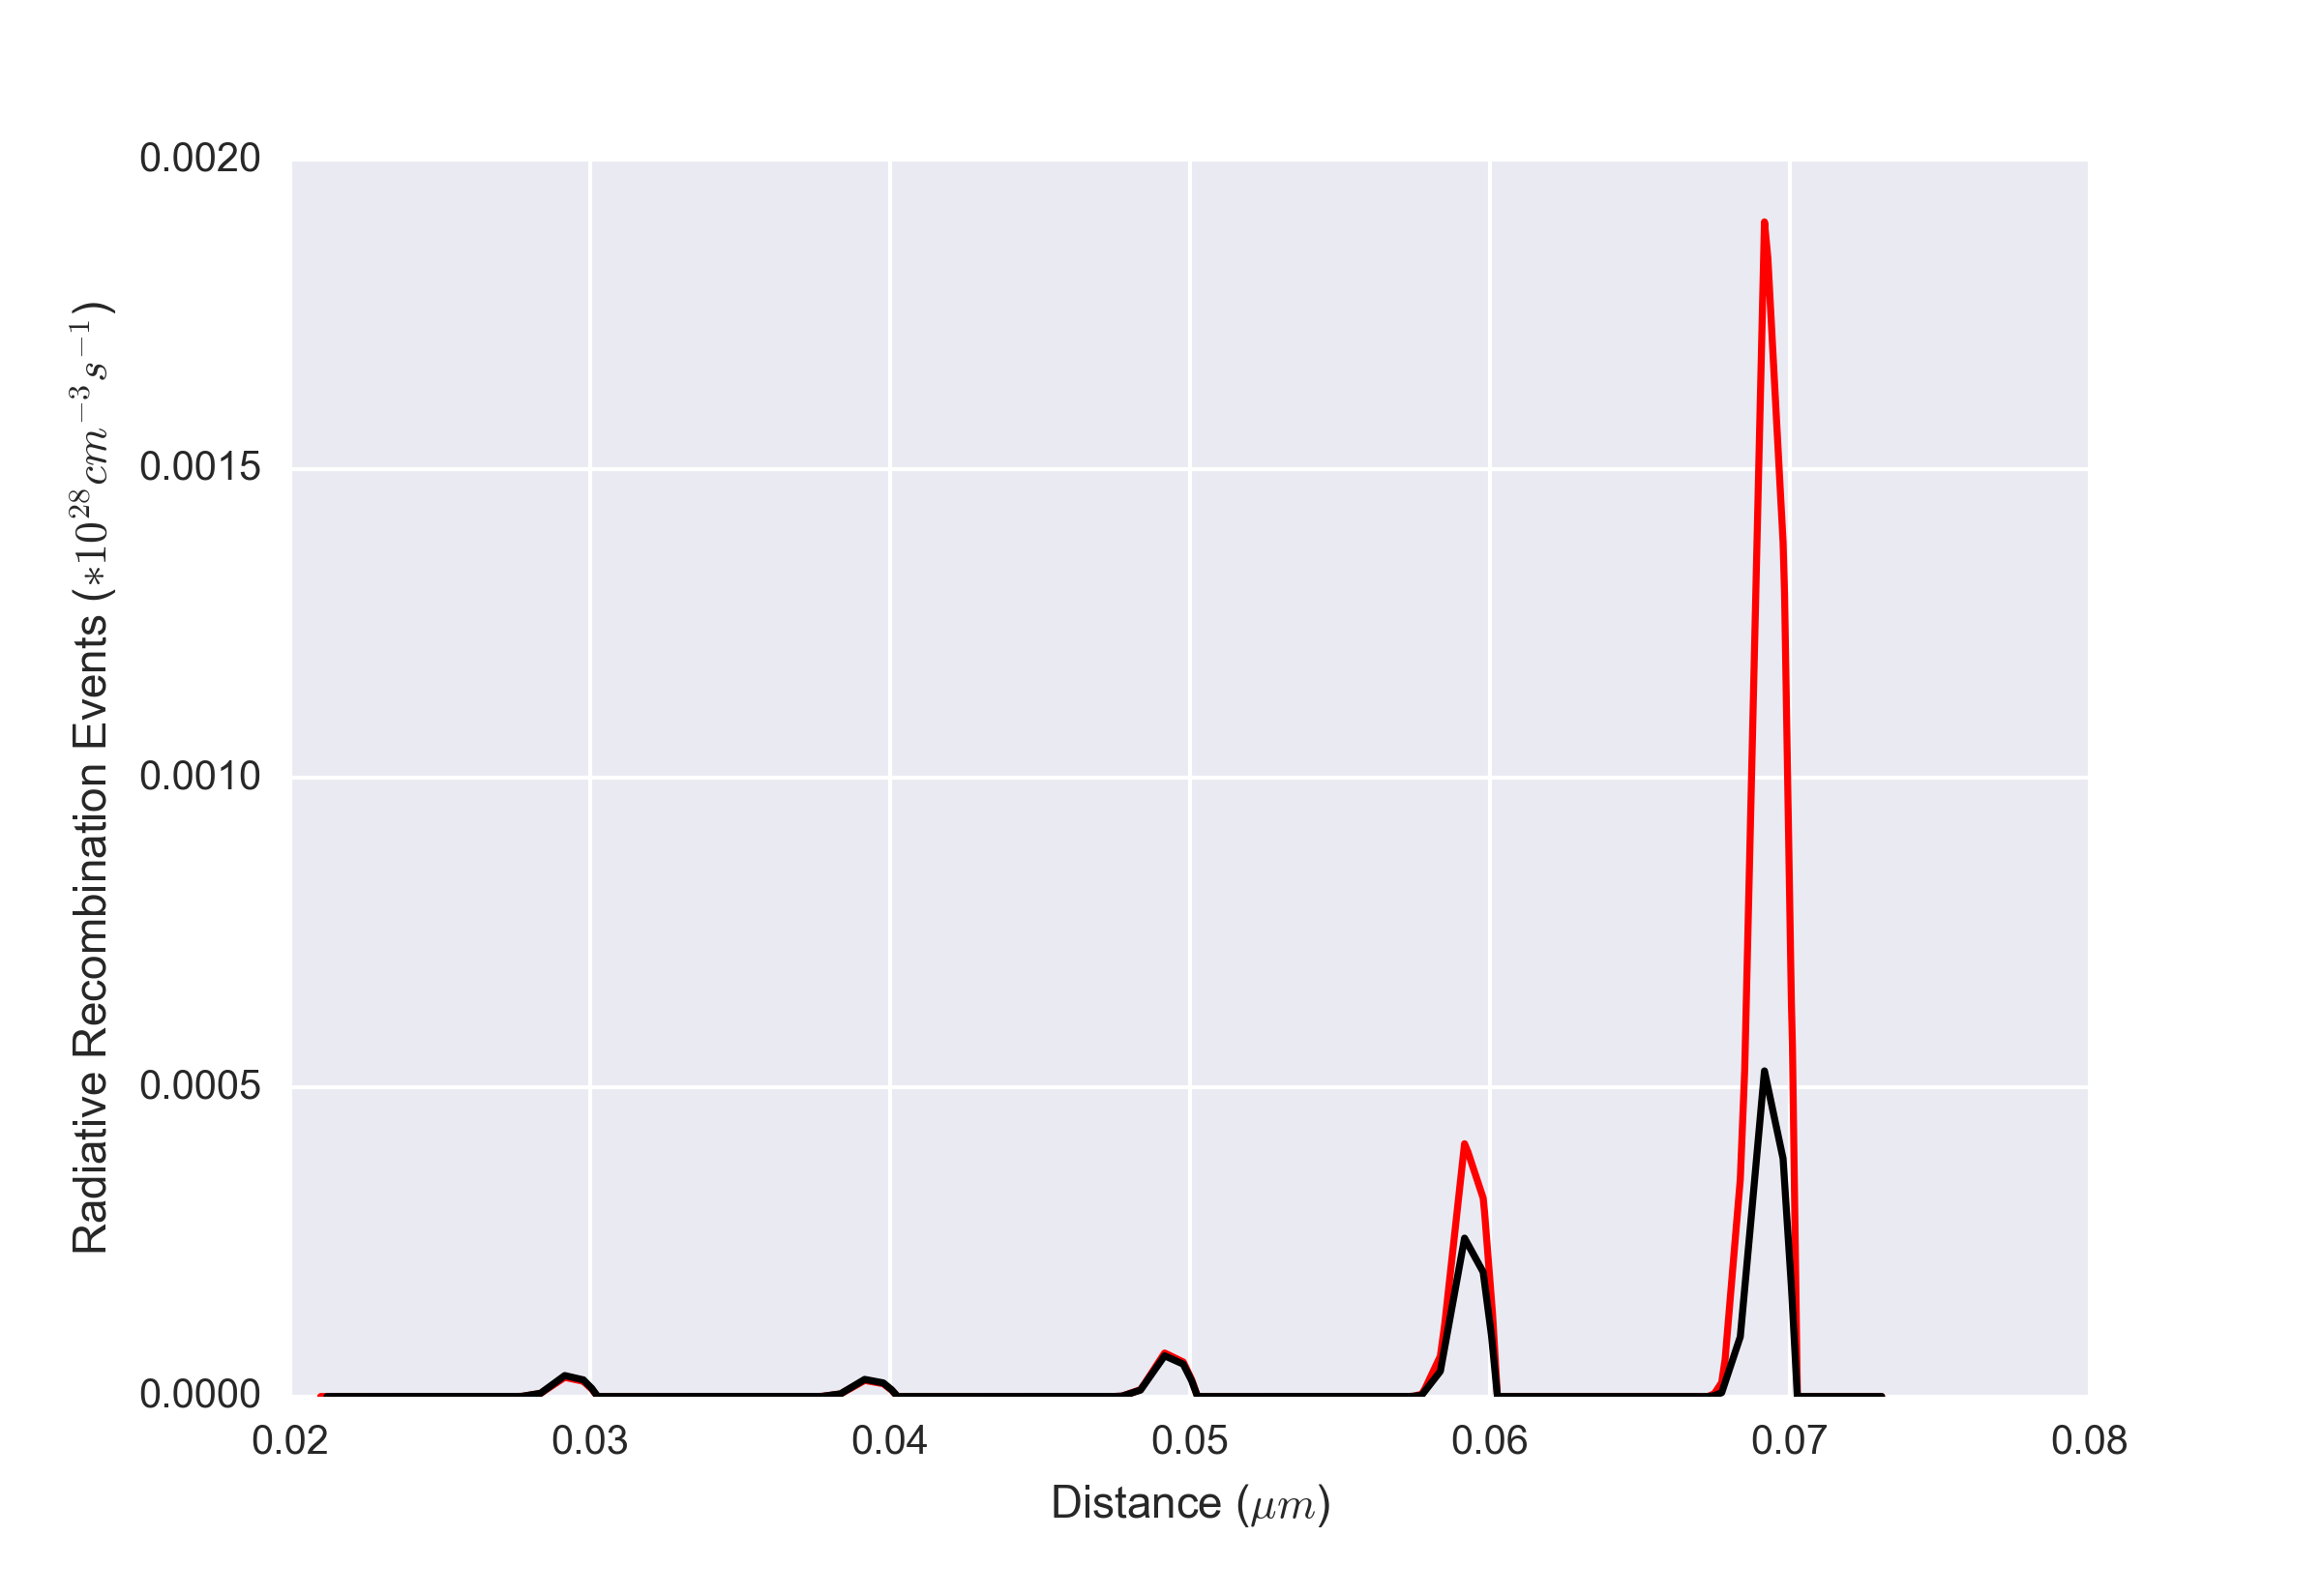
\includegraphics[width=1\linewidth]{Figs/Ch3/150rad}
		\caption{}		
	\end{subfigure}%
	
	\medskip
	\begin{subfigure}[b]{0.49\textwidth}
		\centering
		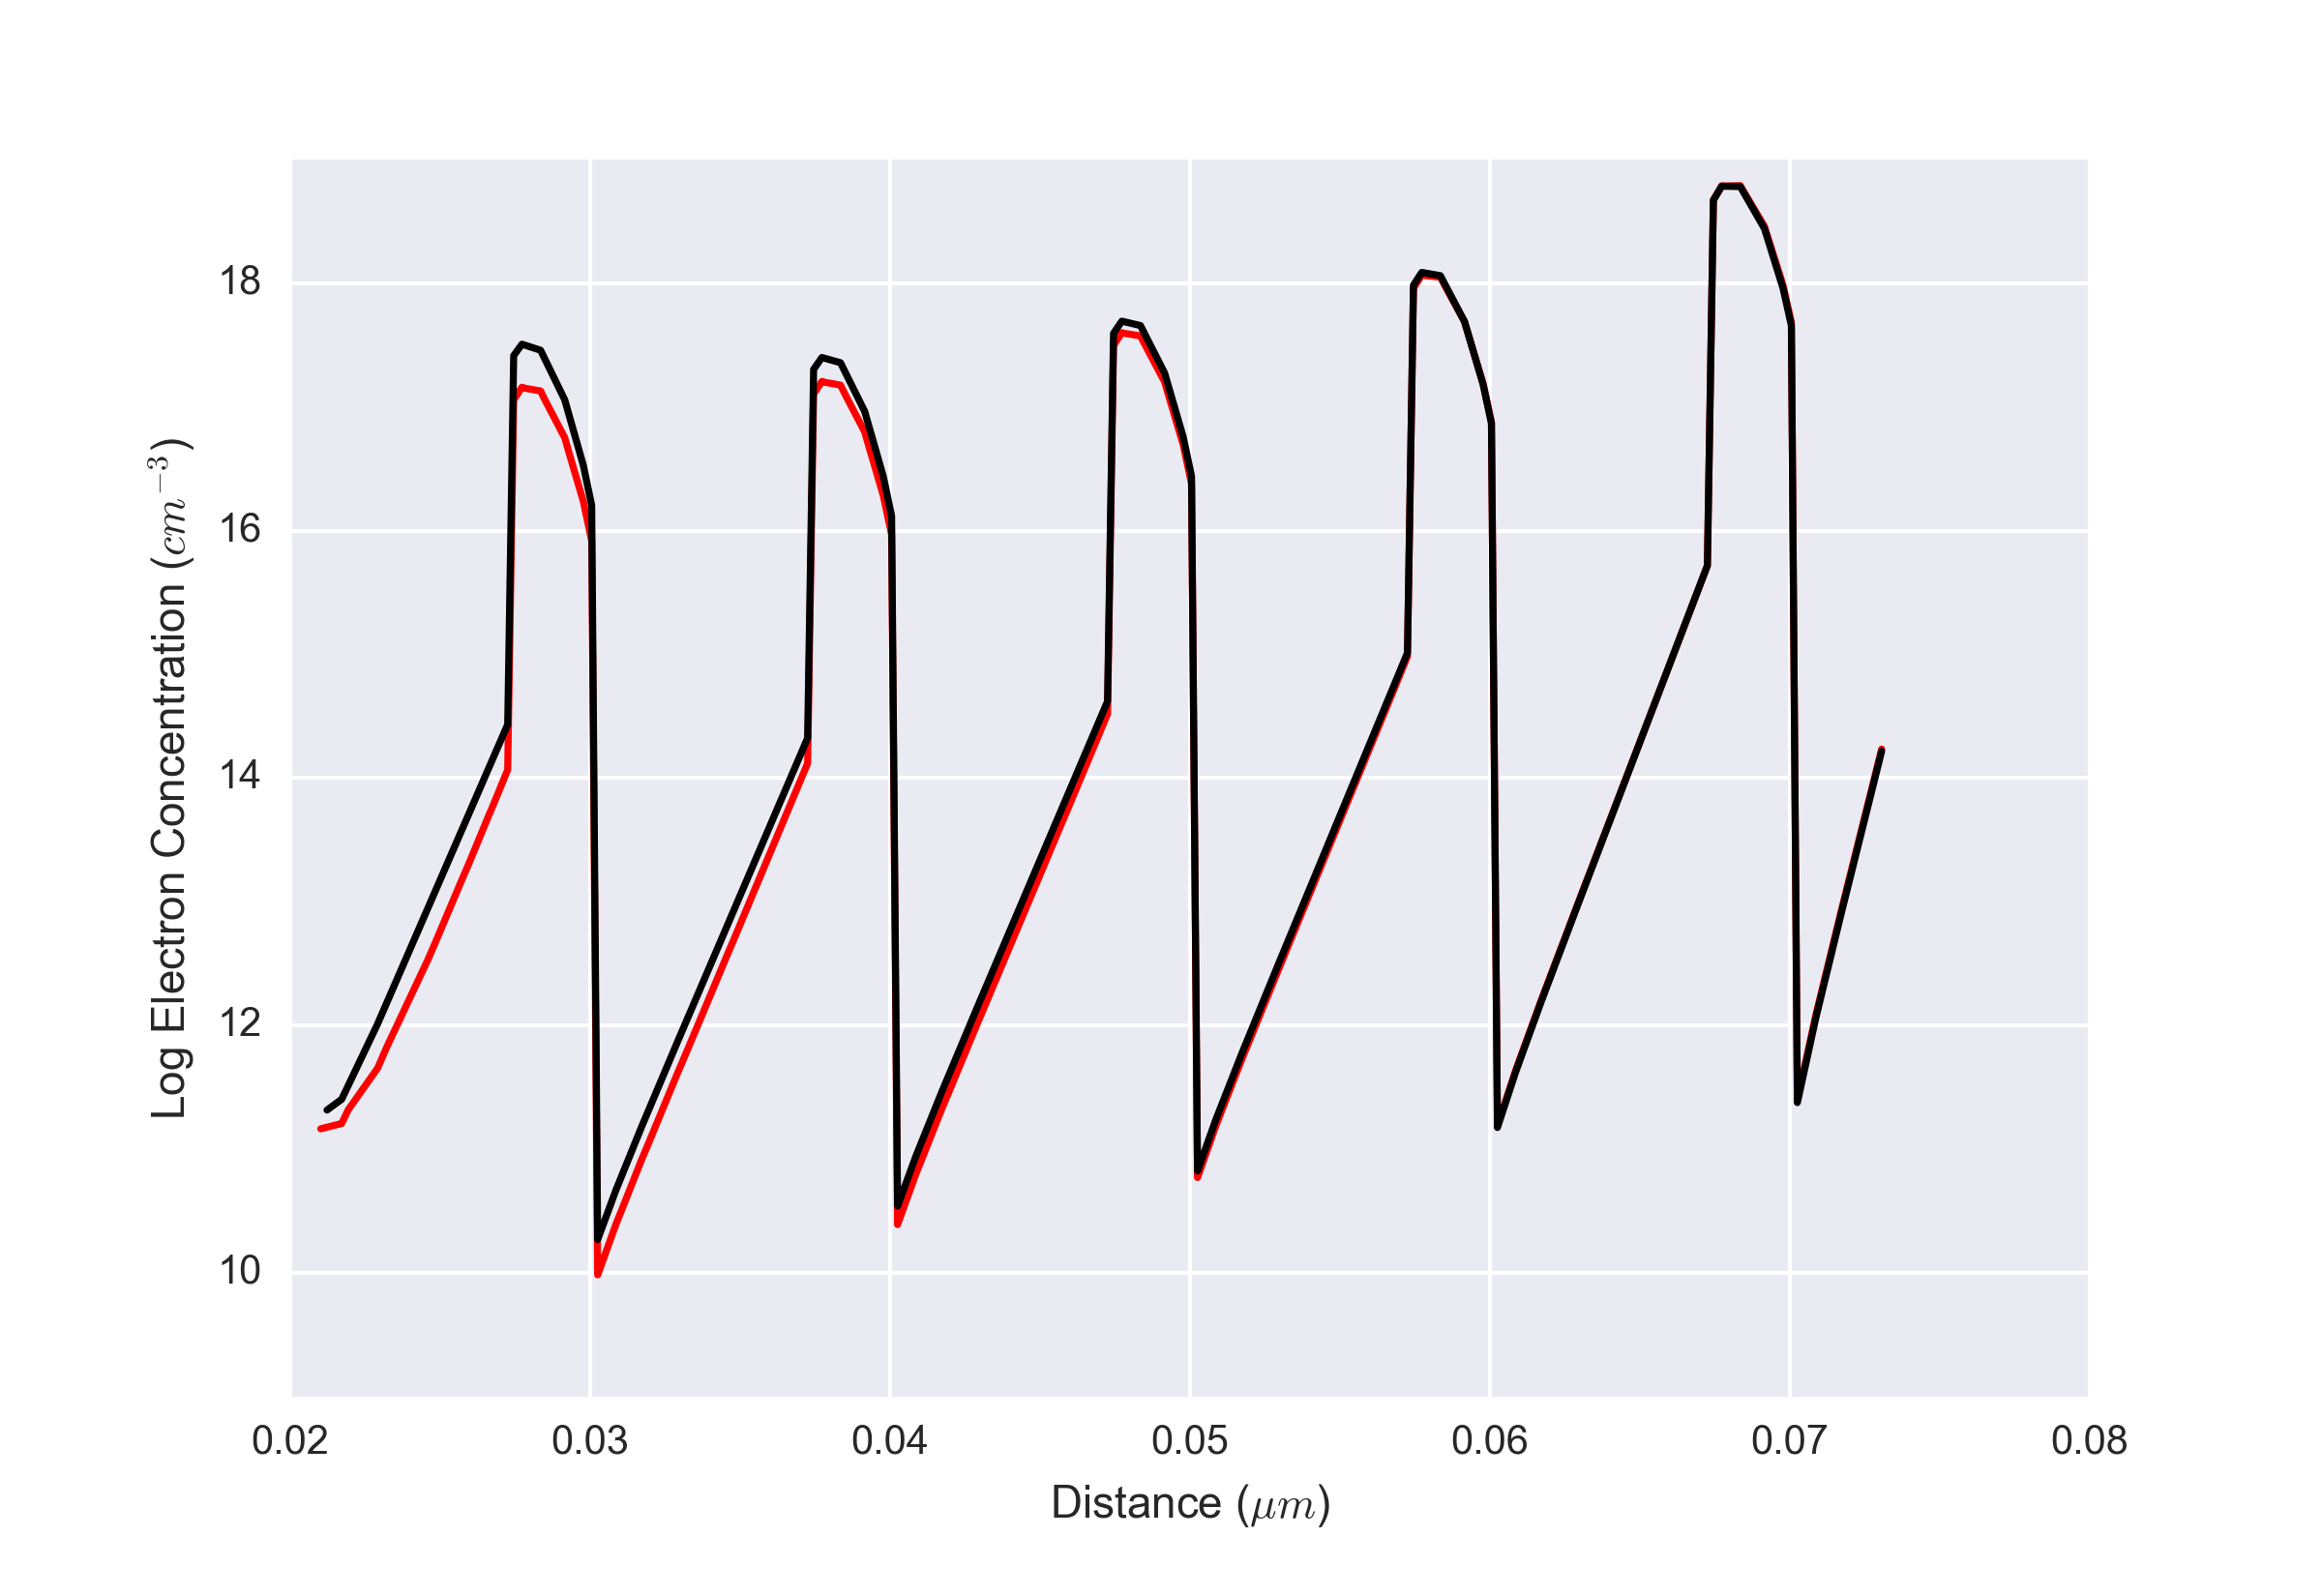
\includegraphics[width=1\linewidth]{Figs/Ch3/150elec}
		\caption{}
	\end{subfigure}%
	\hspace*\fill
	\begin{subfigure}[b]{0.49\textwidth}
		\centering
		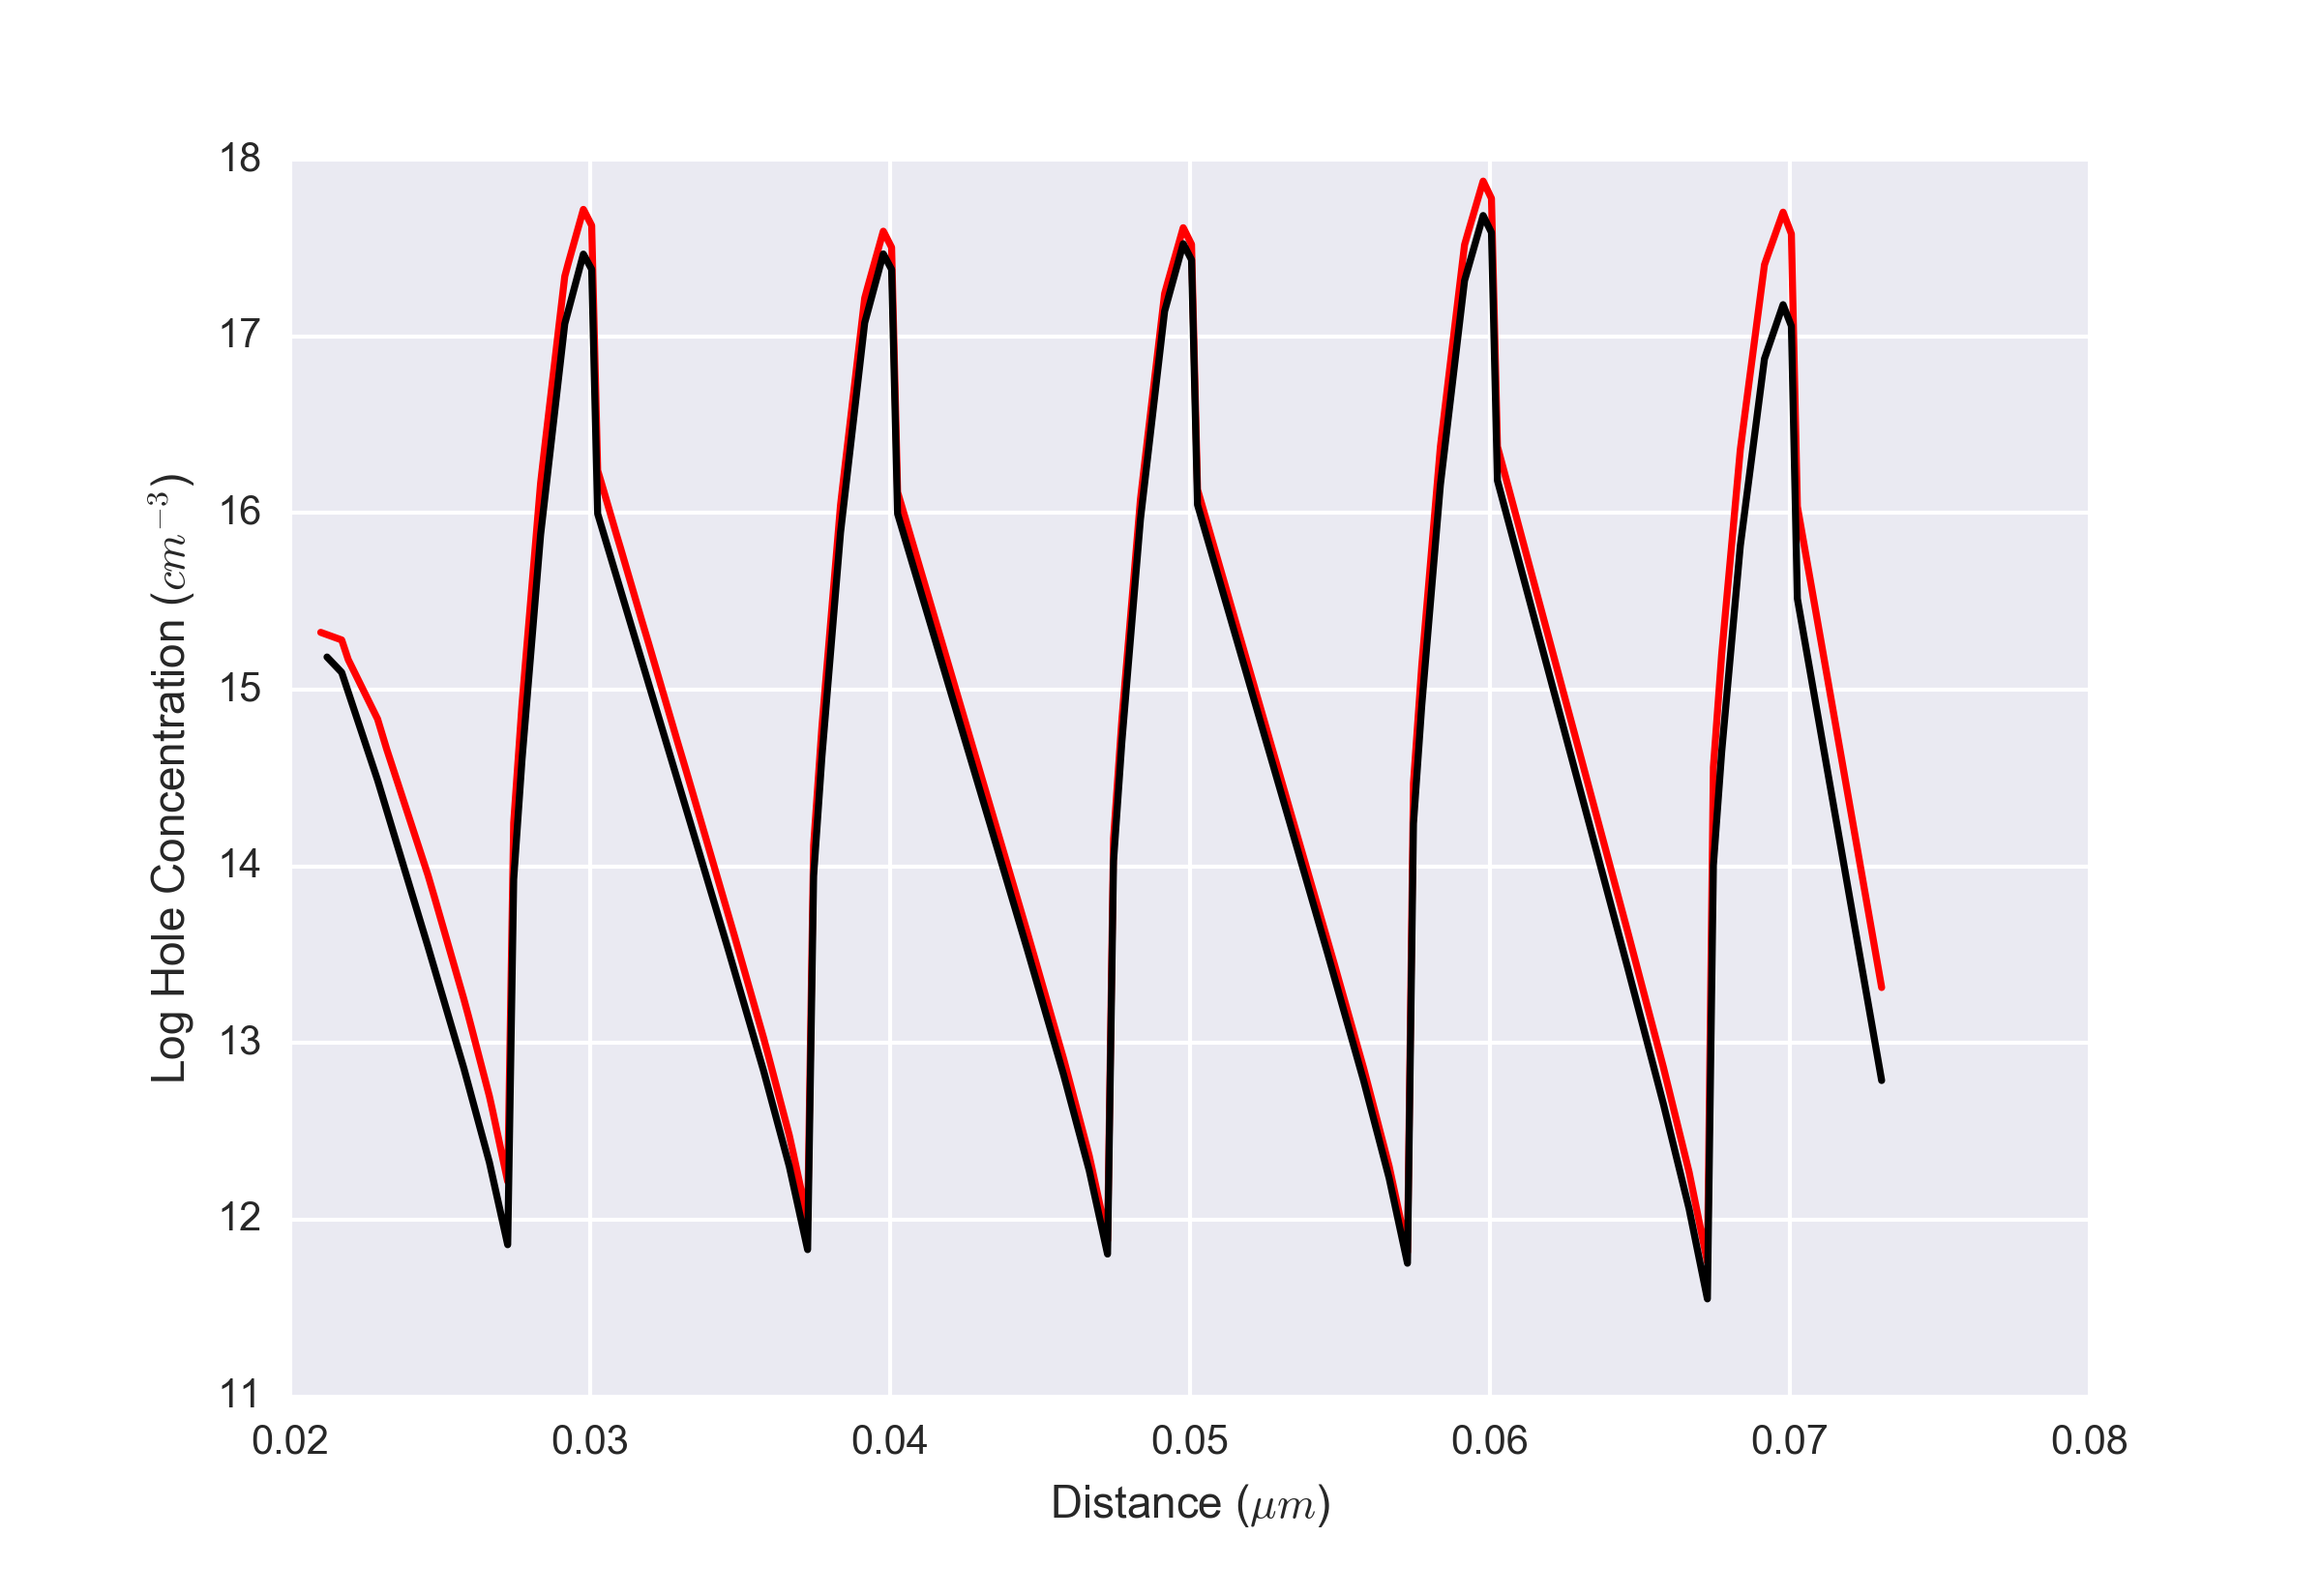
\includegraphics[width=1\linewidth]{Figs/Ch3/150hole}
		\caption{}		
	\end{subfigure}%
	
	
	\caption{APSYS simulation results: a) Radiative recombination events b) radiative recombination profiles, c) electron concentration profiles and d) hole concentration profiles. Red and black traces in b), c) and d) correspond to the red and black profiles in a).}
	\label{simresults}
\end{figure}
\FloatBarrier 

\subsubsection{Shallow Inclusion}

In this simulation we have simulated a structure similar to the composition maps shown in Fig.\ref{EDXspot}. We have assumed that the AlGaN EBL may penetrate only slightly in into the QW stack due to the defect, but otherwise the rest of the disrupted region is filled with undoped GaN. The AlGaN EBL doping is set to 5$\times 10^{18} cm^{-3}$ with an Al content of 10$\%$. Thus, in this case we assume no projection artifacts, as opposed to the deep Al inclusion simulated previously. The geometry used for this simulation is shown in Fig.\ref{shallowgeom}.

\begin{figure}[h]
	\centering
	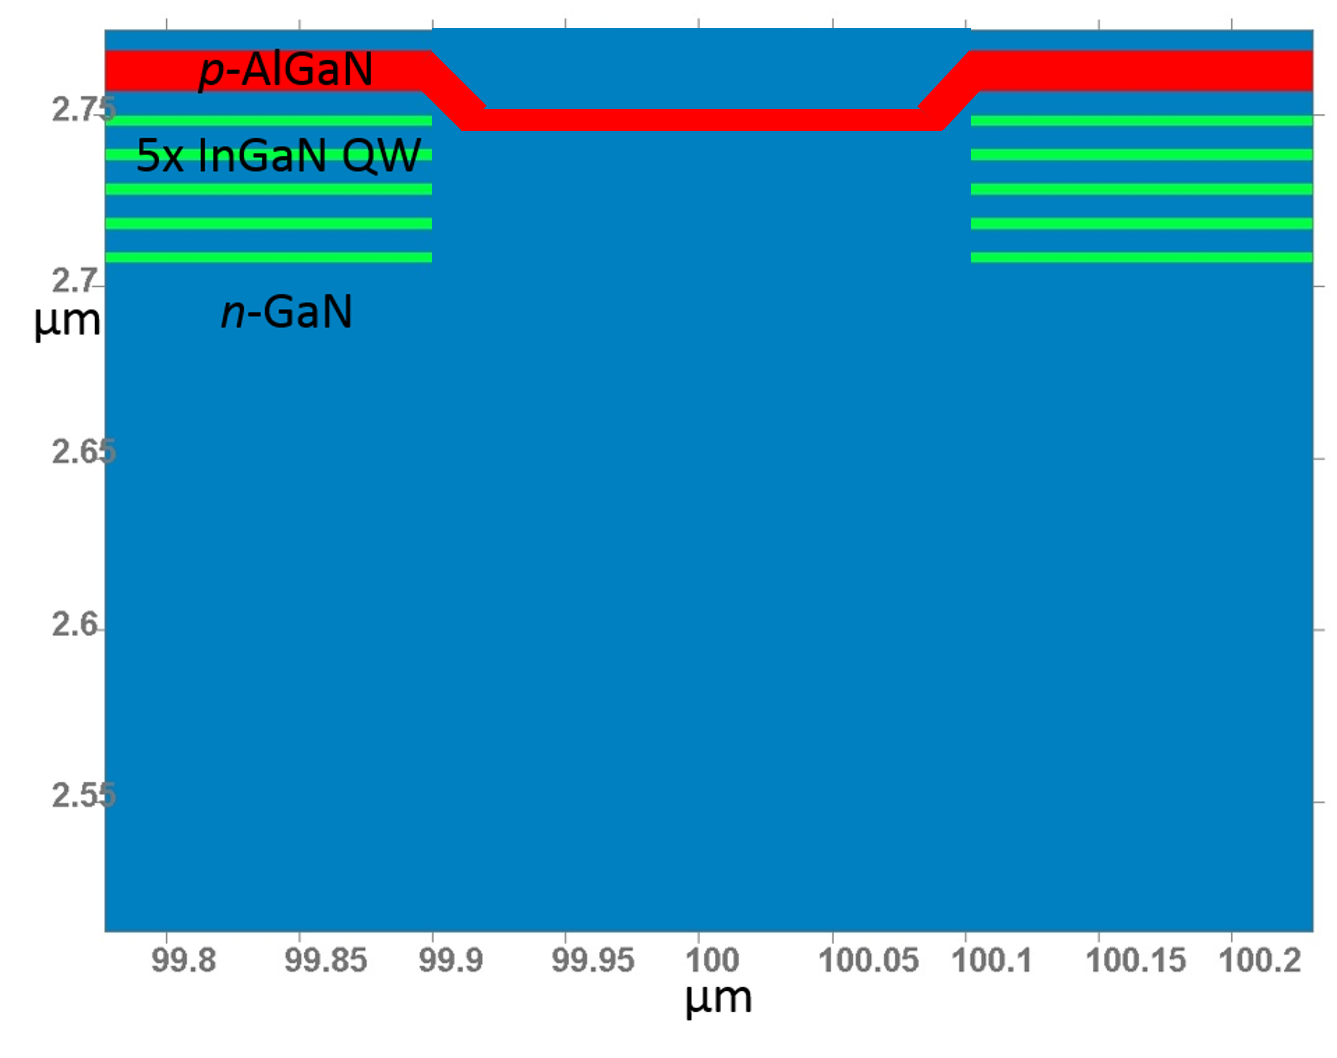
\includegraphics[width=0.6\textwidth]{Figs/Ch3/shallow}
	\caption[h] {Simulated LED structure for the shallow inclusion.}
	\label{shallowgeom}
\end{figure}
\FloatBarrier 

Fig.\ref{shallowres} shows the simulation results. Fig.\ref{shallowres}.a. shows that radiative recombination is enhanced in the vicinity of the shallow inclusion, particularly in the second QW (QW2) from the EBL due to carrier injection from the semi-polar facets of the defect. Fig.\ref{shallowres}.c. and Fig.\ref{shallowres}.d. show that the hole concentration is responsible for the local enhancement in radiative recombination near the shallow inclusion as the electron concentration is mostly unchanged. Fig.\ref{shallowres} show that the enhanced injection of holes results in an order of magnitude increase in radiative recombination in QW2. As such, even in the case of a 'shallow' \textit{p}-AlGaN inclusion induced by a hexagonal defect, the injection of holes into the active region still results in enhanced emission adjacent to the defect.

\begin{figure}[h]
	\begin{subfigure}[b]{0.45\textwidth}
		\centering
		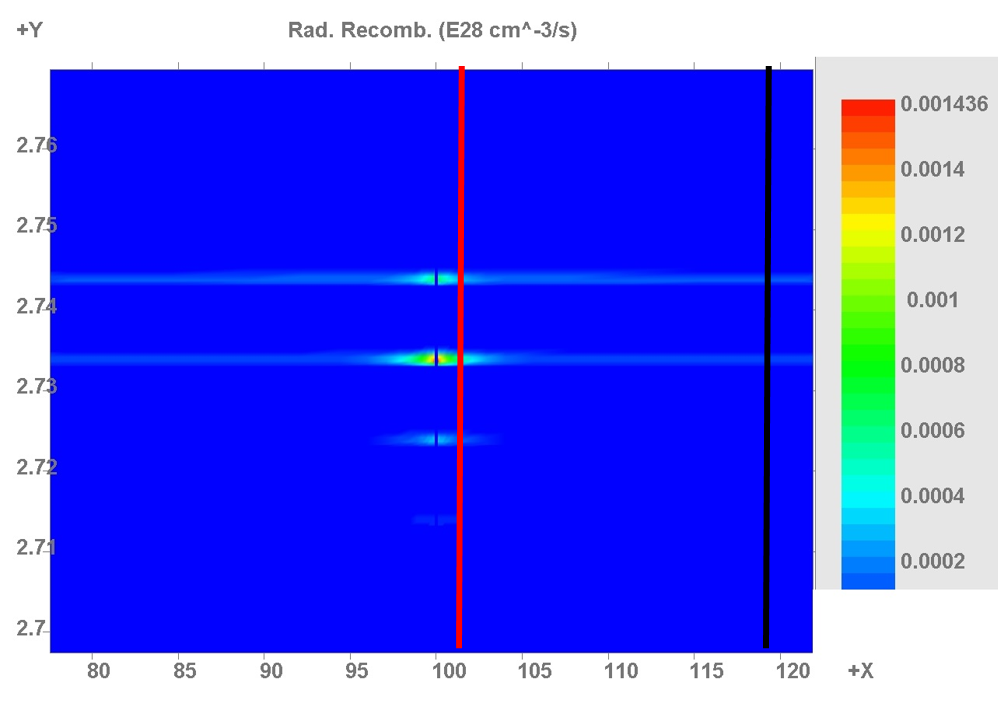
\includegraphics[width=1\linewidth]{Figs/Ch3/shallowrad1}
		\caption{}
	\end{subfigure}%
	\hspace*\fill
	\begin{subfigure}[b]{0.49\textwidth}
		\centering
		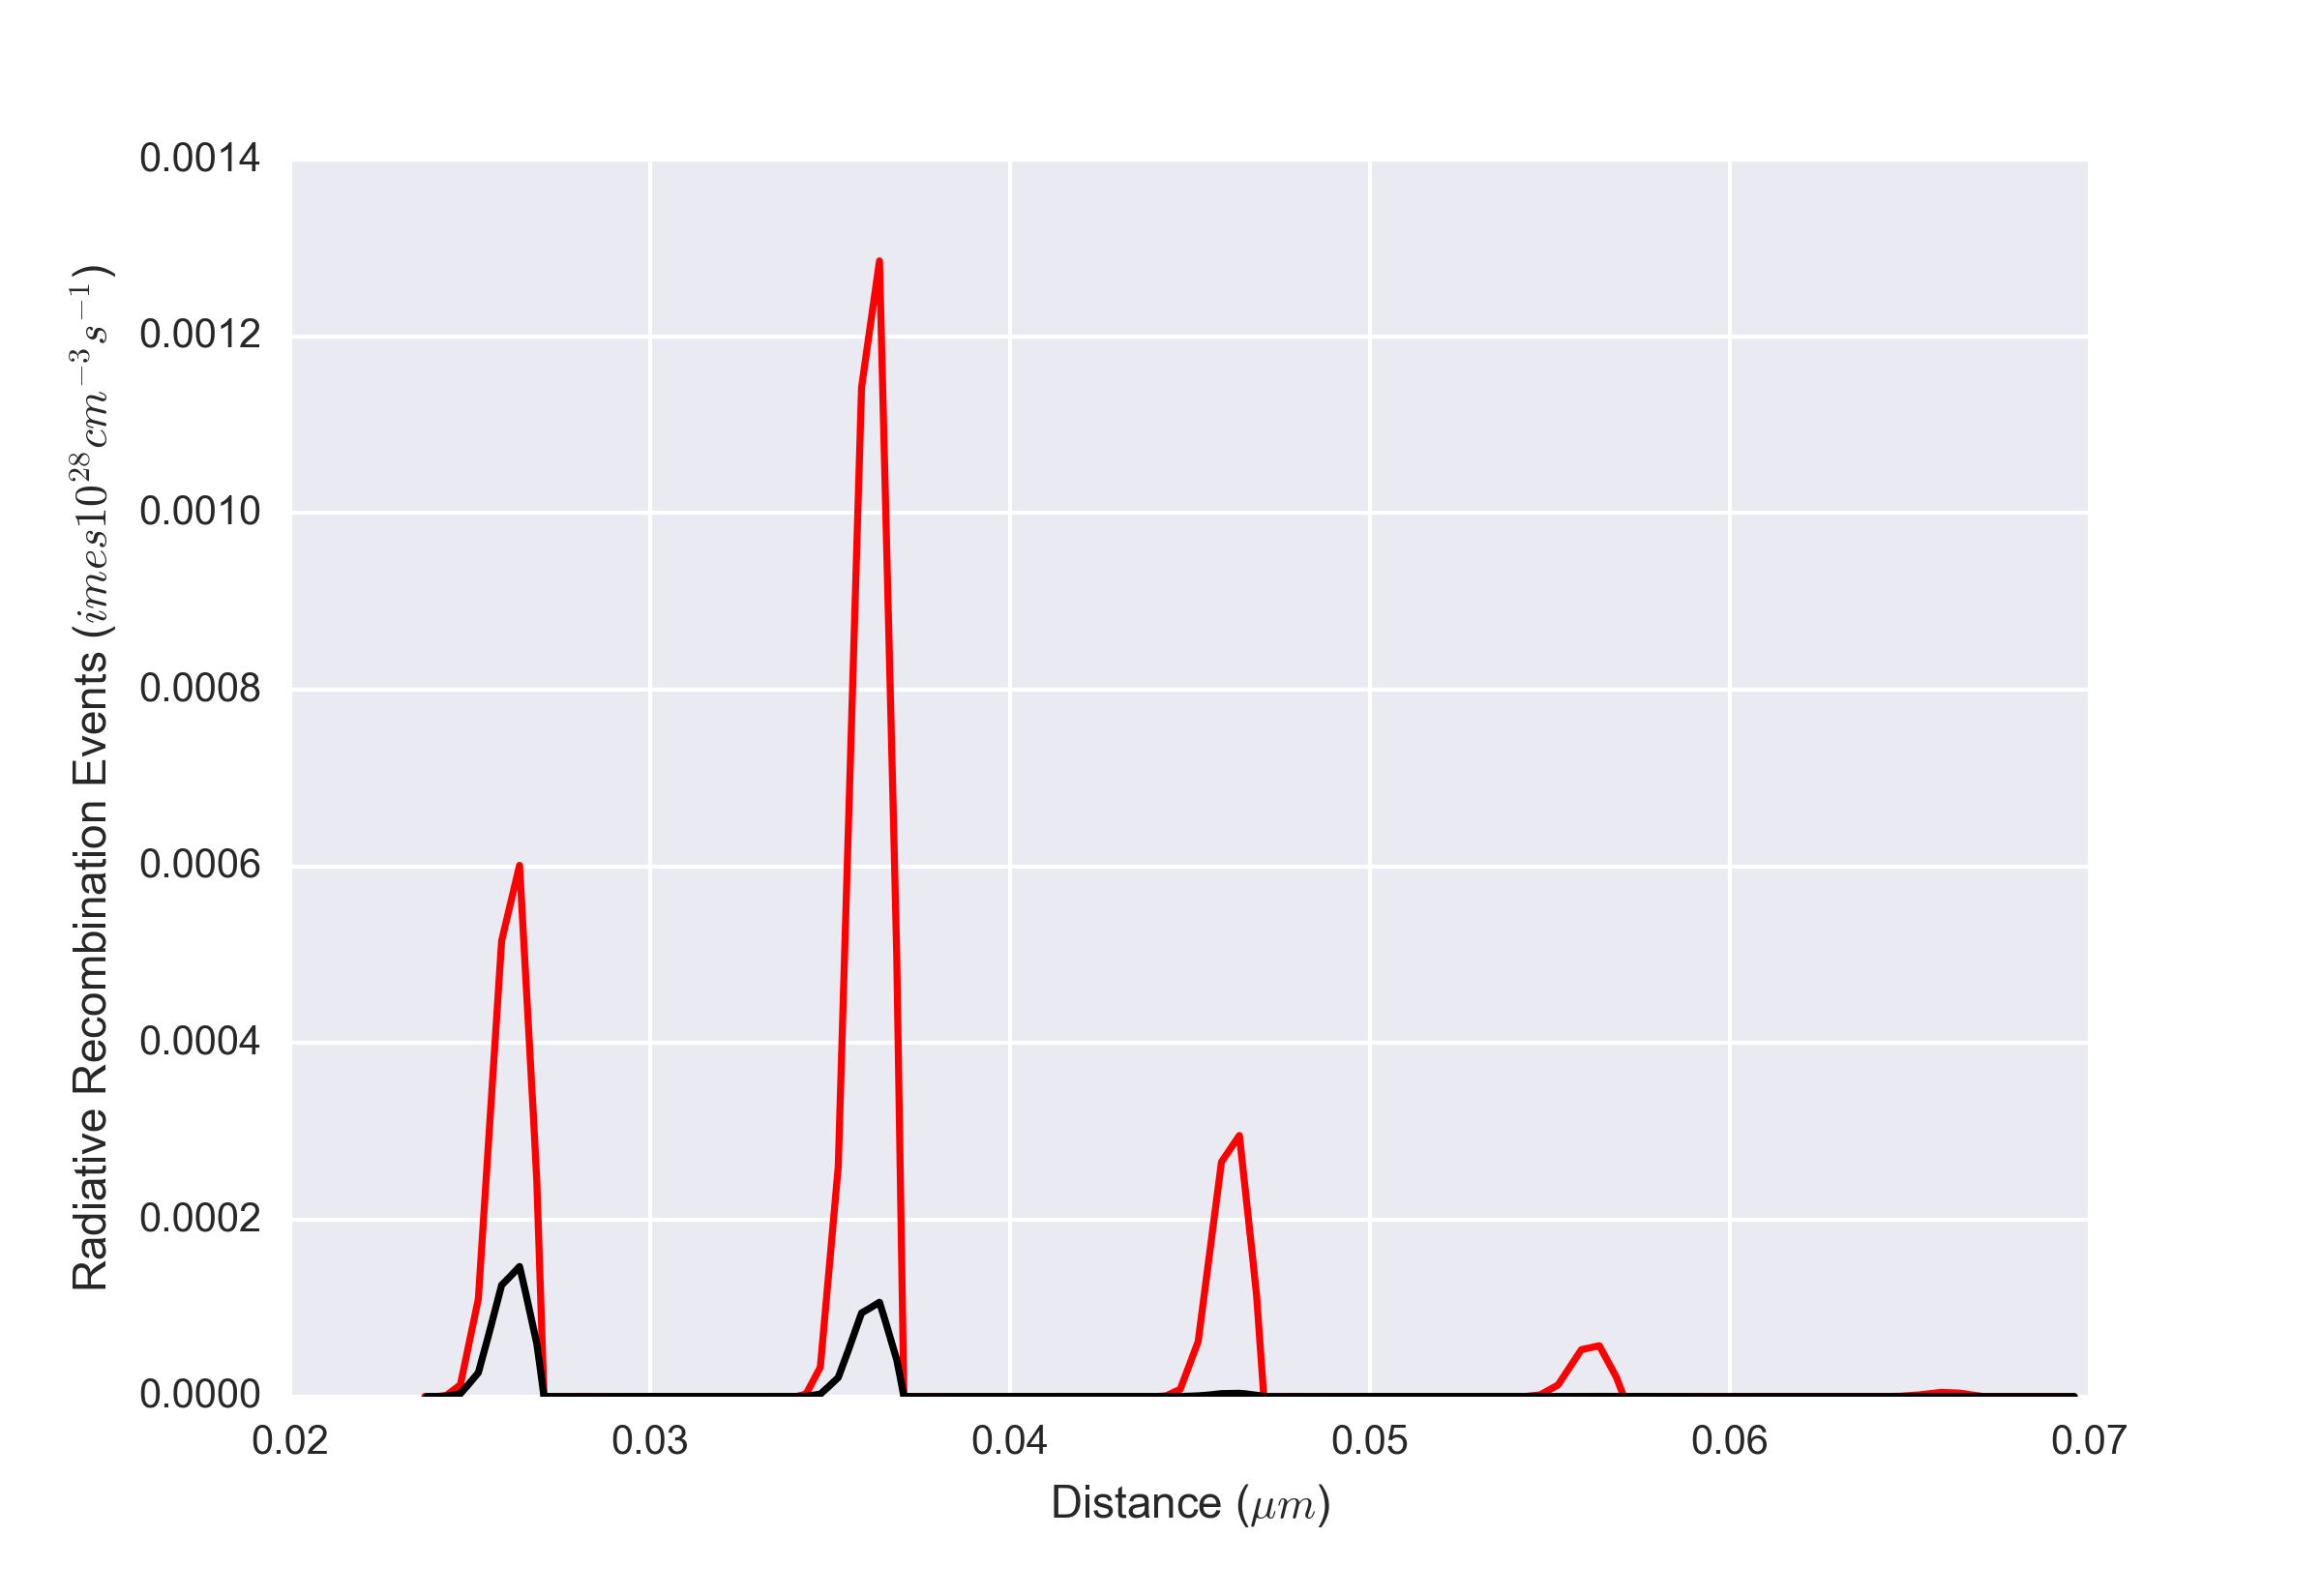
\includegraphics[width=1\linewidth]{Figs/Ch3/shallowrad}
		\caption{}		
	\end{subfigure}%
	
	\medskip
	\begin{subfigure}[b]{0.49\textwidth}
		\centering
		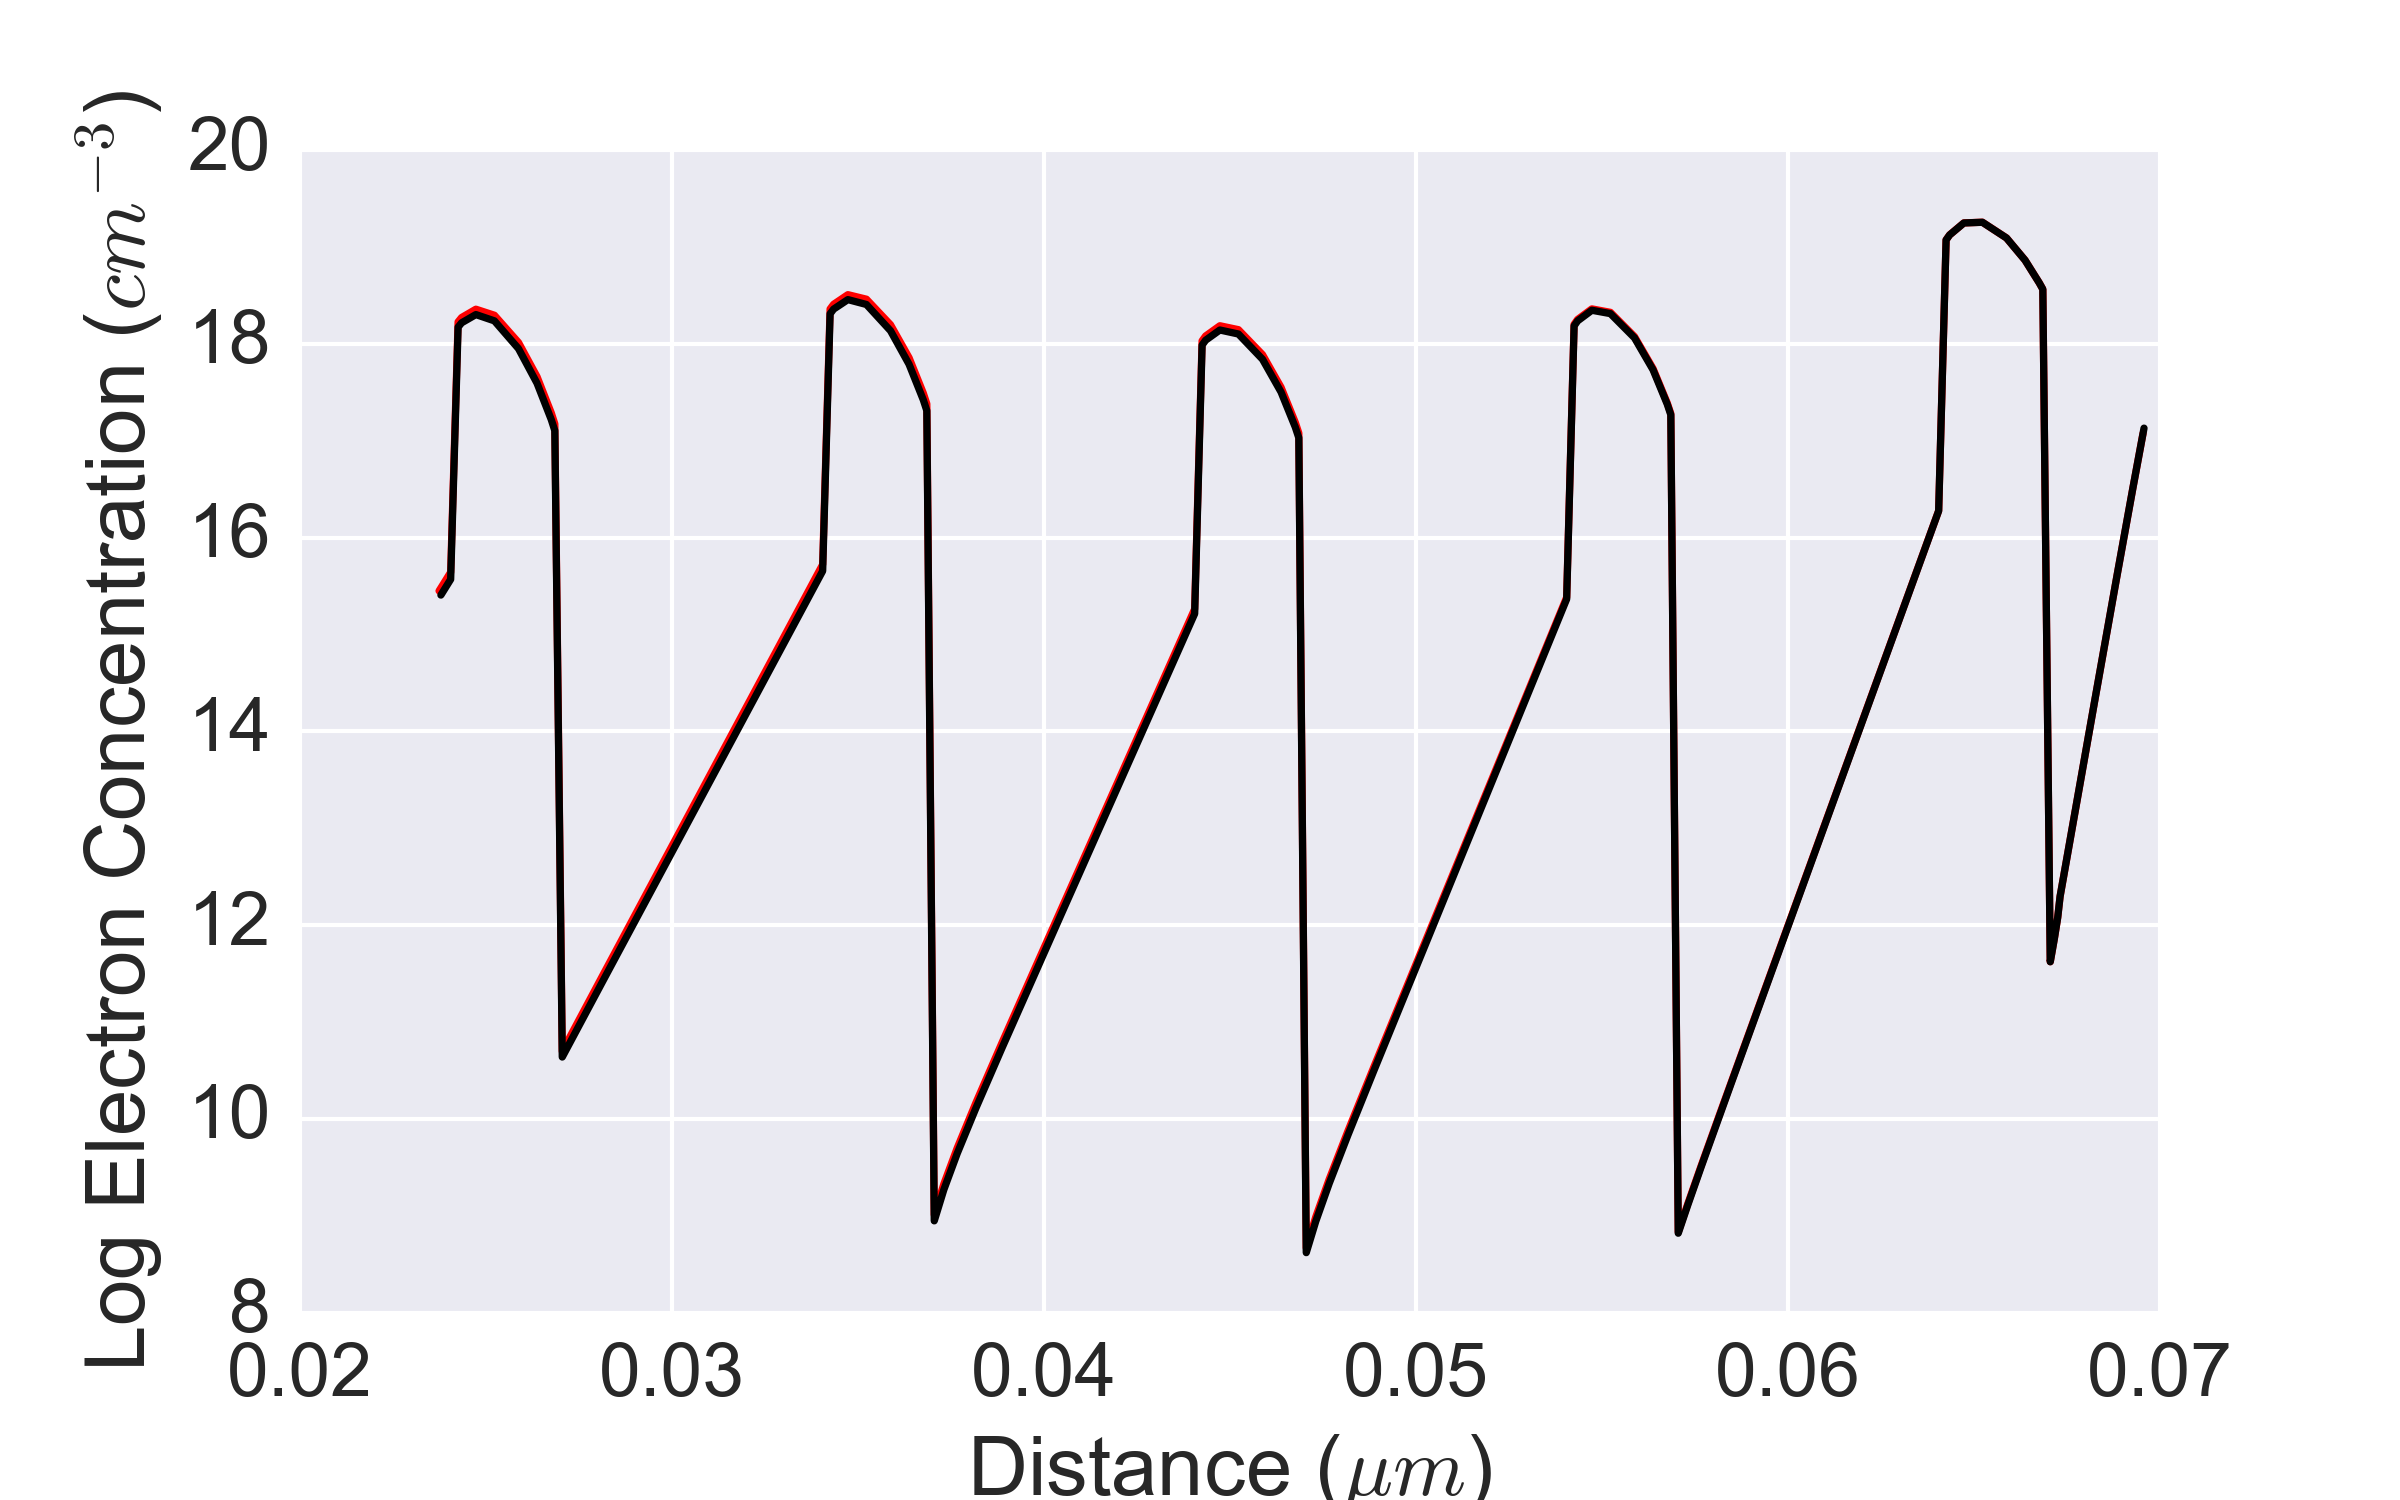
\includegraphics[width=1\linewidth]{Figs/Ch3/shallowelec}
		\caption{}
	\end{subfigure}%
	\hspace*\fill
	\begin{subfigure}[b]{0.49\textwidth}
		\centering
		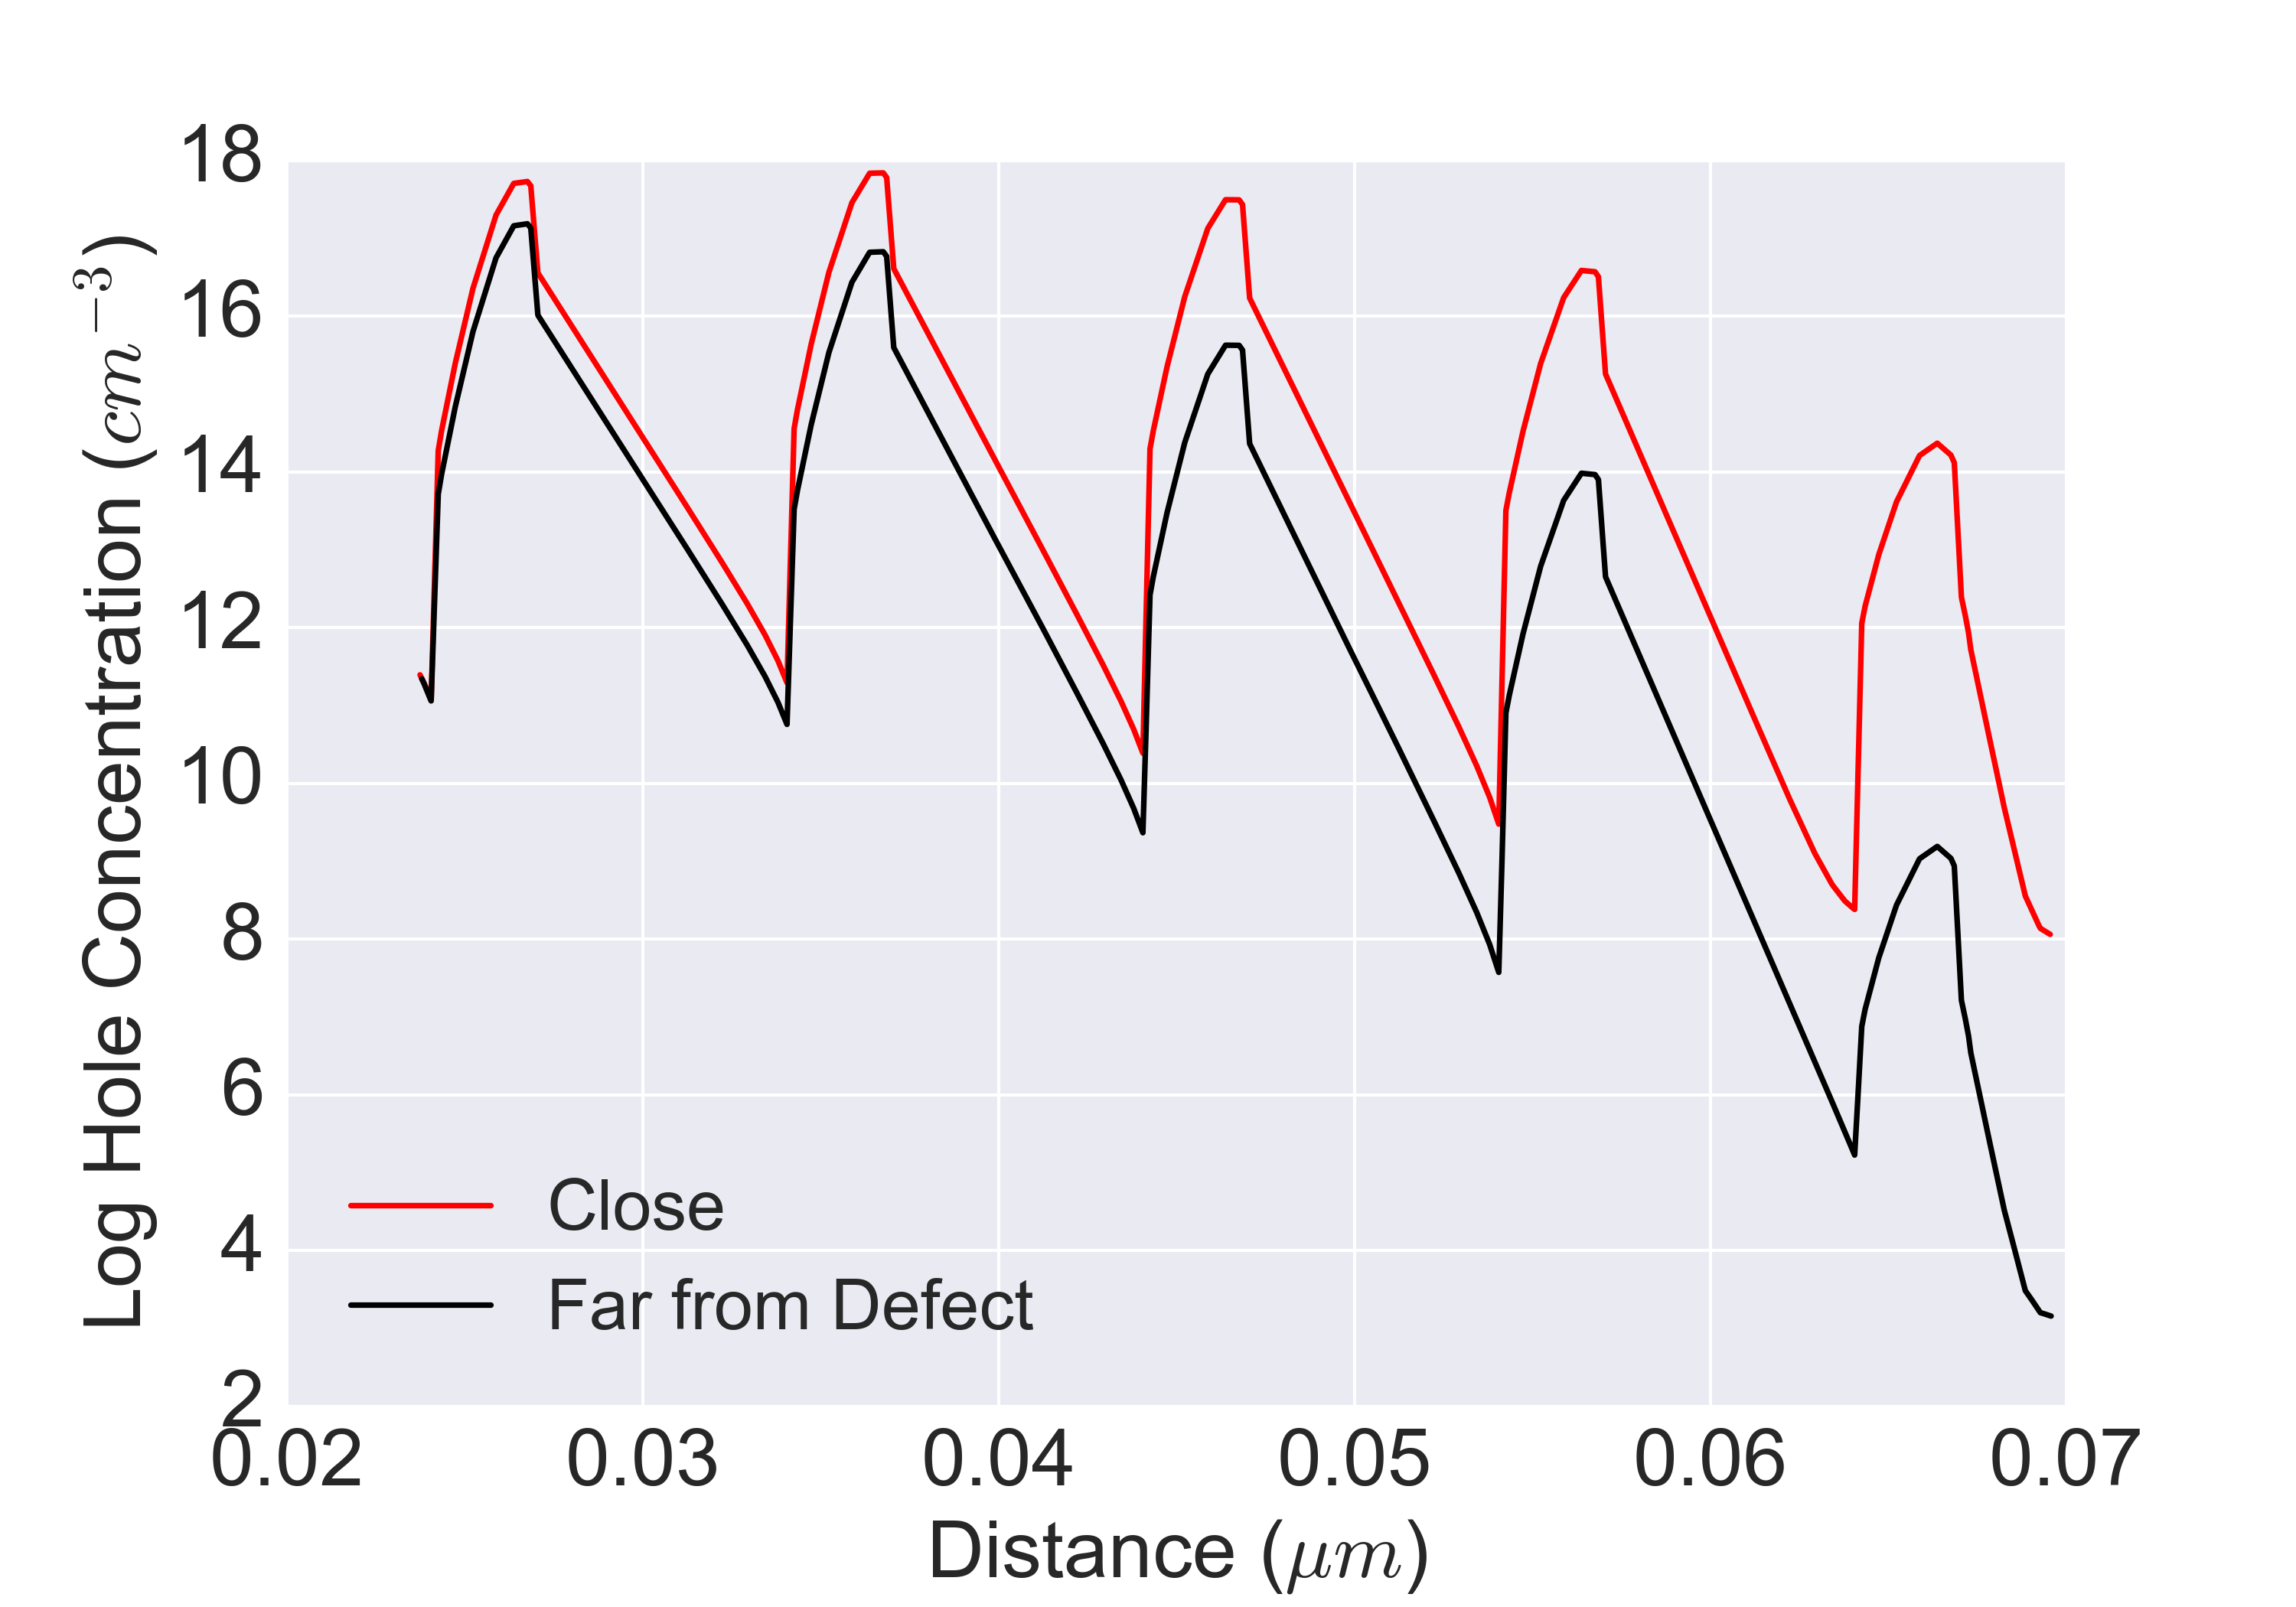
\includegraphics[width=1\linewidth]{Figs/Ch3/shallowhole}
		\caption{}		
	\end{subfigure}%
	
	
	\caption{APSYS simulation results: a) Radiative recombination events b) radiative recombination profiles, c) electron concentration profiles and d) hole concentration profiles. Red and black traces in b), c) and d) correspond to the red and black profiles in a).}
	\label{shallowres}
\end{figure}
\FloatBarrier 

\subsection{Origin of the Defect}
In the previous sections we have established the cause of the inhomogeneous EL to be the presence of large hexagonal defects. However, it is also important to establish the origin of these hexagonal defects, as their elimination is the key to the production of LEDs with uniform emission, unlike those studied here.

\subsubsection{Threading Dislocation Analysis}

Hexagonal defects are typically associated with threading dislocations \cite{Florescu2003}, as such we performed TEM on the FIB prepared lamella in order to observe threading dislocation associated with the hexagonal defects observed at the centre of inhomogeneities in the EL. The TEM image is shown in Fig. \ref{TEM-spot}. Interestingly, rather than a single TD, we can observe a 'bundle' of dislocations associated with the defect with several 'loops' also apparent.

\begin{figure}[h]
	\centering
	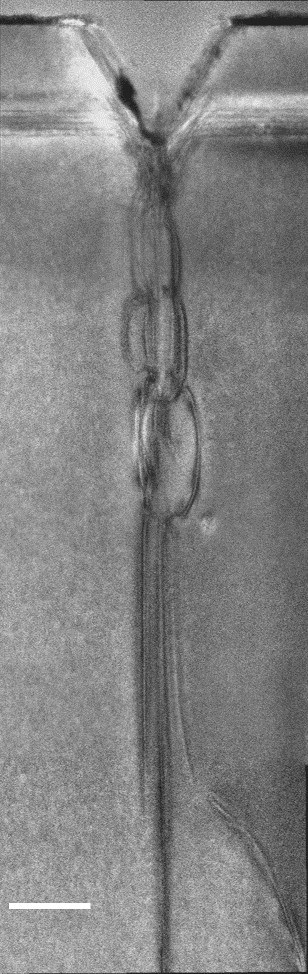
\includegraphics[width=0.4\textwidth]{Figs/Ch3/TEMspot}
	\caption[h] {TEM image viewed along the $(10\bar{1}0)$ direction of the dislocations associated with the hexagonal defect shown in Fig.\ref{STEM-spot}. The scale bar corresponds to a  length of 200 nm.}
	\label{TEM-spot}
\end{figure}
\FloatBarrier 

In order to characterise the dislocations shown in Fig.\ref{TEM-spot}, WBDF-TEM was performed. The results are shown in Fig.\ref{WBDF-spot}.
\begin{figure}[h]
	\centering
	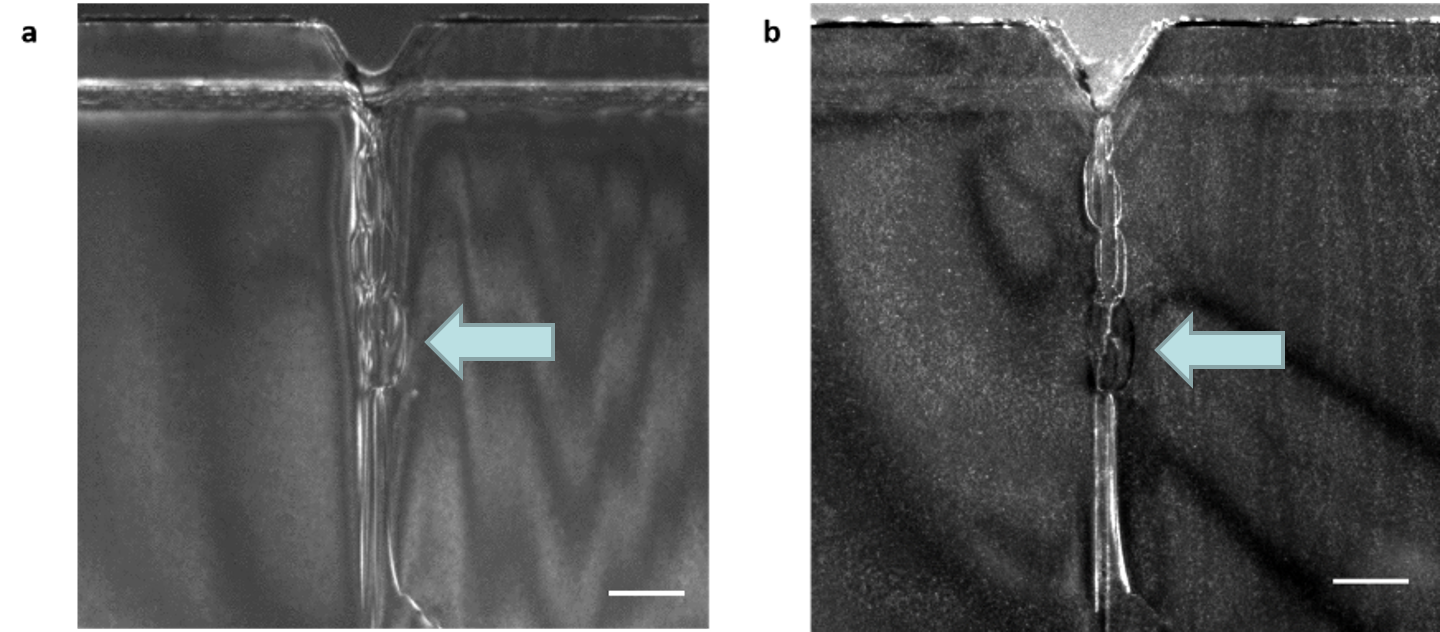
\includegraphics[width=1\textwidth]{Figs/Ch3/WBDF-yall}
	\caption[h] {WBDF-TEM of TDs associated with the hexagonal defect under a) \textbf{g}=$<11\bar{2}0>$ and b) \textbf{g}=$<0001>$. The scale bar corresponds to a length of 150 nm.}
	\label{WBDF-spot}
\end{figure}
\FloatBarrier 

Fig.\ref{WBDF-spot} shows that the majority of TDs associated with the pit are mixed in nature, with some exceptions such as the 'dislocation loop' which shows no contrast under when viewed under the condition \textbf{g}=$<0001>$. Nonetheless, the number of TDs associated with a single defect here is astonishing.\\
The bundle of TDs observed here could potentially be attributed to the vertical side facets in GaN islands during the inital growth of the GaN template on sapphire. Datta \textit{et al.} showed that threading dislocations associated with basal plane stacking faults are located at coalescence boundaries between two GaN grains, and can open up into hexagonal defects at the surface, as shown in Fig.\ref{Datta} \cite{Datta2004}. In order to avoid GaN grains with vertical side facets, Datta \textit{et al.} suggest initialising epilayer growth at a low V/III ratio or increased pressure as these conditions favour the formation of GaN islands with inclined side facets\cite{Hiramatsu2001,Beaumont1999}, thus allowing TDs to bend laterally during film coalescence rather than propagate upwards towards the epilayer surface and form hexagonal defects.

\begin{figure}[h]
	\centering
	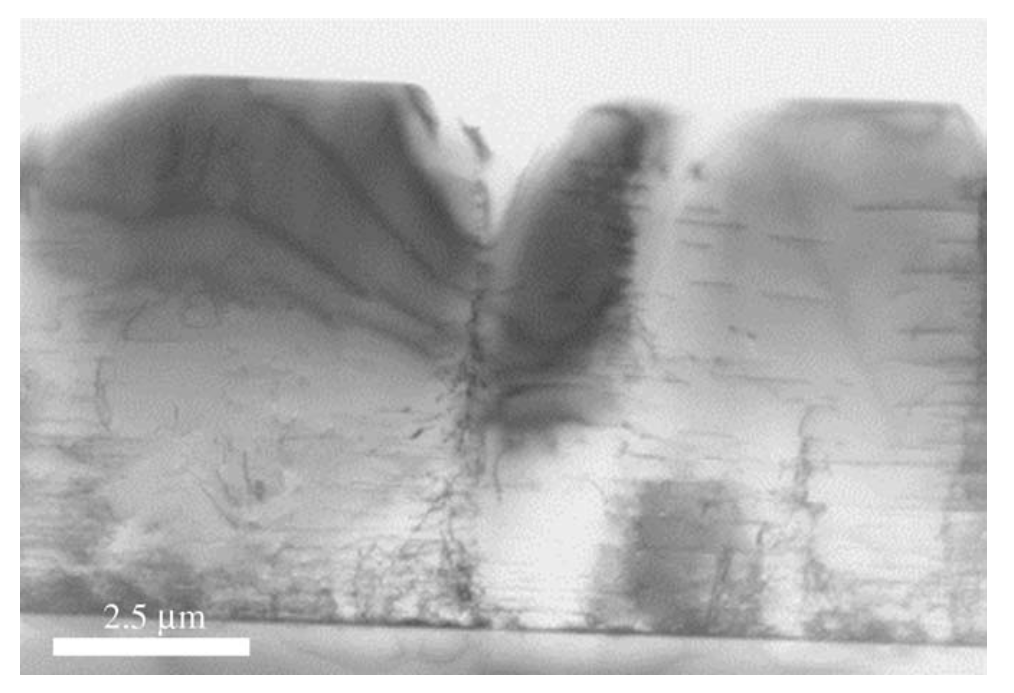
\includegraphics[width=1\textwidth]{Figs/Ch3/Datta}
	\caption[h] {BF-TEMimage of a coalescence boundary between two GaN grains and associated threading dislocations opening up into a hexagonal defect \cite{Datta2004}. }
	\label{Datta}
\end{figure}
\FloatBarrier 


\section{Conclusion}

First and foremost we have utilised a host of microscopy techniques to identify the cause of inhomogeneous EL in III-nitride LEDs. Hyperspectral EL mapping was performed over a set of inhomogeneities in order to determine their spectral properties. Using this data, the inhomogeneities were established to be blueshifted and have a larger emission FWHM. Further current dependent EL-measurements revealed that the inhomogeneities exhibited emissive properties consistent with higher local carrier concentration.\\
SEM-based techniques were used to further elucidate the properties of the inhomogeneities. Panchromatic CL was used to reveal dark regions surrounding the inhomogeneities, as well as hexagonal defects at the centre of the inhomogeneities.\\
A FIB-based technique to deposit marker layers was used in order to produce a TEM lamella through the apex of a hexagonal defect at the centre of an inhomogeneity. This allowed for STEM-EDX mapping of the region surrounding the defect apex, revealing the presence of Al from the AlGaN EBL in the active region.\\
APSYS simulations were performed in order to examine the effect of AlGaN penetrating within the active layer for both a 'deep' (penetrating all the way through to the \textit{n}-GaN) and 'shallow' (penetrating down to only the first QW) inclusion. Both sets of simulations demonstrated that the \textit{p}-doped AlGaN can indeed enhance local EL through the injection of holes into the active region, thus establishing the presence of \textit{p}-doped material within the active region due to the hexagonal defect as a likely cause for the inhomogeneities observed.\\
Conventional TEM techniques were used to observe a bundle of TDs associated with the hexagonal defect, establishing that the defects are likely due to sub-optimal template growth conditions. Datta \textit{et al.} suggest the presence of TD bundles at coalescence boundaries can be ascribed to GaN grains with vertical side facets. As such, template growth in a low V/III ratio or increased pressure is necessary to encourage the formation of GaN islands with inclined $\{1\bar{1}01\}$ or $\{11\bar{2}2\}$ is necessary to avoid vertically propagating TD bundles \cite{Datta2004}.


\section{Future Work}
We have established the root cause of the EL inhomogeneity as the presence of hexagonal defects, however not all inhomogeneities observed in the panchromatic CL were associated with detectable defects in the SEM. This may be due to several reasons: the hexagonal defects may have 'filled' during the growth process, or are of much smaller size (<50 nm \cite{Oliver2006a,Tsai2007}) and are thus not easily detectable due to the presence of the Ni/Au \textit{p}-contact. Cross-sectional TEM of an inhomogeneity without a large defect at the centre may provide the answer to this question.
The presence of the V-defects as 'leakage' pathways has been well supported in literature \cite{Li2014,Quan2014}, however it is possible the bundle of dislocations associated with the defect may provide additional leakage pathways. Conductive-AFM may serve to provide a clearer image of the conductive properties of the defects.
